\subsection{Neutral-Meson Fitting Result}
\subsubsection{\texorpdfstring{Crystal-Ball Fits of $\pi^0$ for all kinematic bins}{Crystal-Ball Fits of pi0 for all kinematic bins}}
\label{sec:cryfitpi0}

\begin{figure}[H]
  \centering
  \subfigure[$P_t$ bin 0 ($P_t<$ 0.15 GeV)]{\label{fig:pi0fitpt0}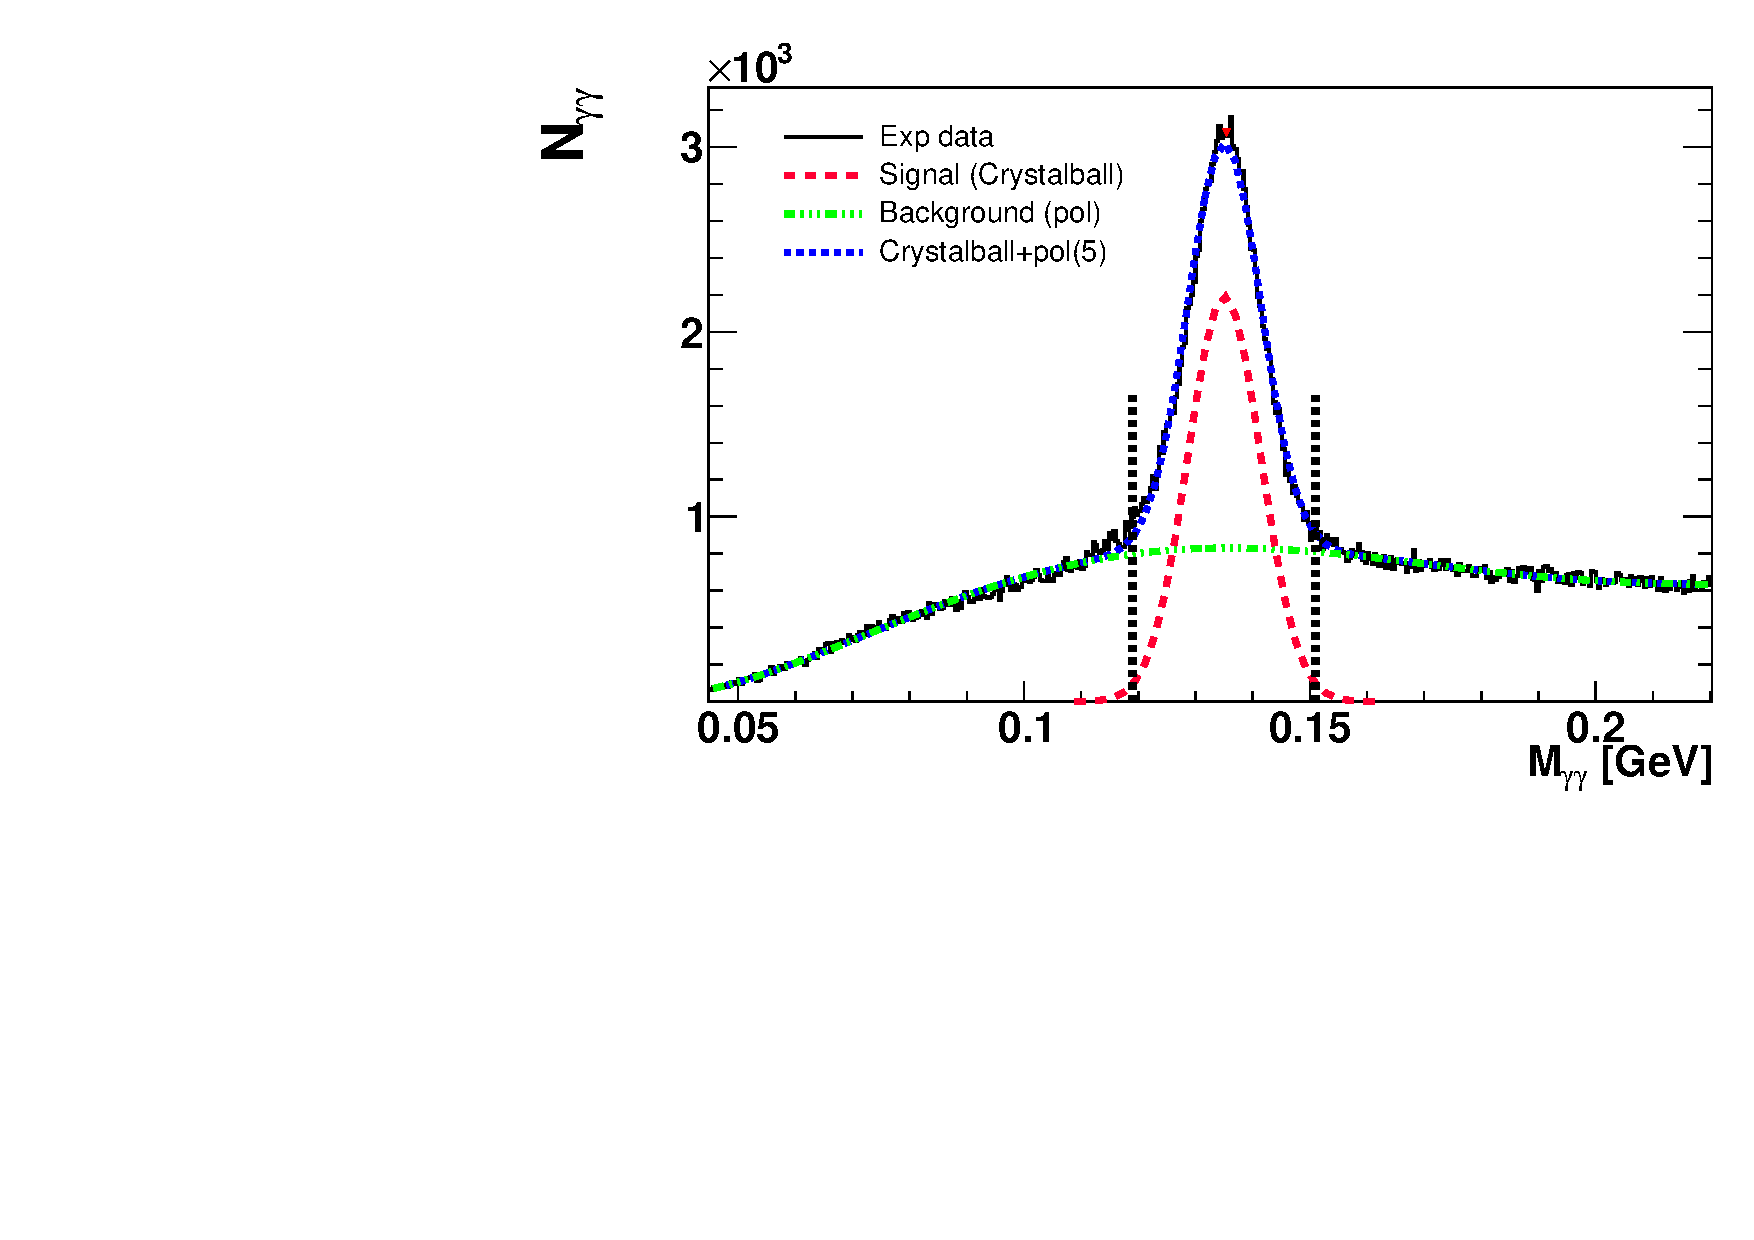
\includegraphics[width=.48\textwidth,natwidth=600,natheight=400]{figure_dataselection/pi0_crystalfit_Pt_0.pdf}}
  \subfigure[$P_t$ bin 1 (0.15 GeV $<P_t<$ 0.3 GeV)]{\label{fig:pi0fitpt1}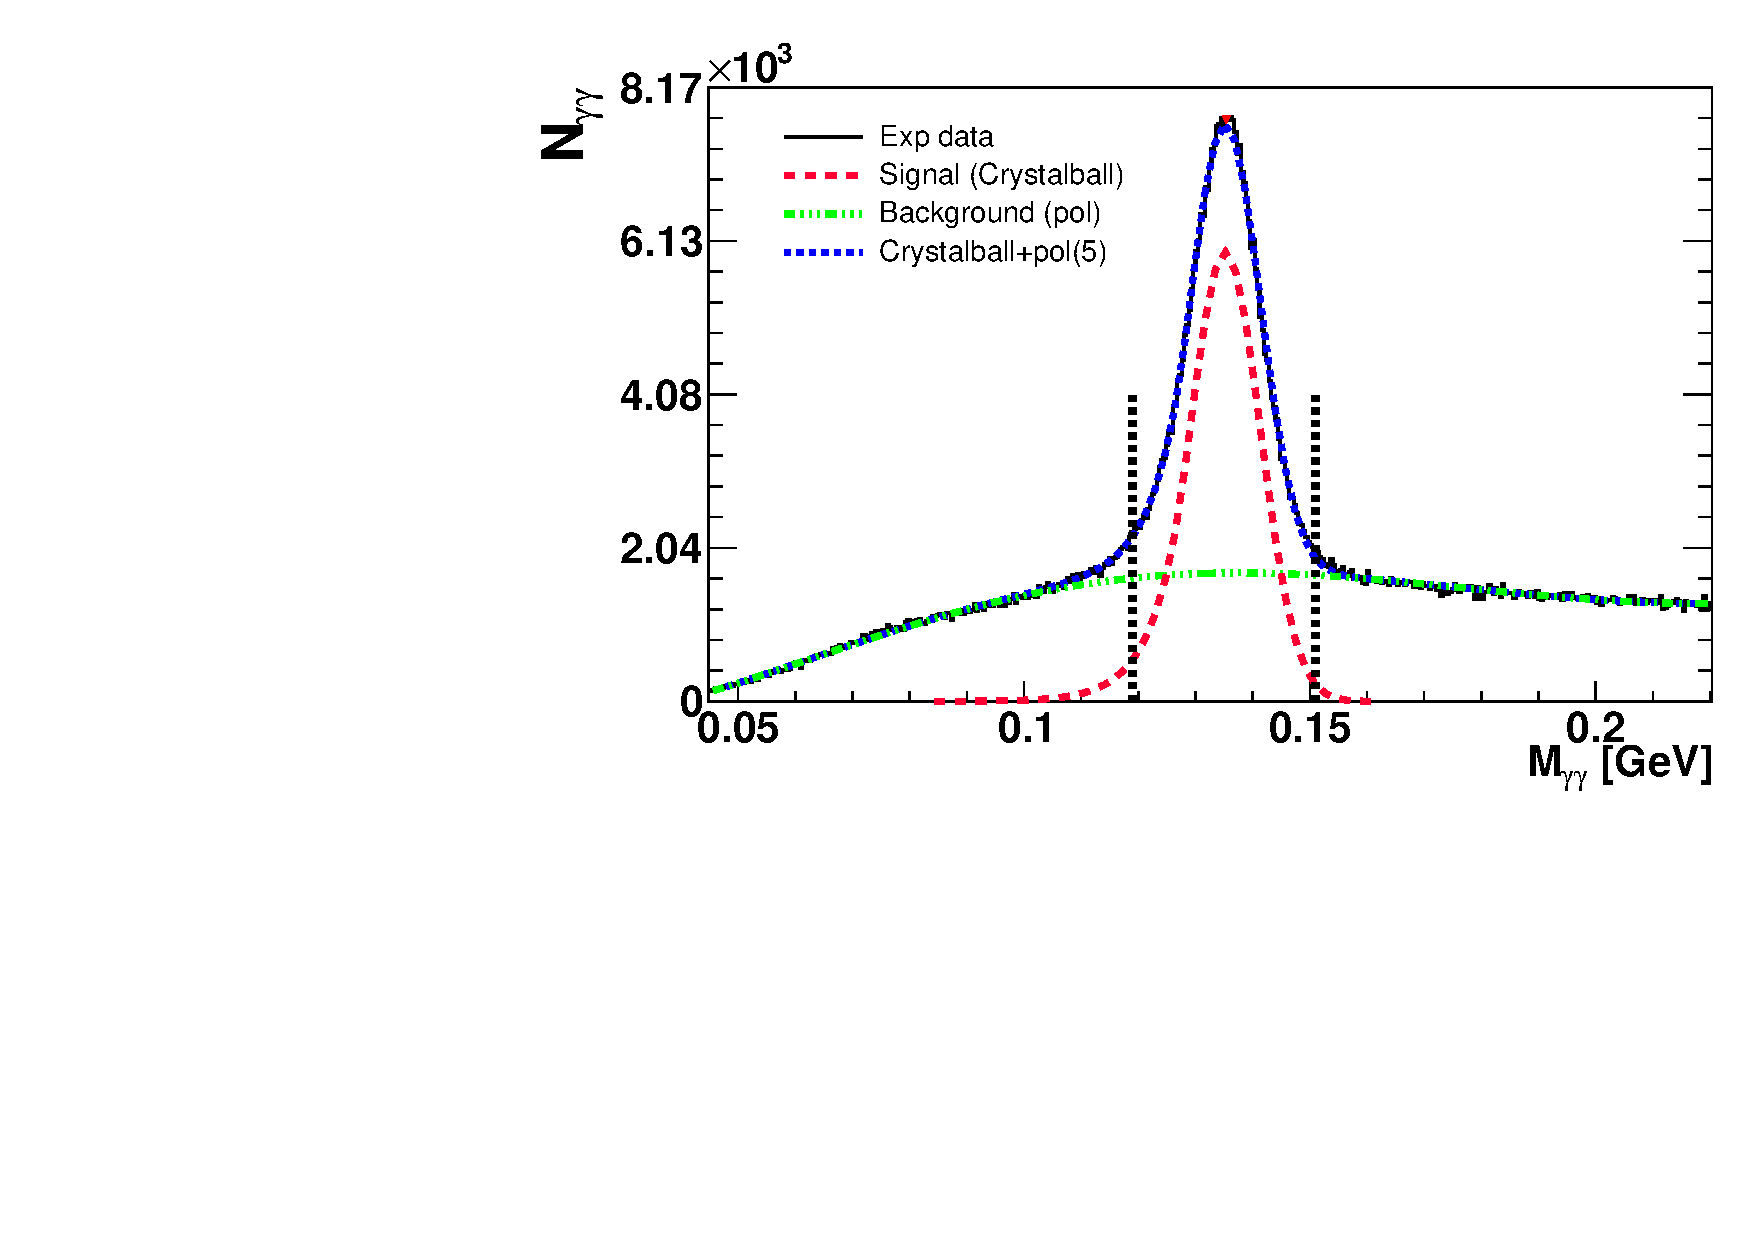
\includegraphics[width=.48\textwidth,natwidth=600,natheight=400]{figure_dataselection/pi0_crystalfit_Pt_1.pdf}}
  \subfigure[$P_t$ bin 2 (0.3 GeV $<P_t<$ 0.5 GeV)]{\label{fig:pi0fitpt2}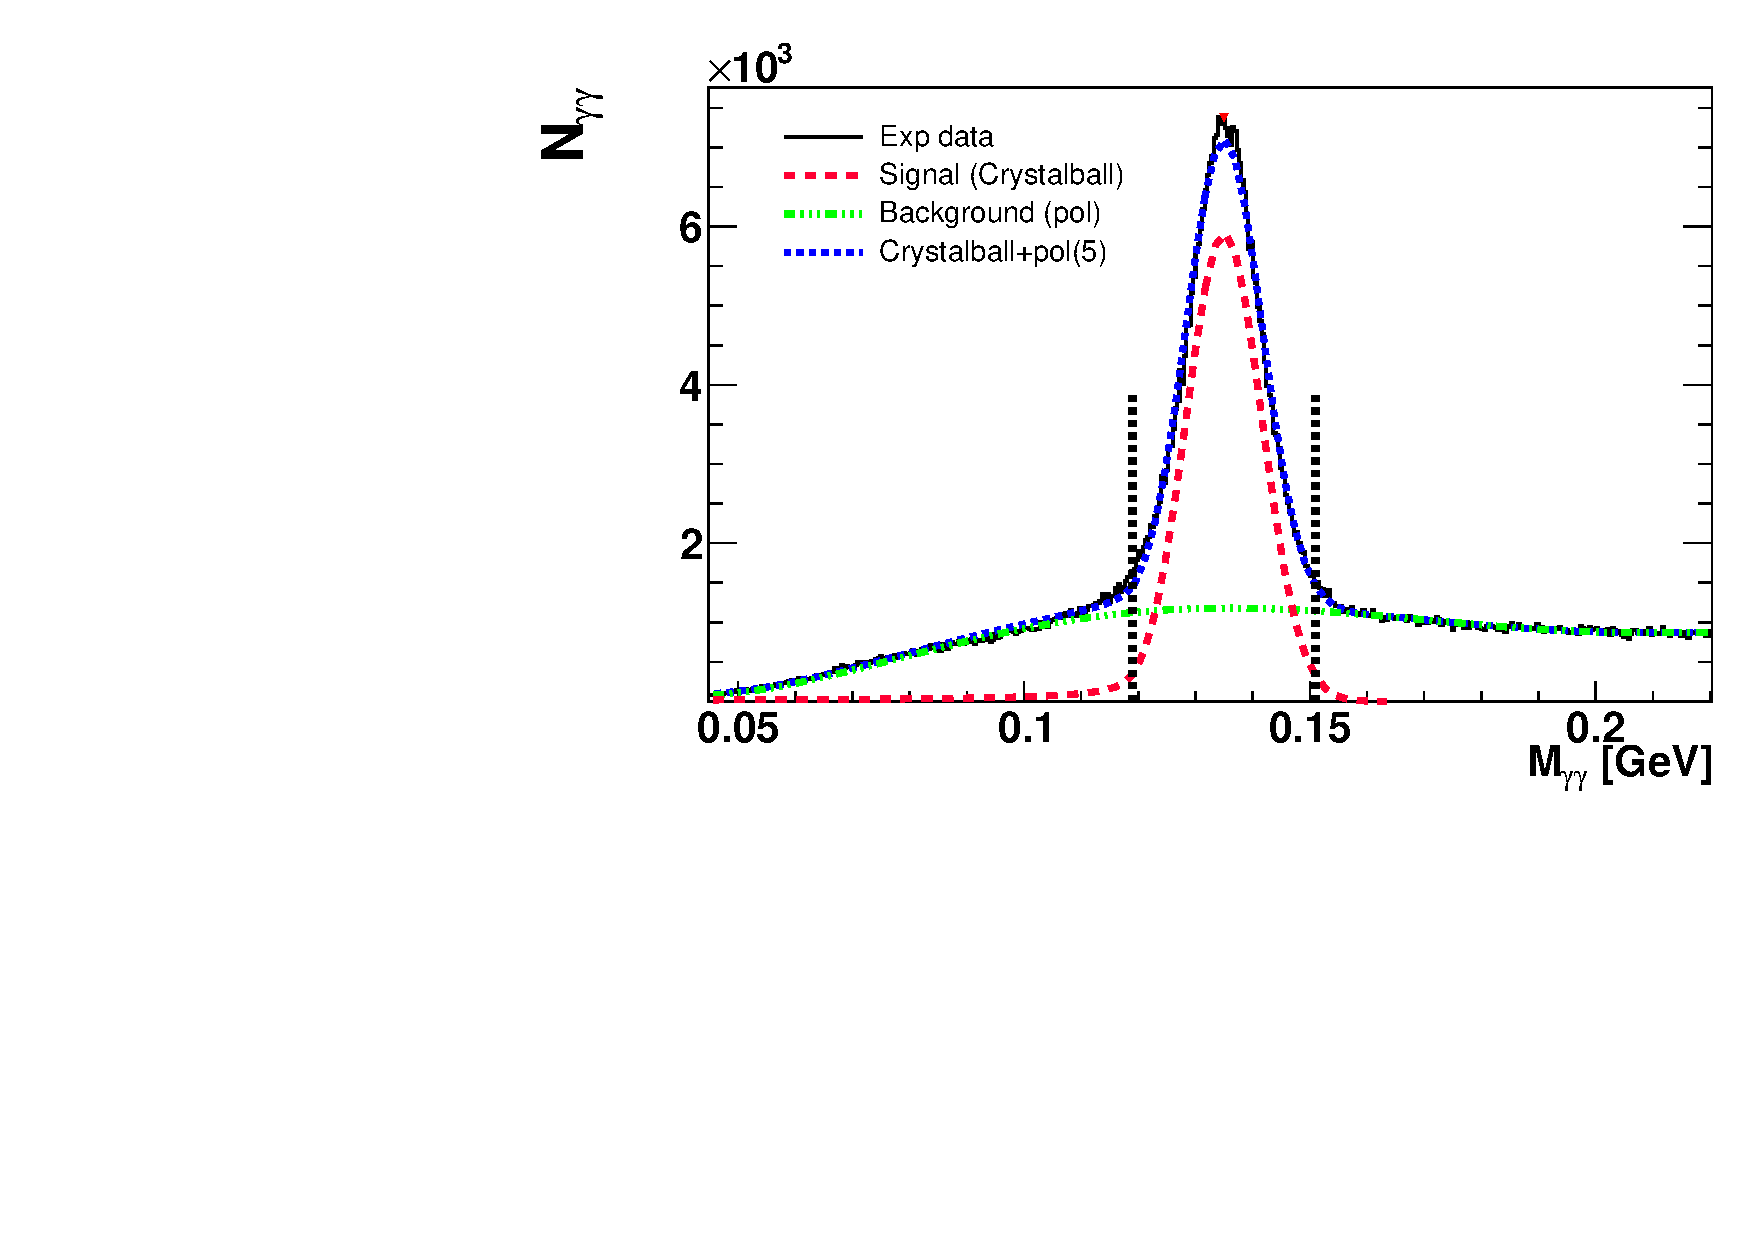
\includegraphics[width=.48\textwidth,natwidth=600,natheight=400]{figure_dataselection/pi0_crystalfit_Pt_2.pdf}}
  \subfigure[$P_t$ bin 3 (0.5 GeV $<P_t<$ 3 GeV)]{\label{fig:pi0fitpt3}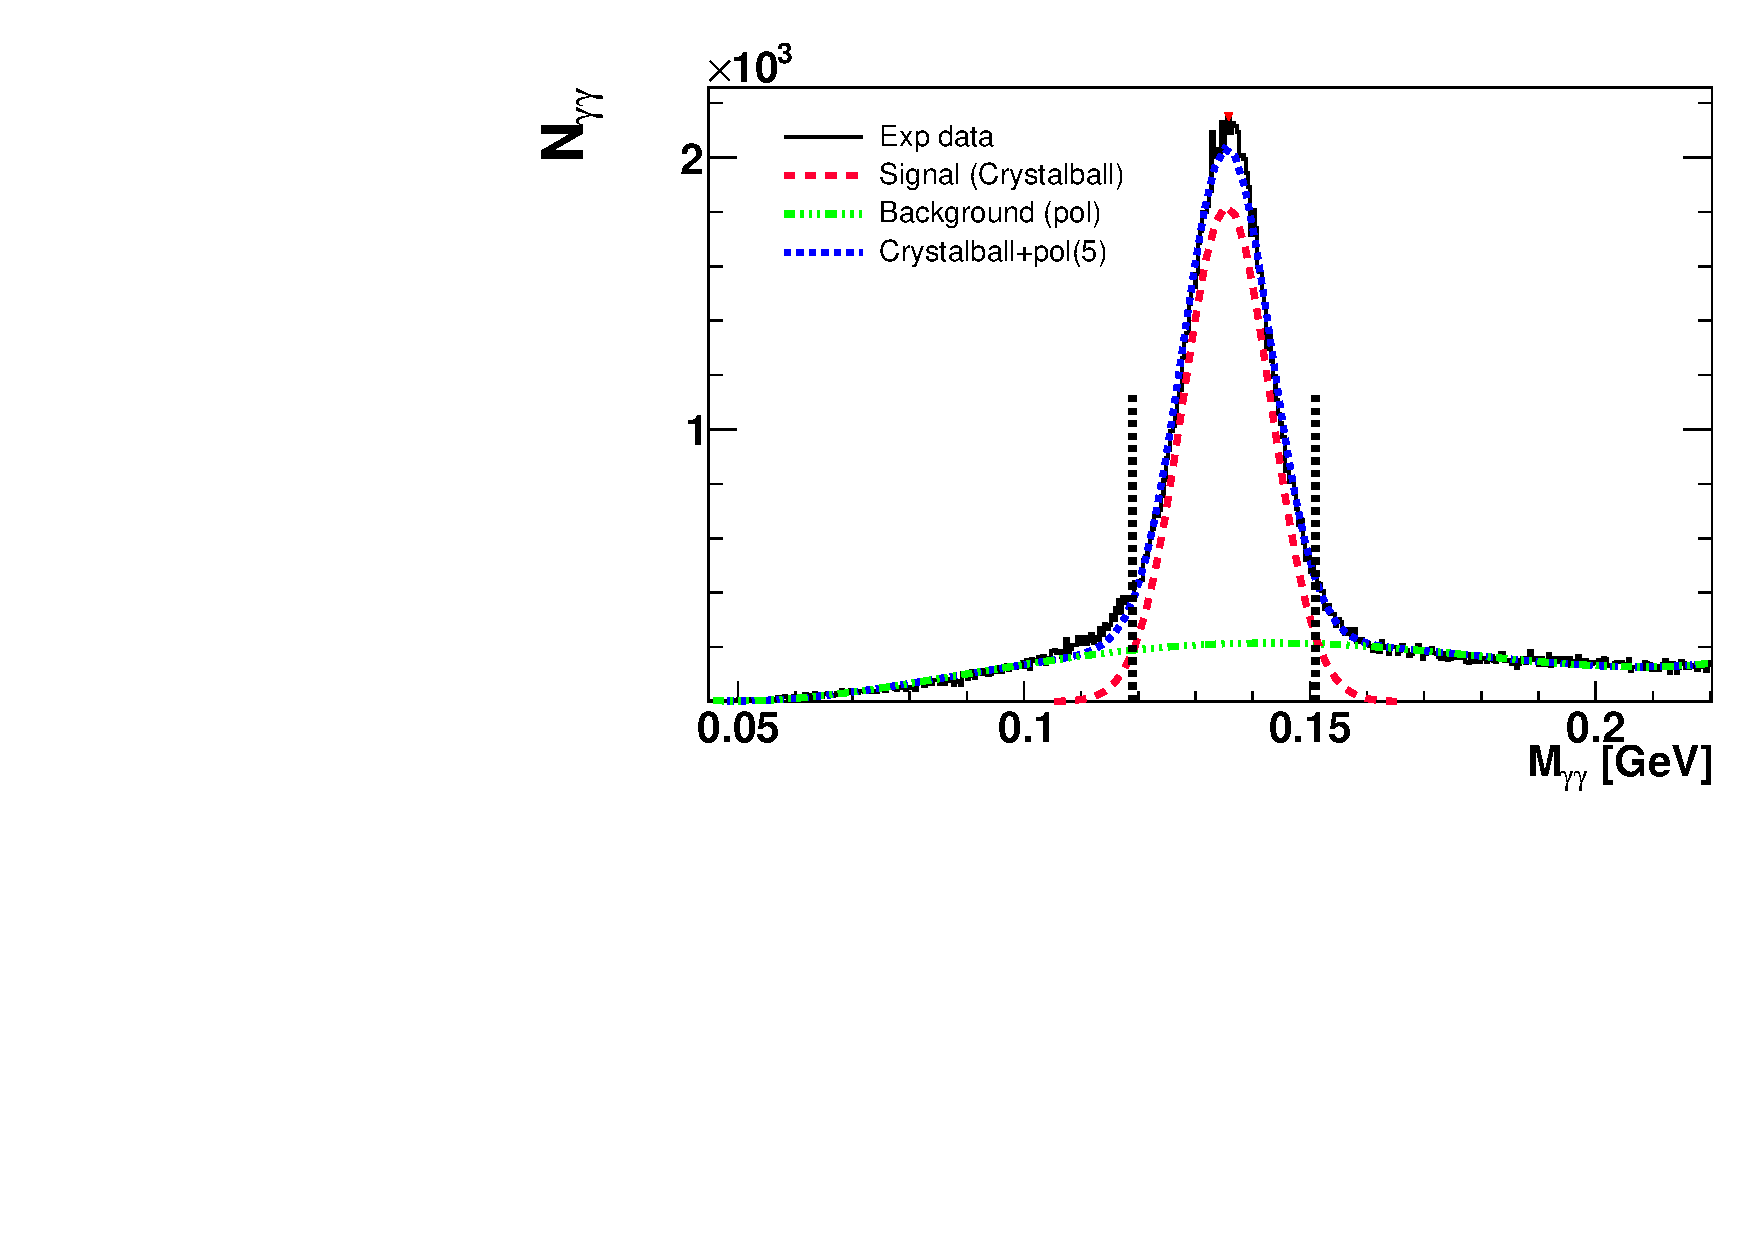
\includegraphics[width=.48\textwidth,natwidth=600,natheight=400]{figure_dataselection/pi0_crystalfit_Pt_3.pdf}}
  \caption[Crystal Ball fit for $\pi^0$ for all \(P_{t}\) bins]{Crystal Ball fit for $\pi^0$ for all \(P_{t}\) bins (default fit). Fit method as described in Section~\ref{sec:pi0fitsection}. Green dash-dotted line is the background and red dashed line is the signal.}
  \label{fig:pi0ptfit}
\end{figure}

\begin{figure}[H]
  \centering     \tiny
  \subfigure[$z$ bin 0 ($0.1<z<0.2$)]{\label{fig:pi0fitz1}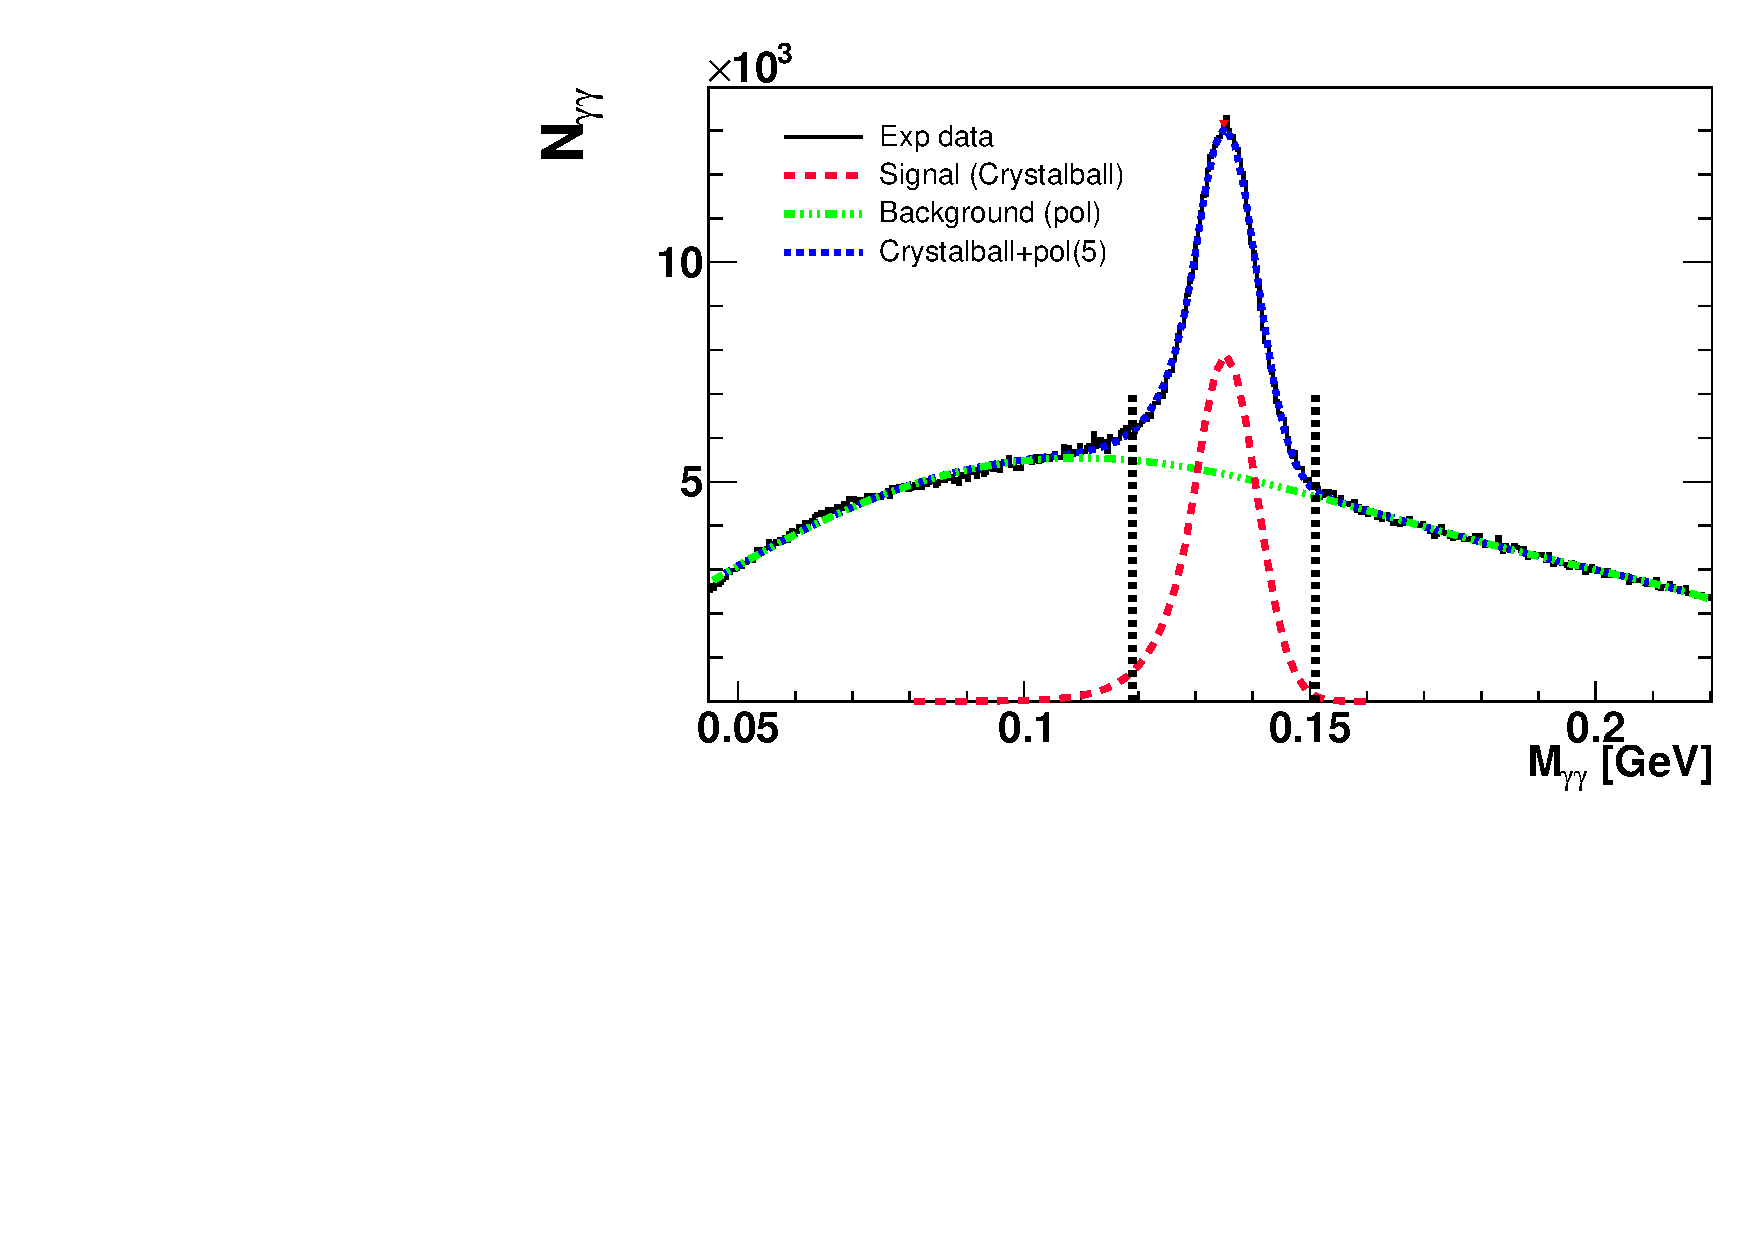
\includegraphics[width=.48\textwidth,natwidth=600,natheight=400]{figure_dataselection/pi0_crystalfit_Z_0.pdf}}
  \subfigure[$z$ bin 1 ($0.2<z<0.3$)]{\label{fig:pi0fitz2}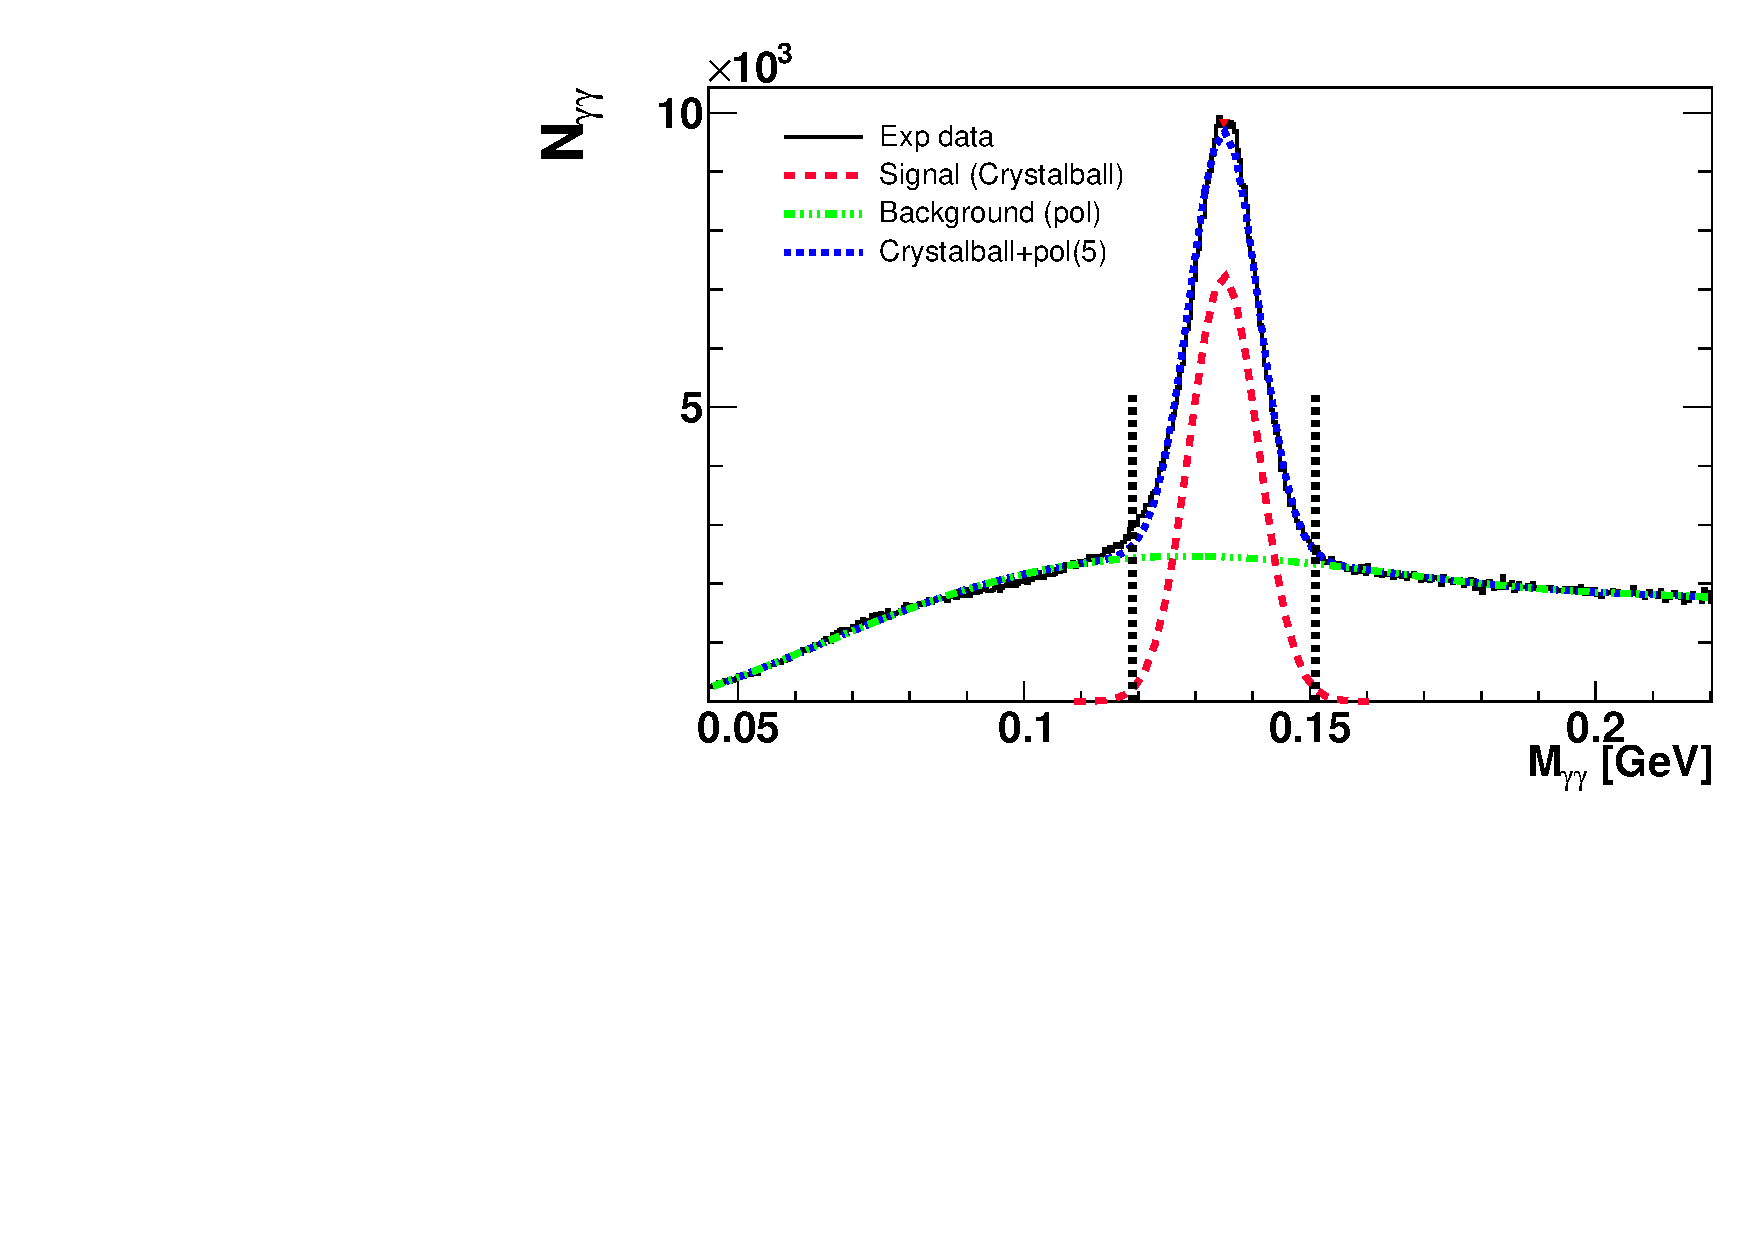
\includegraphics[width=.48\textwidth,natwidth=600,natheight=400]{figure_dataselection/pi0_crystalfit_Z_1.pdf}}
  \subfigure[$z$ bin 2 ($0.3<z<0.4$)]{\label{fig:pi0fitz3}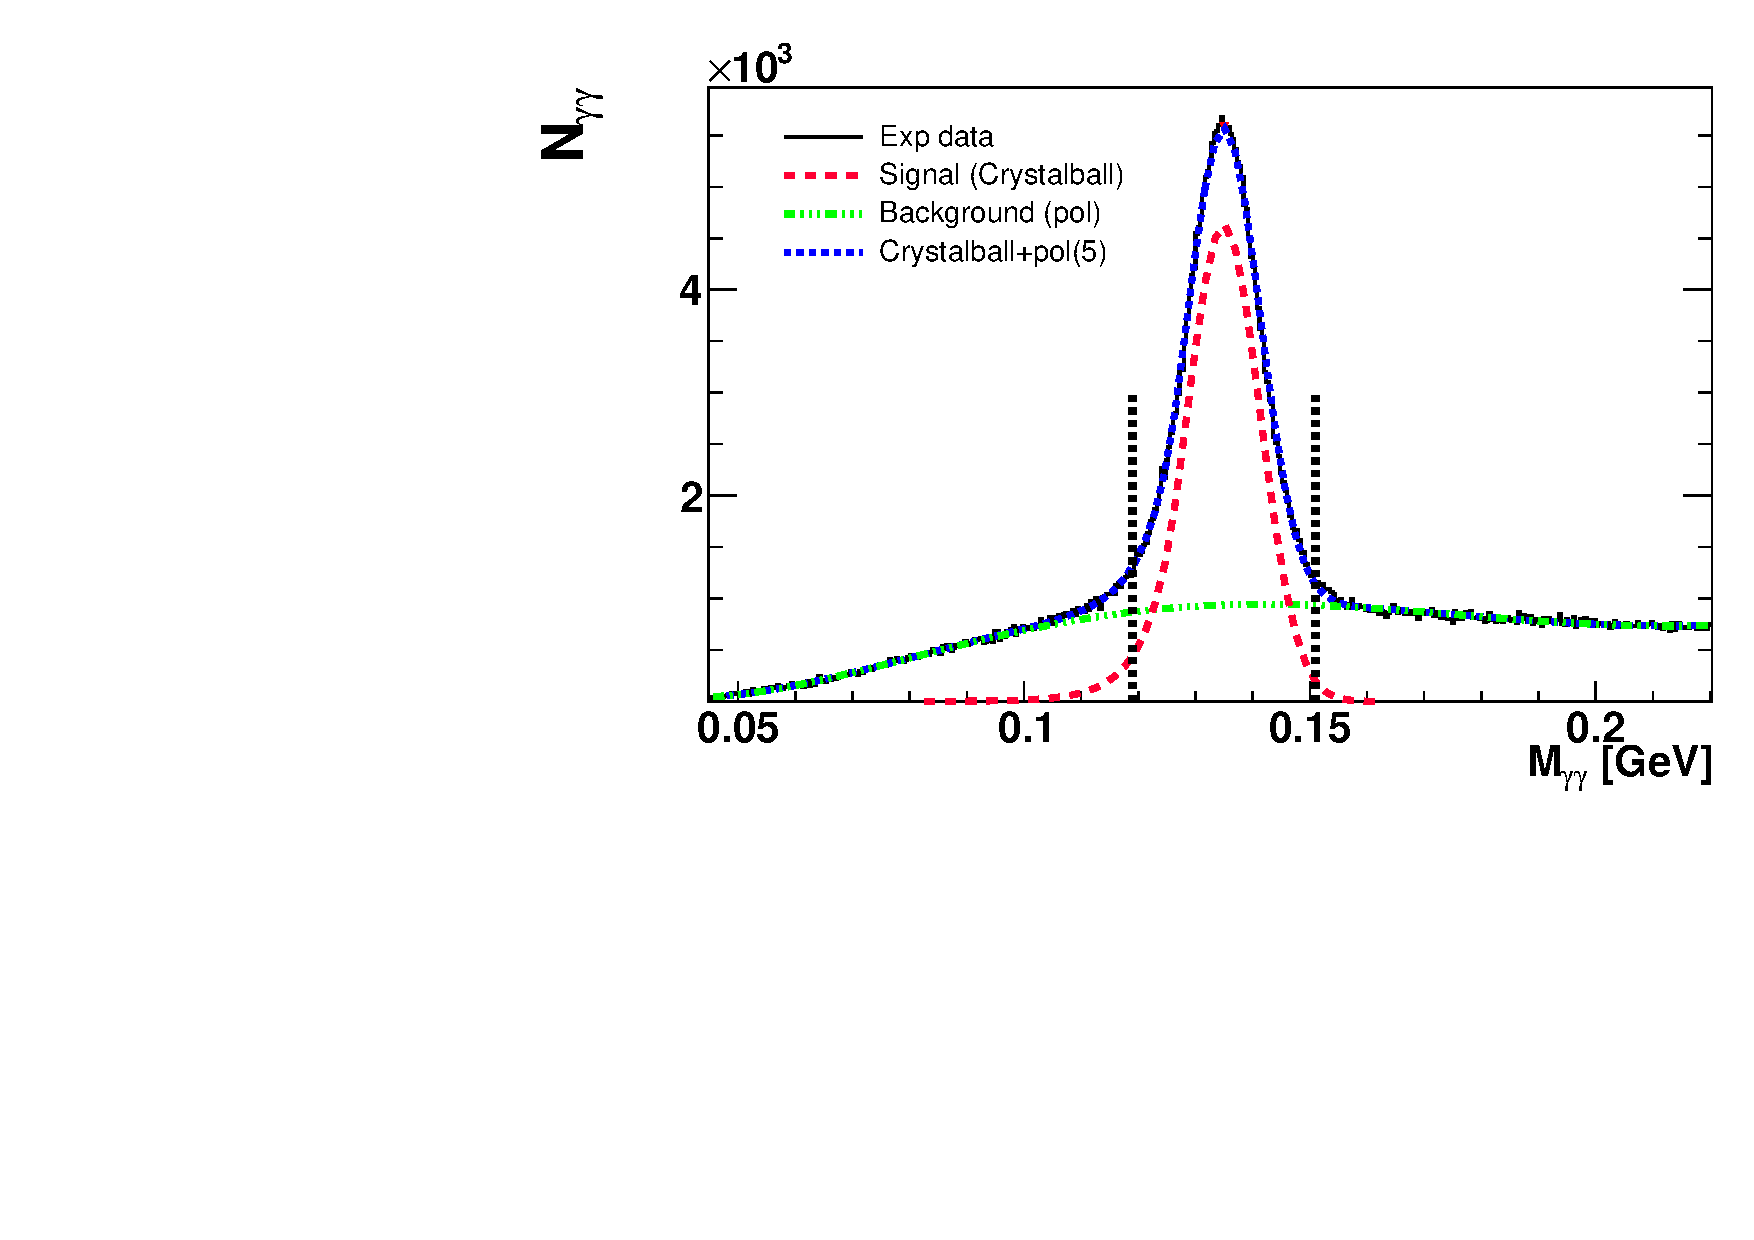
\includegraphics[width=.48\textwidth,natwidth=600,natheight=400]{figure_dataselection/pi0_crystalfit_Z_2.pdf}}
  \subfigure[$z$ bin 3 ($0.4<z<0.5$)]{\label{fig:pi0fitz4}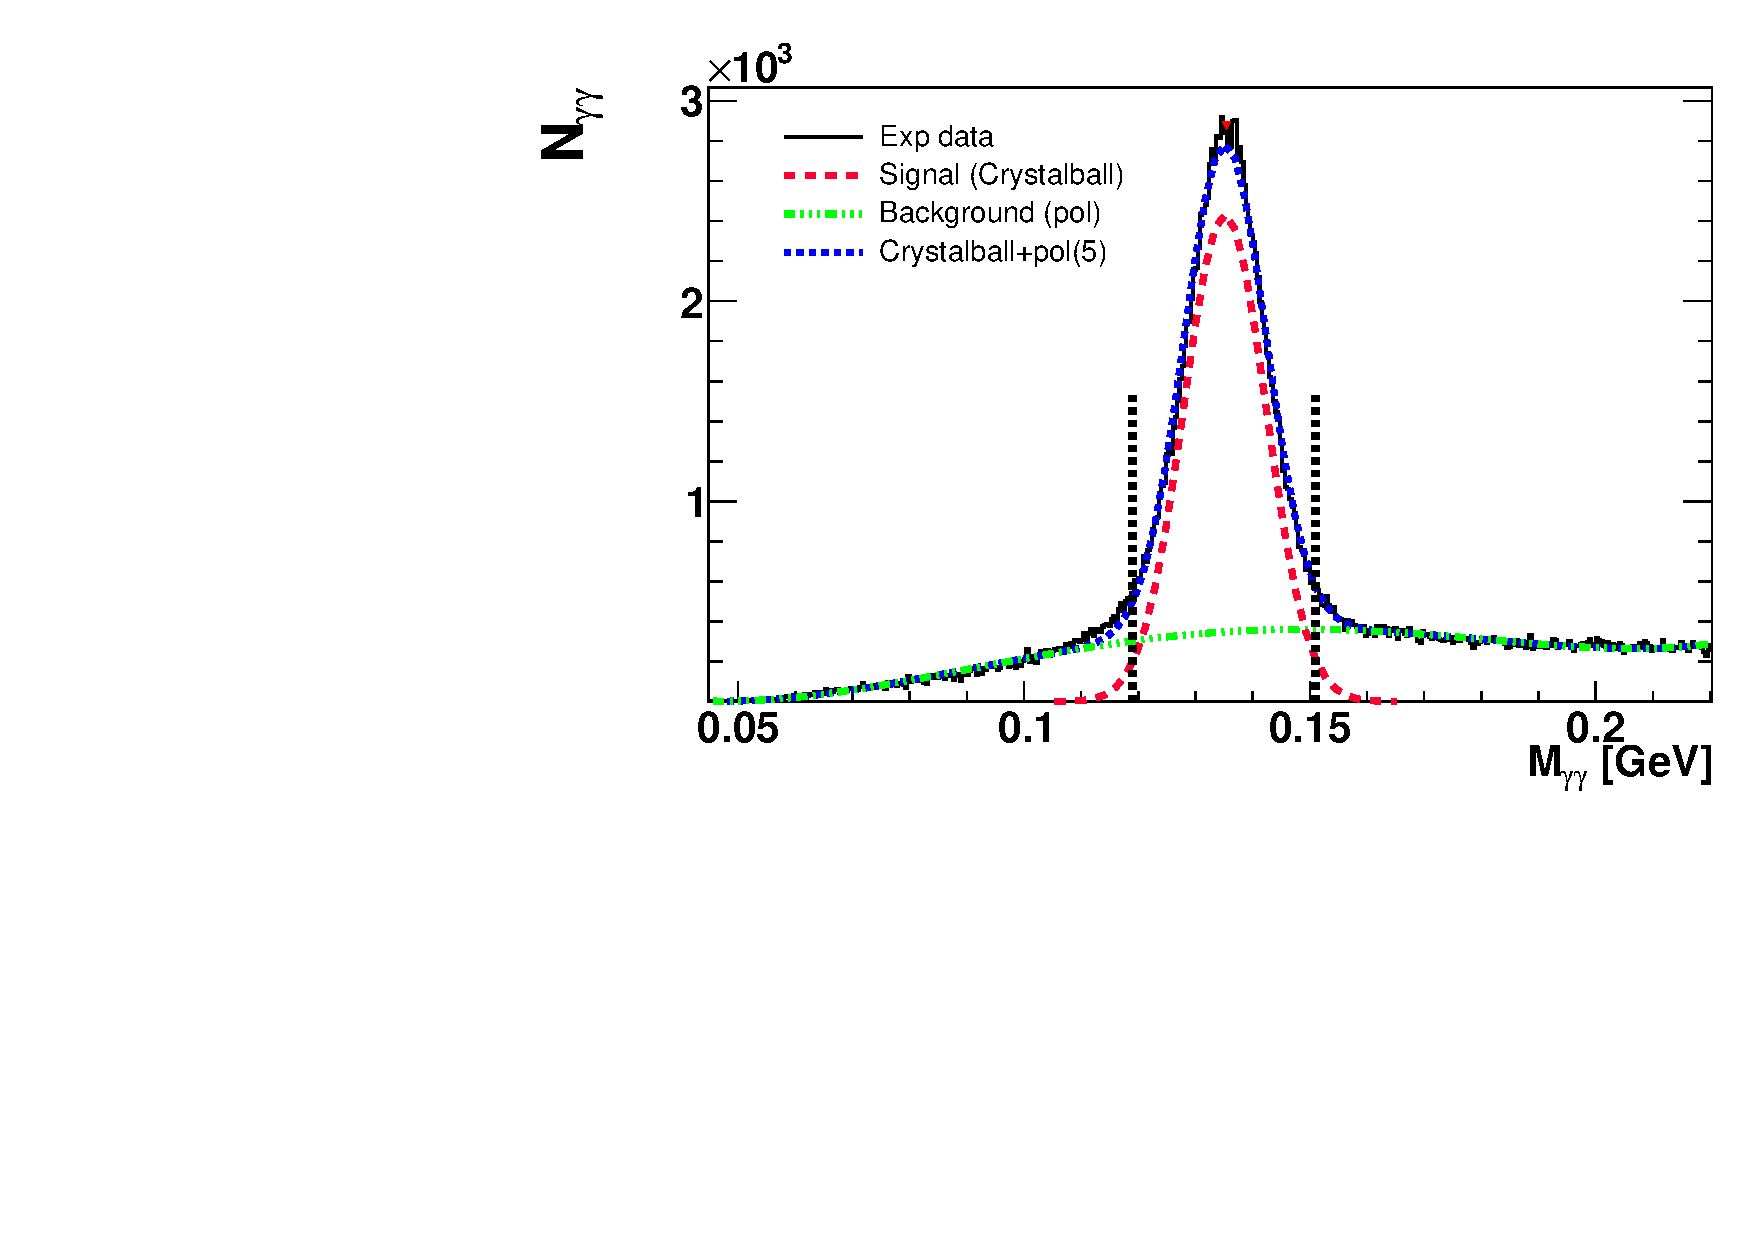
\includegraphics[width=.48\textwidth,natwidth=600,natheight=400]{figure_dataselection/pi0_crystalfit_Z_3.pdf}}
  \subfigure[$z$ bin 4 ($0.5<z<0.6$)]{\label{fig:pi0fitz5}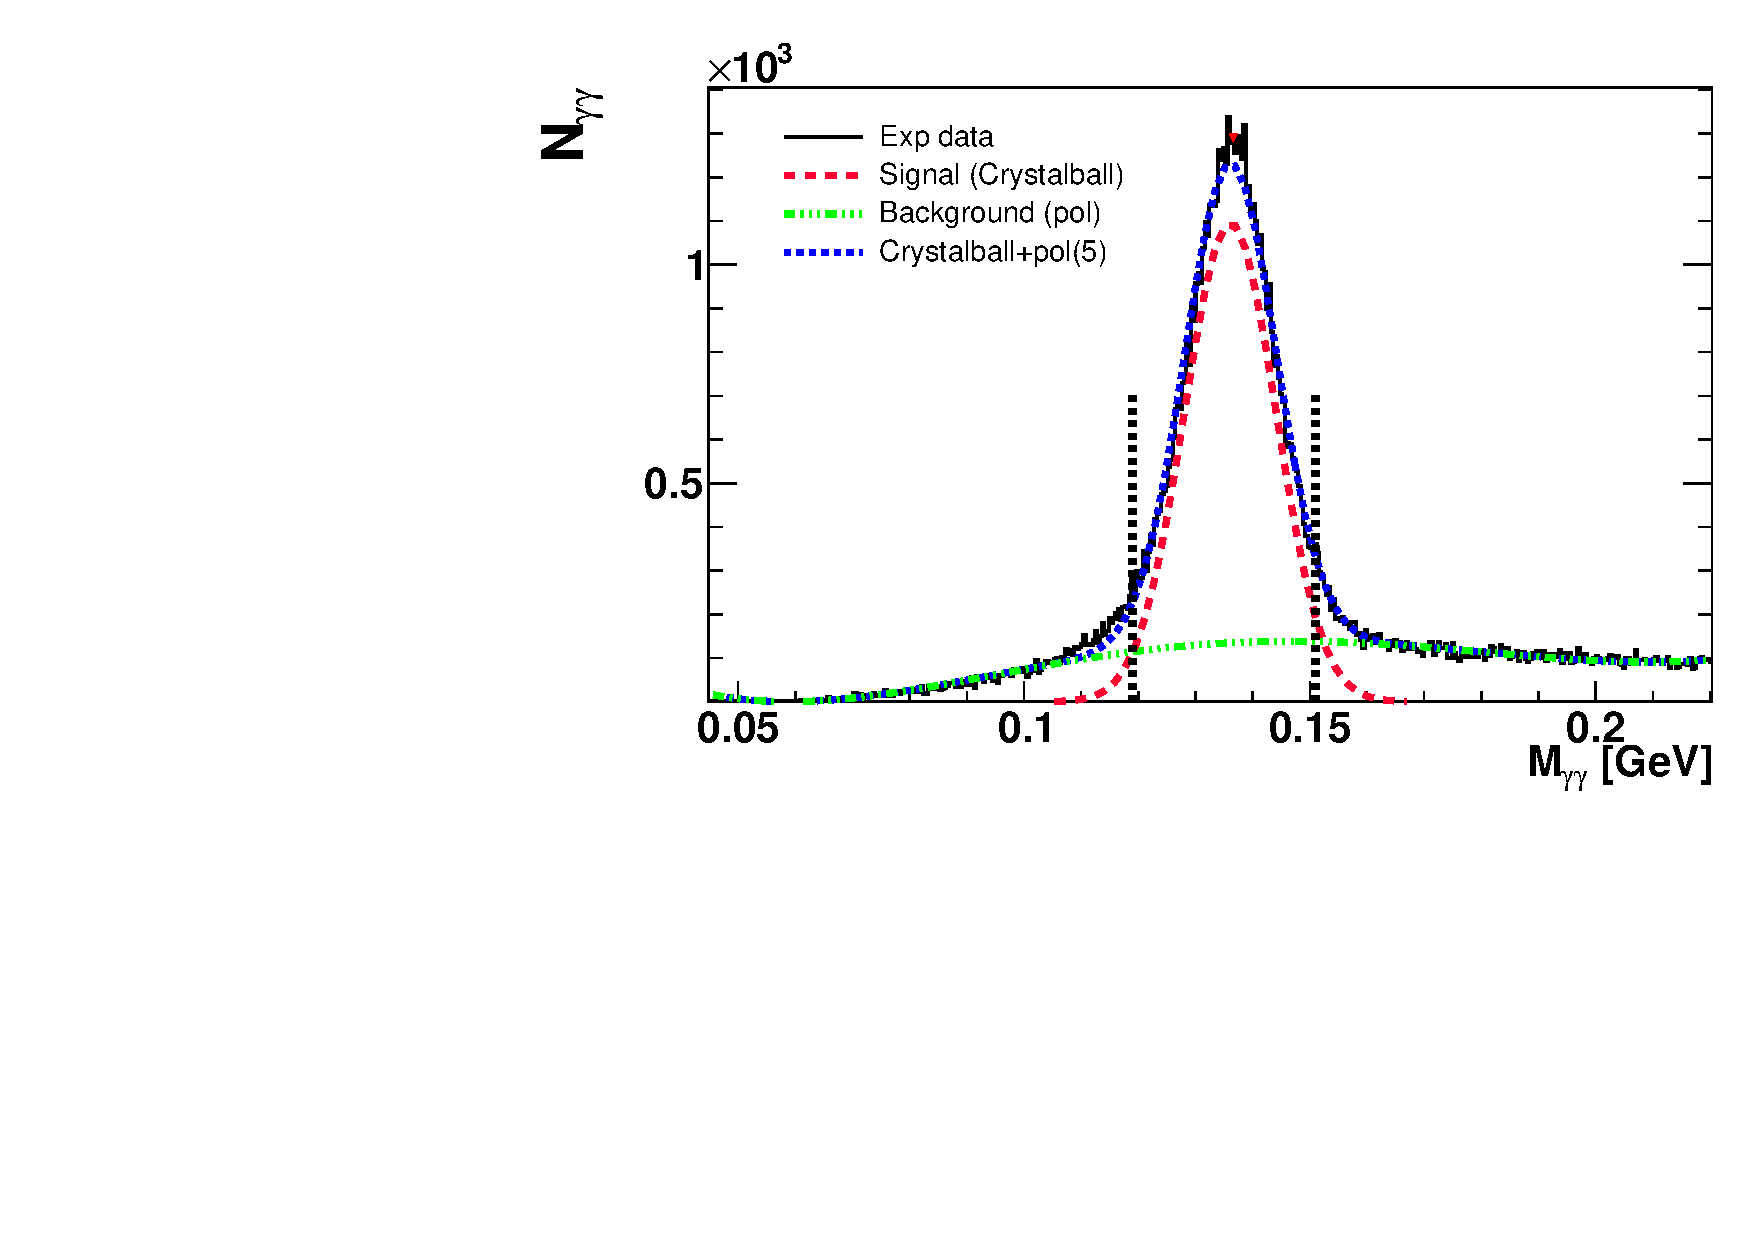
\includegraphics[width=.48\textwidth,natwidth=600,natheight=400]{figure_dataselection/pi0_crystalfit_Z_4.pdf}}
  \subfigure[$z$ bin 5 ($0.6<z<0.7$)]{\label{fig:pi0fitz6}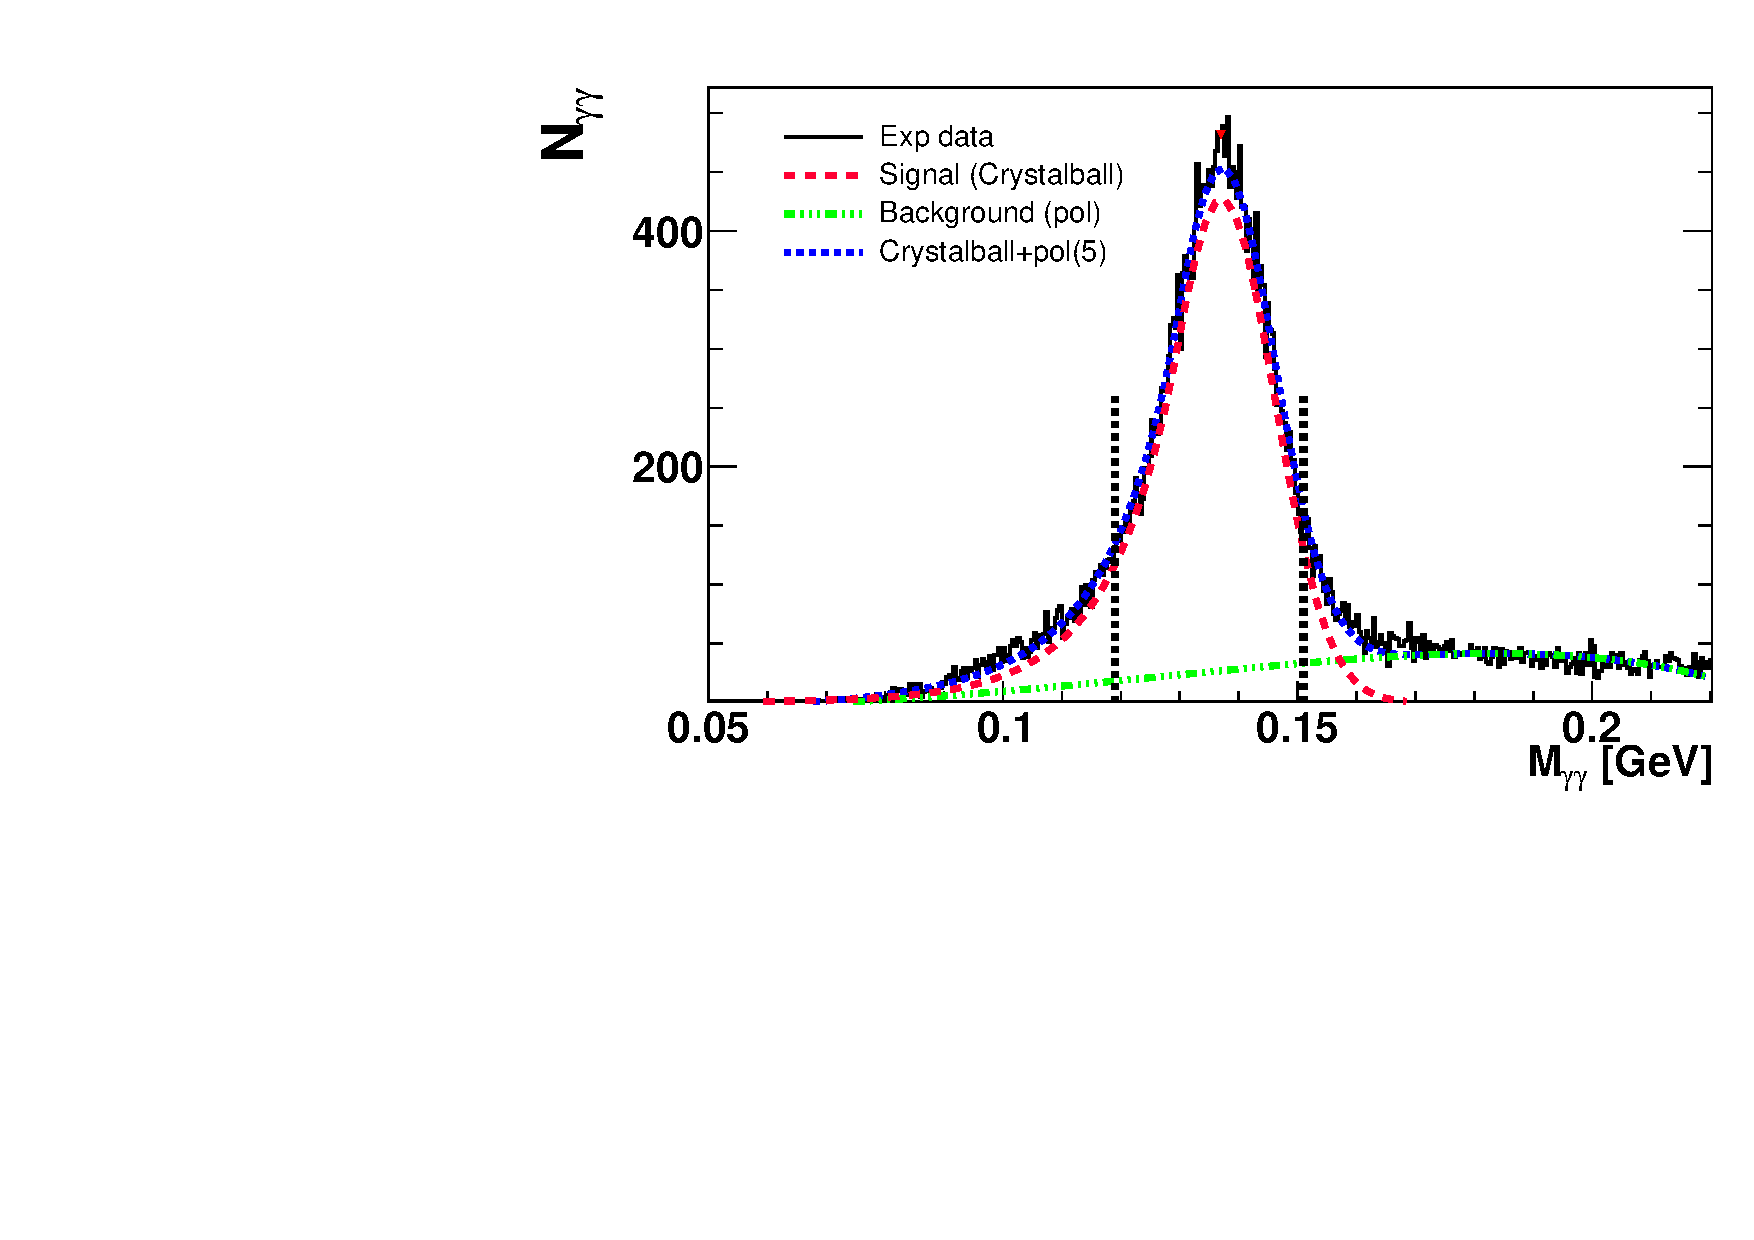
\includegraphics[width=.48\textwidth,natwidth=600,natheight=400]{figure_dataselection/pi0_crystalfit_Z_5.pdf}}
  \subfigure[$z$ bin 6 ($0.7<z<1$)]{\label{fig:pi0fitz7}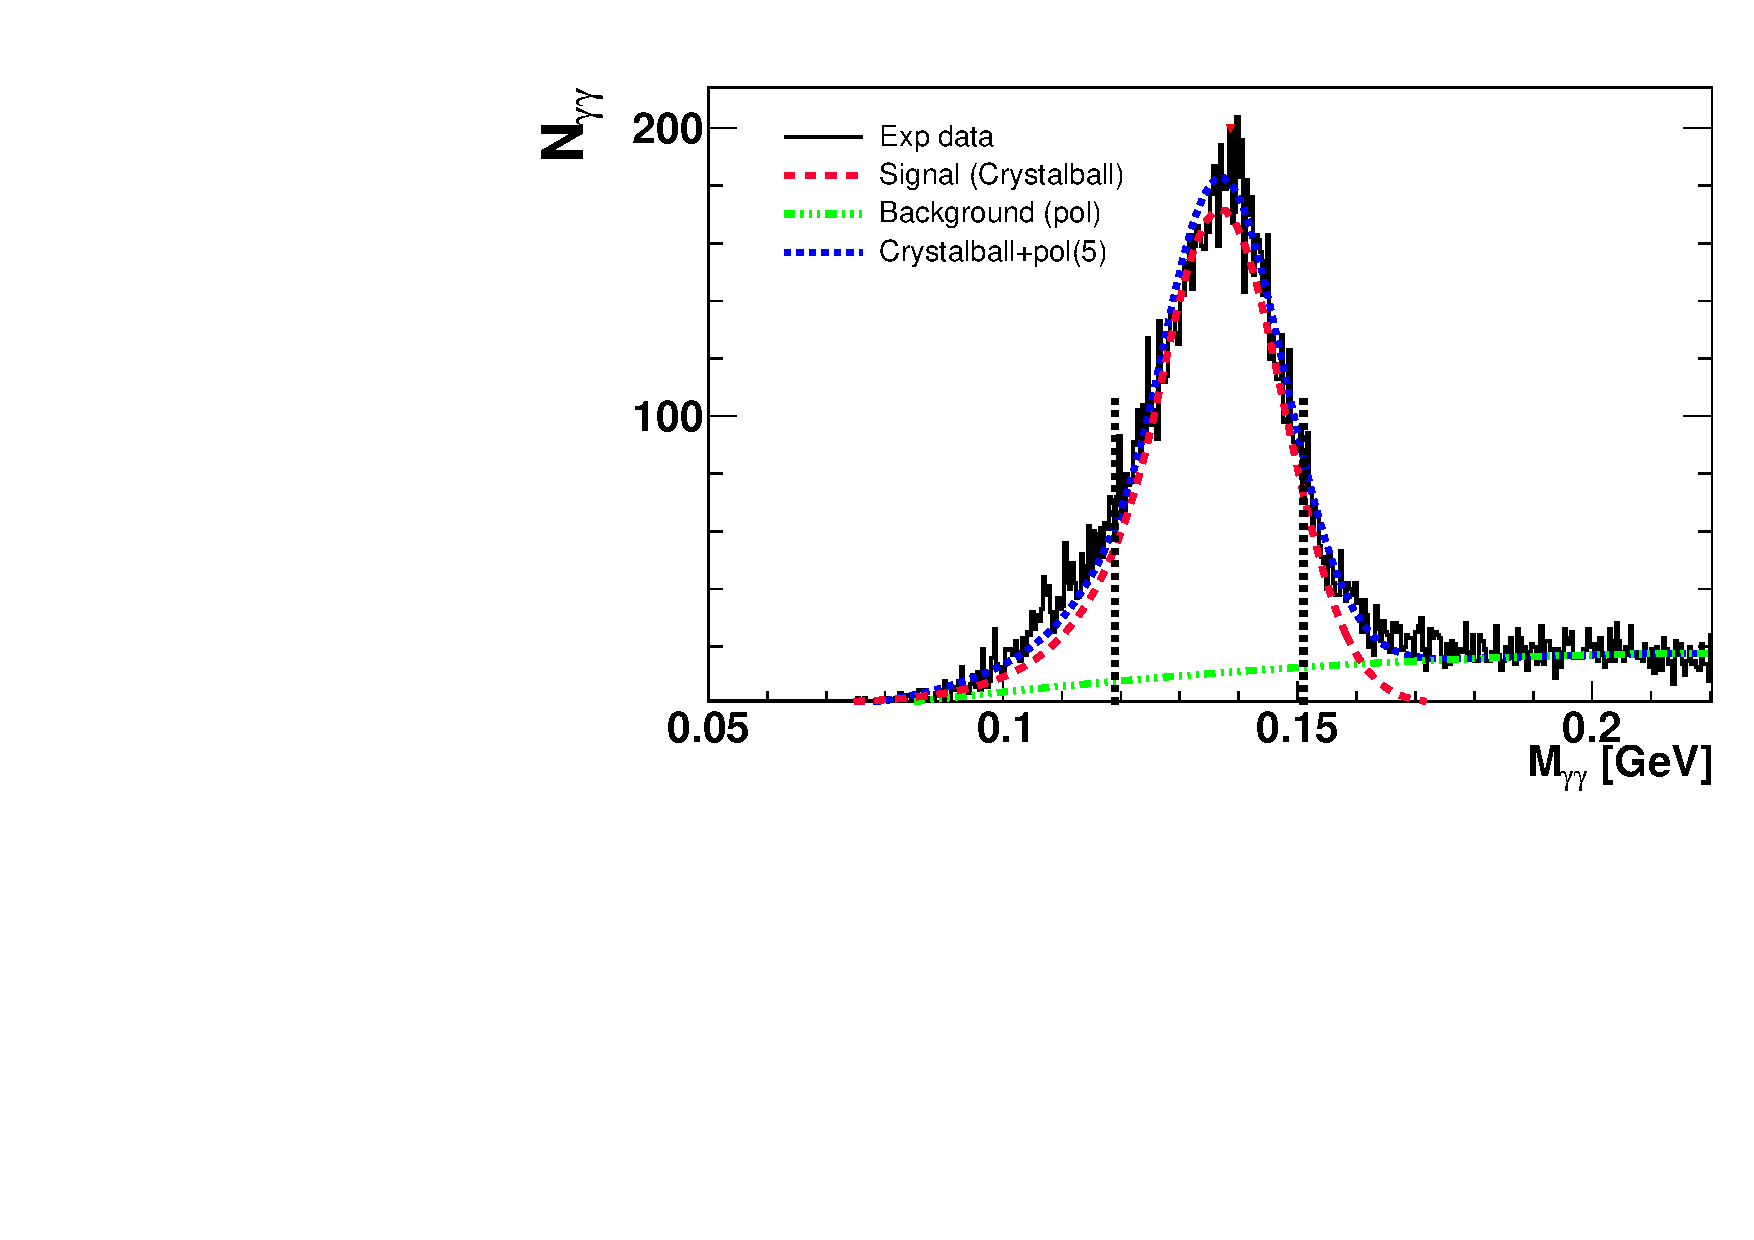
\includegraphics[width=.48\textwidth,natwidth=600,natheight=400]{figure_dataselection/pi0_crystalfit_Z_6.pdf}}
\label{fig:pi0zfit}
\caption[Crystal Ball fit for $\pi^0$ for all \(z\) bins]{Crystal Ball fit for $\pi^0$ for all \(z\) bins (default fit). Fit method as described in Section~\ref{sec:pi0fitsection}. Green dash-dotted line is the background and red dashed line is the signal.}
\end{figure}



\subsubsection{\texorpdfstring{Fit with MC Background of $\pi^0$ for all kinematic bins}{Fit with MC Background of pi0 for all kinematic bins}}
\label{sec:bkgfitpi0}

\begin{figure}[H]
  \centering
  \subfigure[$P_t$ bin 0 ($P_t<$ 0.15 GeV)]{\label{fig:pi0fitpt0}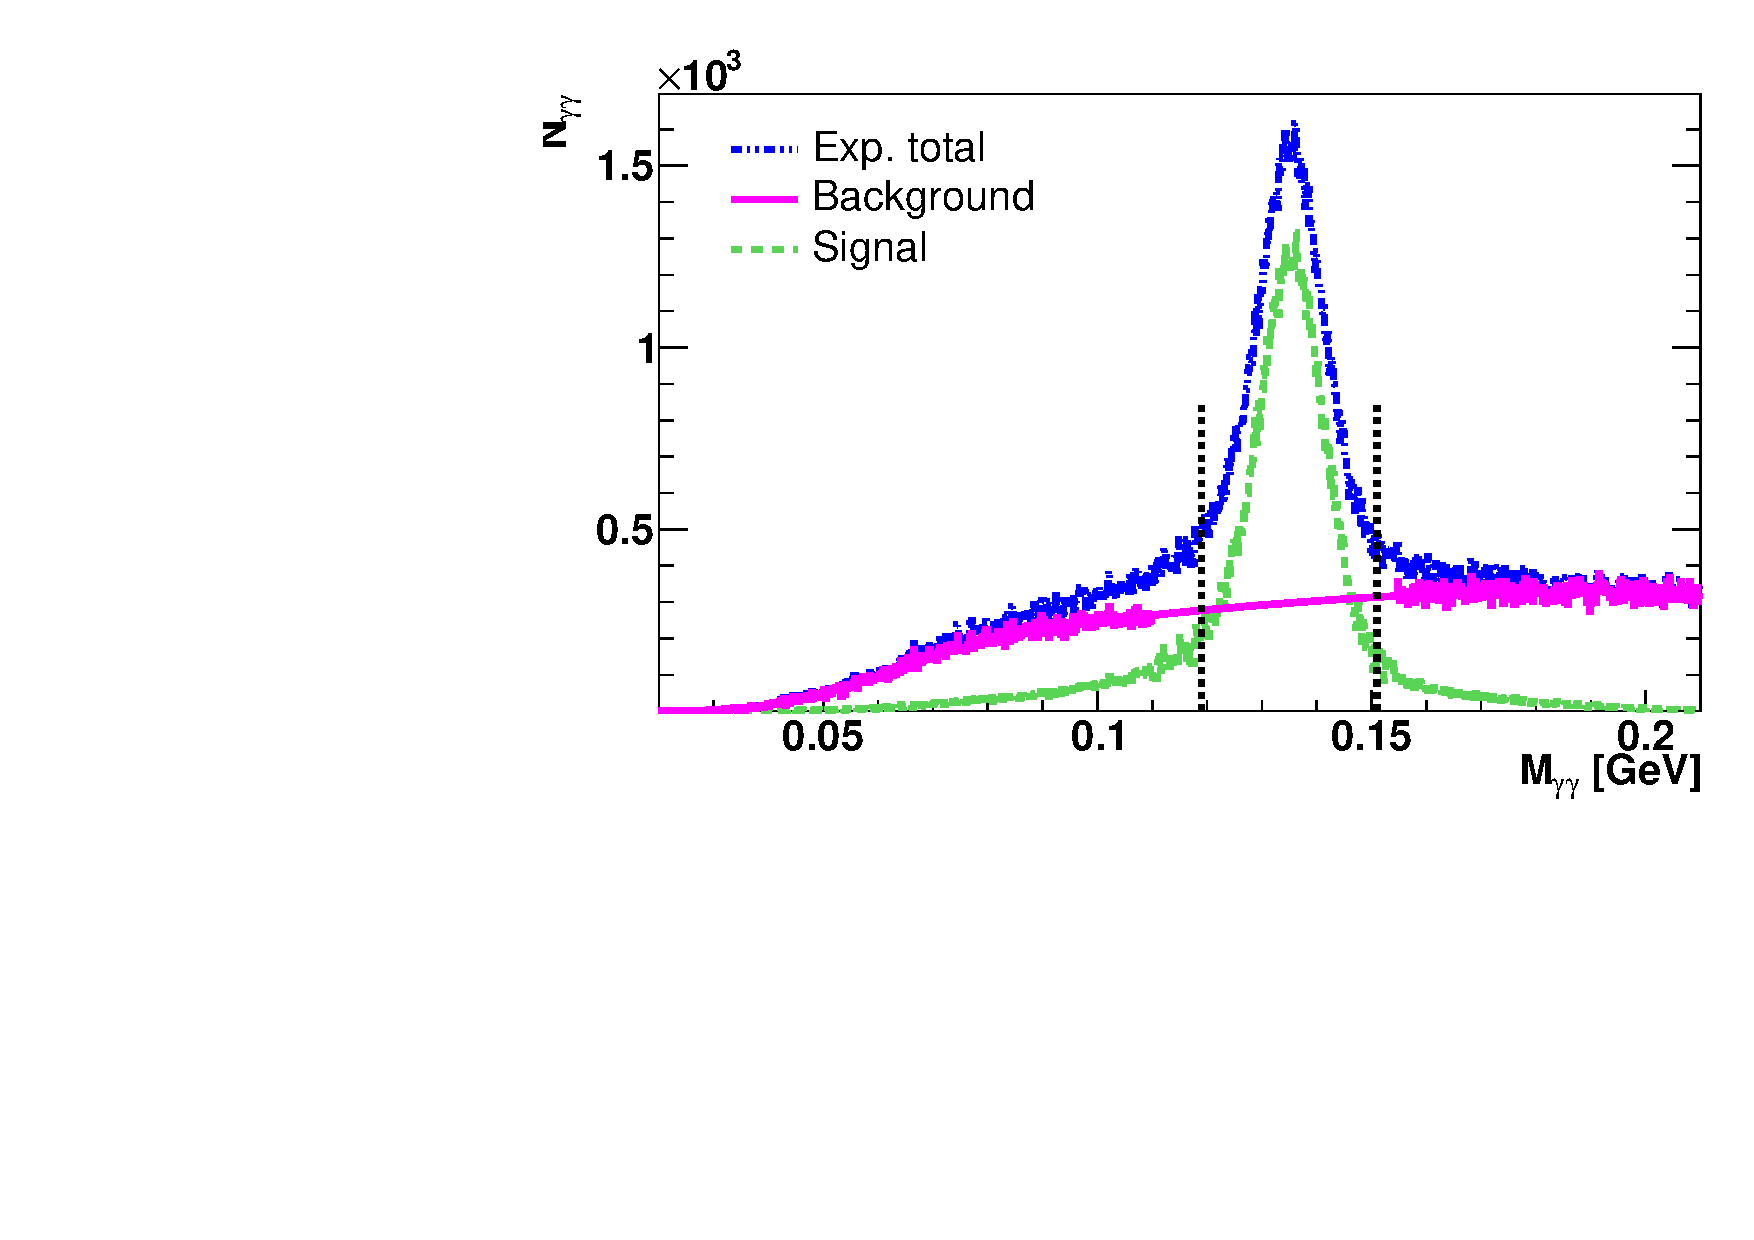
\includegraphics[width=.48\textwidth,natwidth=600,natheight=400]{figure_dataselection/pi0_fit_Pt_0.pdf}}
  \subfigure[$P_t$ bin 1 (0.15 GeV $<P_t<$ 0.3 GeV)]{\label{fig:pi0fitpt1}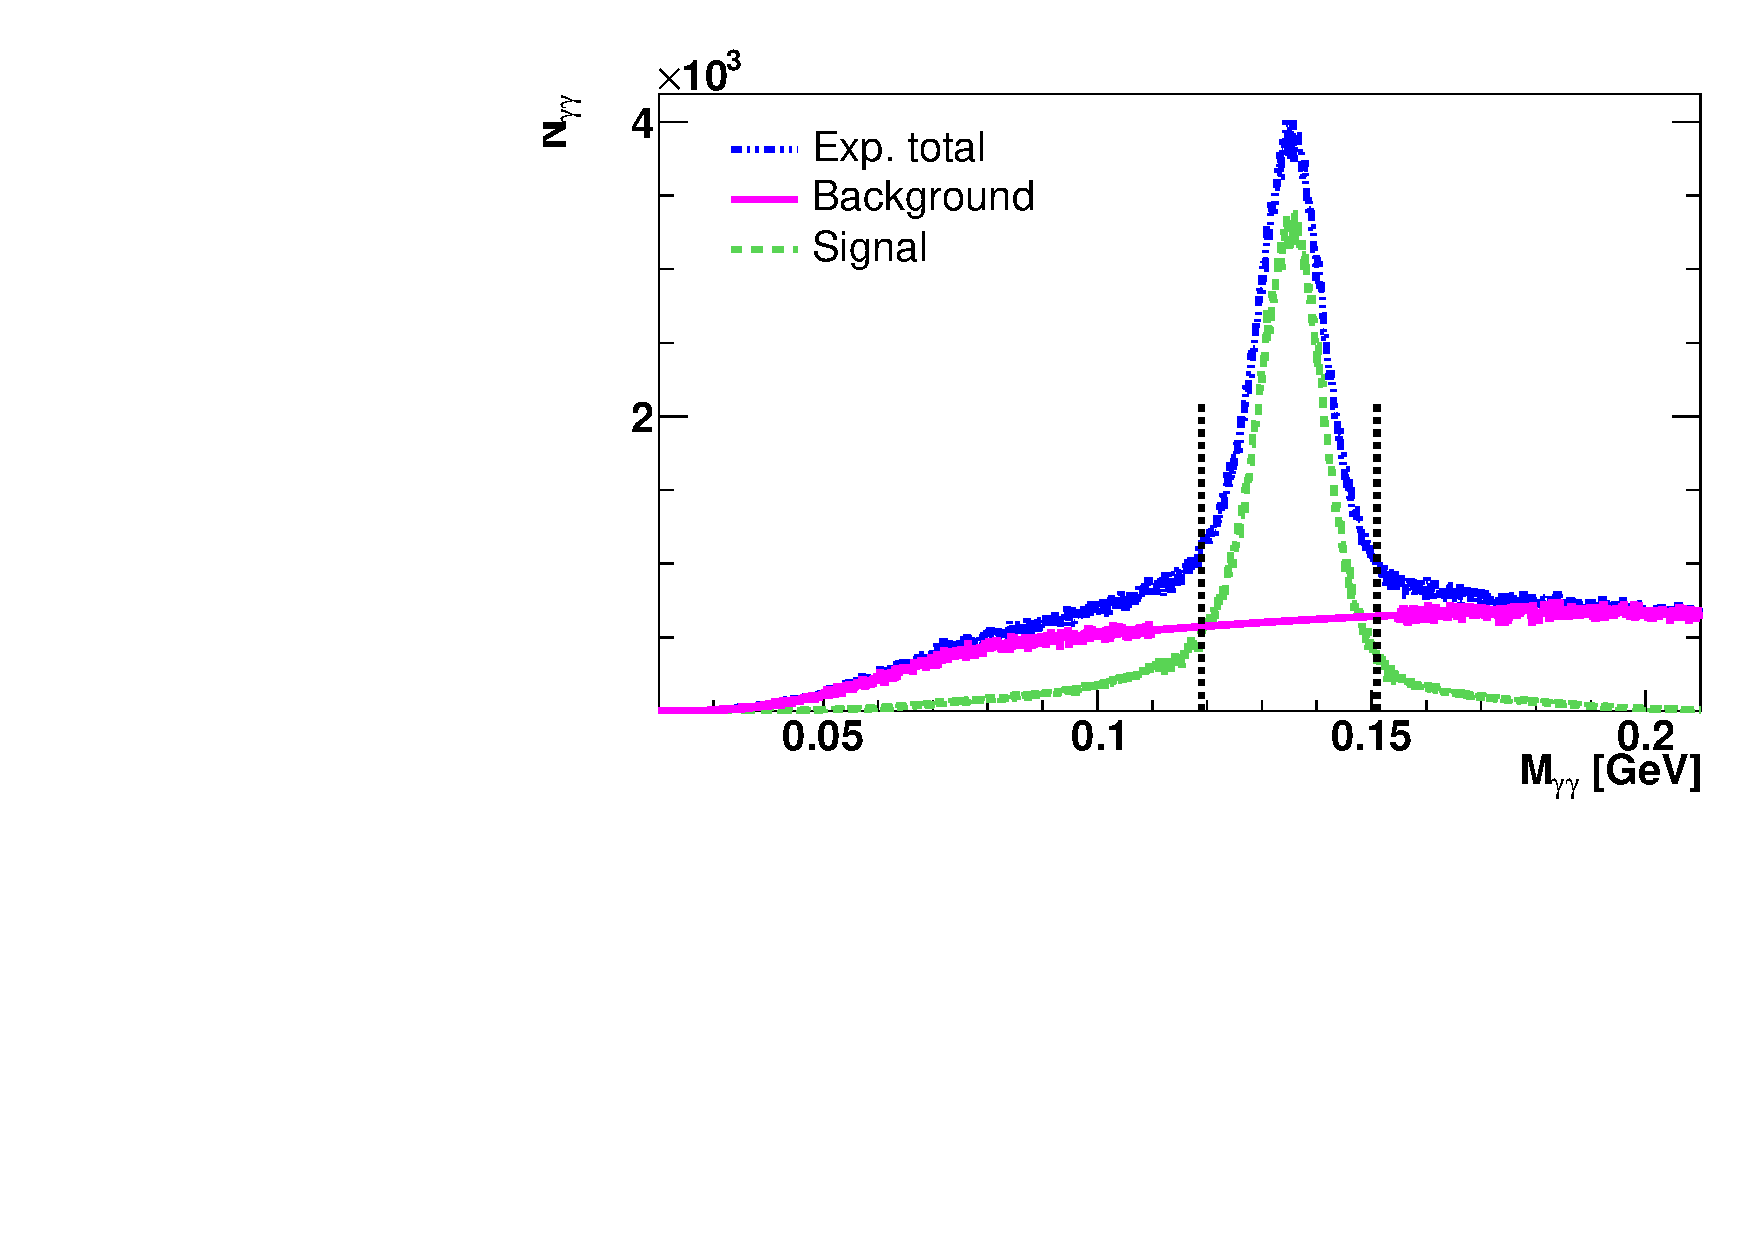
\includegraphics[width=.48\textwidth,natwidth=600,natheight=400]{figure_dataselection/pi0_fit_Pt_1.pdf}}
  \subfigure[$P_t$ bin 2 (0.3 GeV $<P_t<$ 0.5 GeV)]{\label{fig:pi0fitpt2}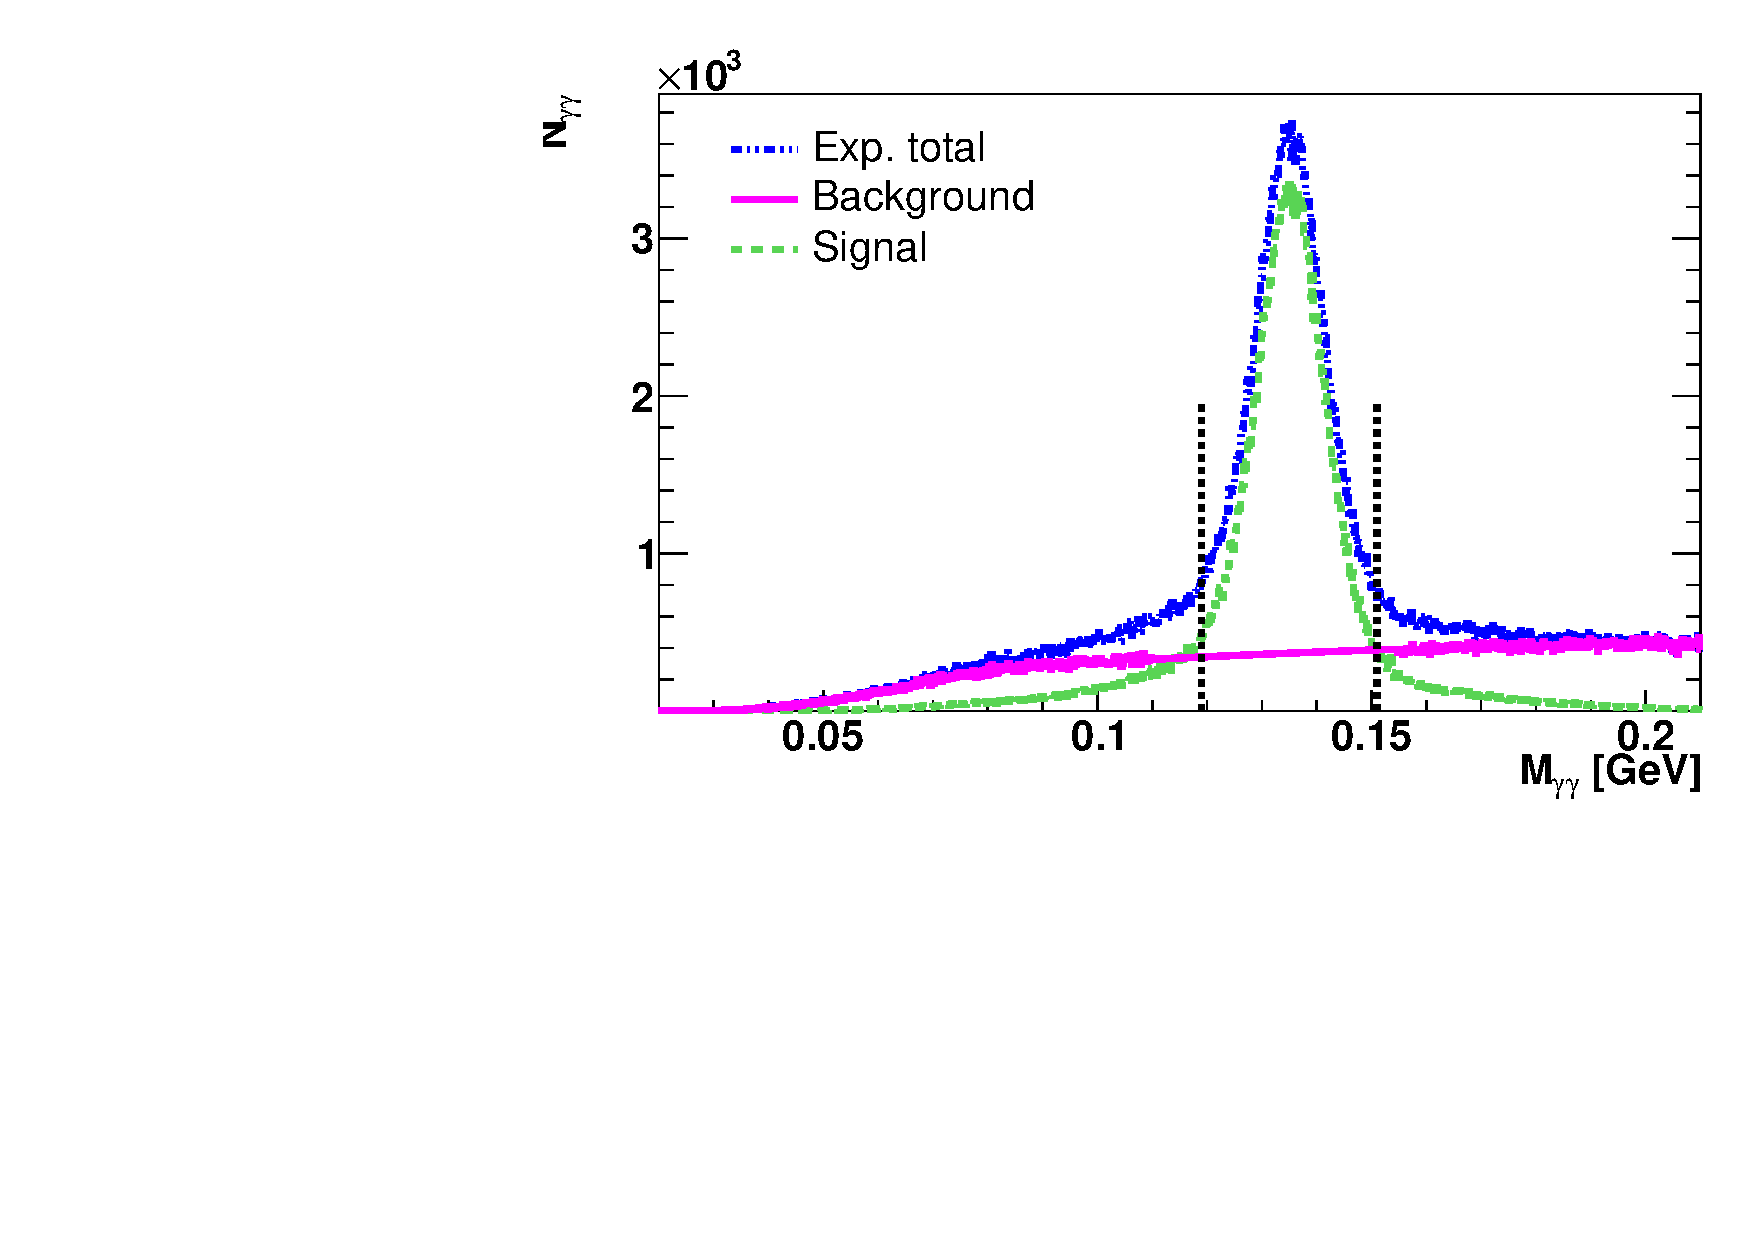
\includegraphics[width=.48\textwidth,natwidth=600,natheight=400]{figure_dataselection/pi0_fit_Pt_2.pdf}}
  \subfigure[$P_t$ bin 3 (0.5 GeV $<P_t<$ 3 GeV)]{\label{fig:pi0fitpt3}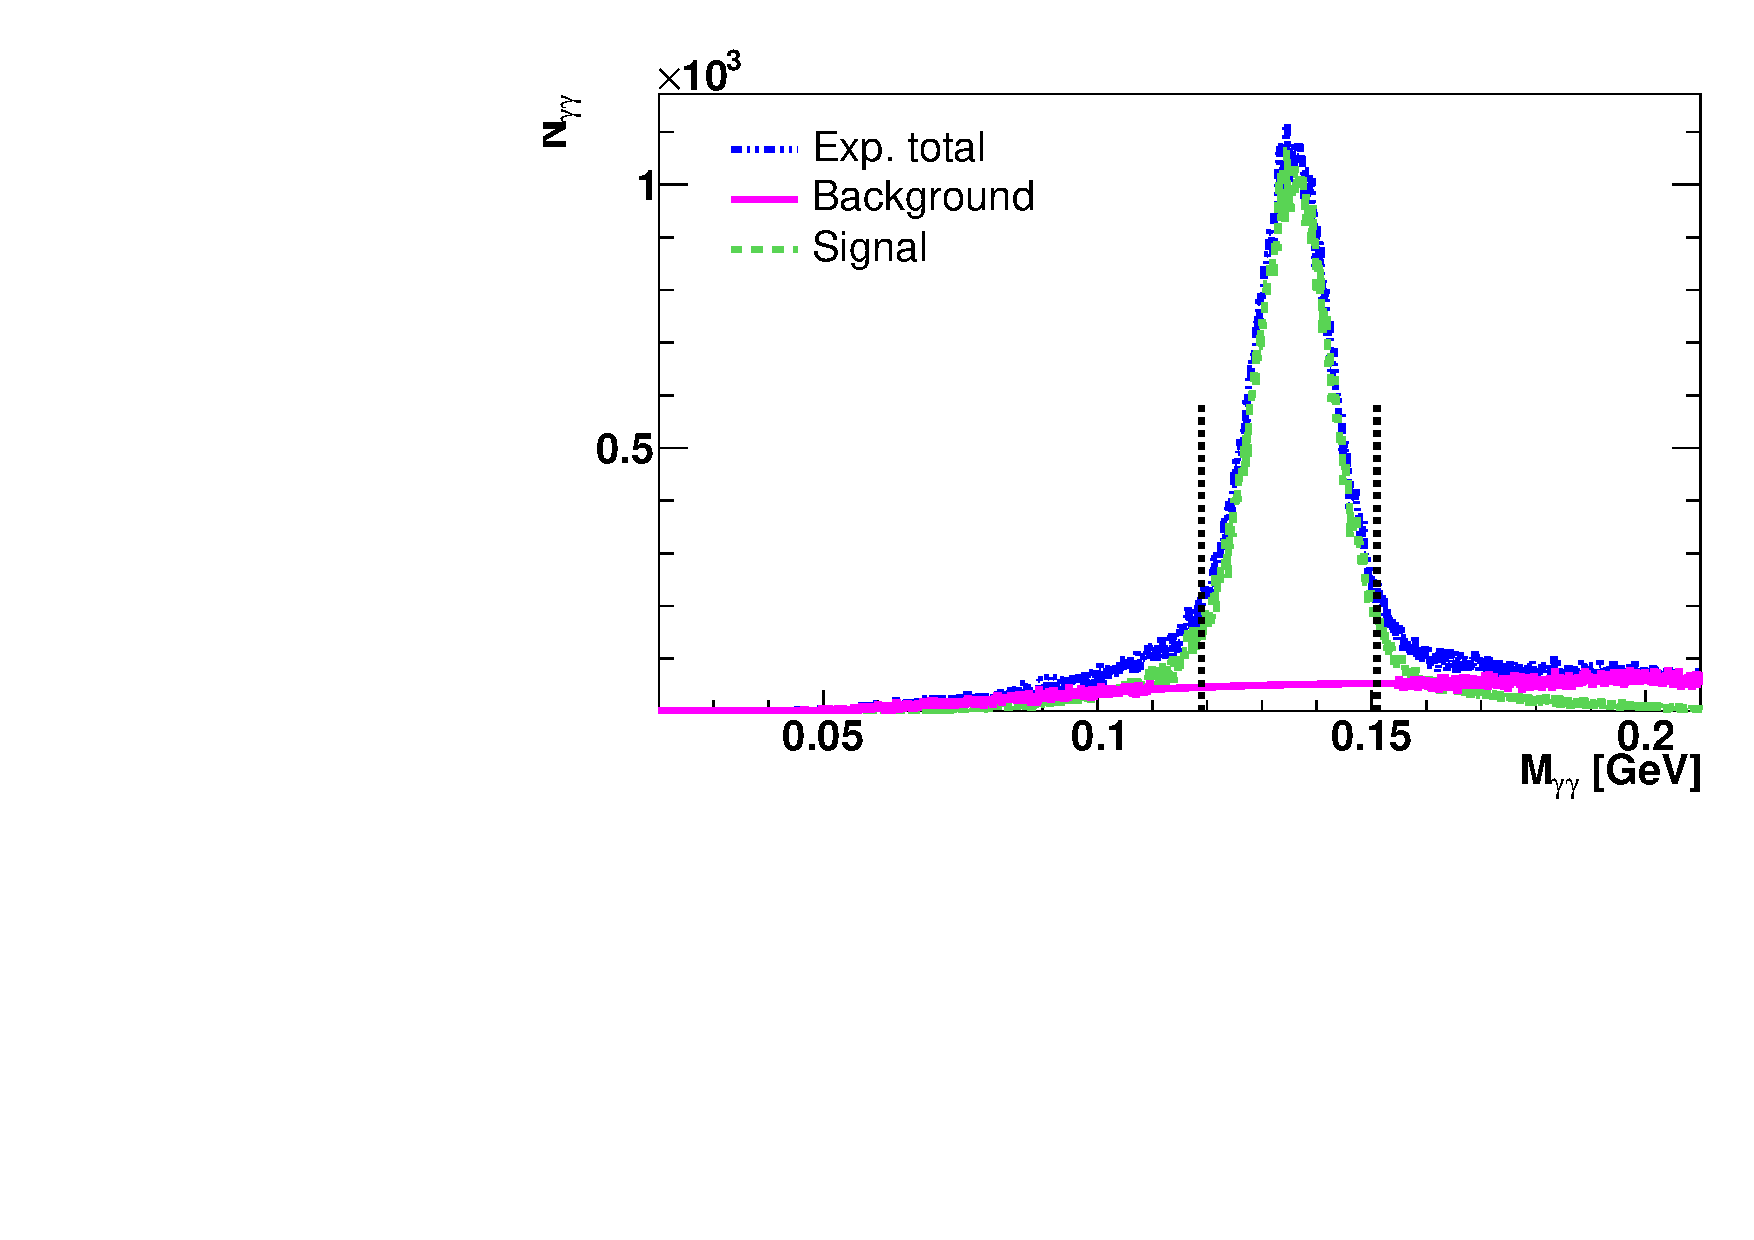
\includegraphics[width=.48\textwidth,natwidth=600,natheight=400]{figure_dataselection/pi0_fit_Pt_3.pdf}}
  \caption[Invariant-mass fit for $\pi^0$ with MC-based background, \(P_{t}\) bins]{Invariant-mass fit for $\pi^0$ with MC-based background, \(P_{t}\) bins (systematic check). Fit method as described in Section~\ref{sec:pi0fitsection}. Magenta line is the background and green dashed line is the signal.}
  \label{fig:pi0ptfit2}
\end{figure}

\begin{figure}[H]
  \centering     \tiny
  \subfigure[$z$ bin 0 ($0.1<z<0.2$)]{\label{fig:pi0fitz1}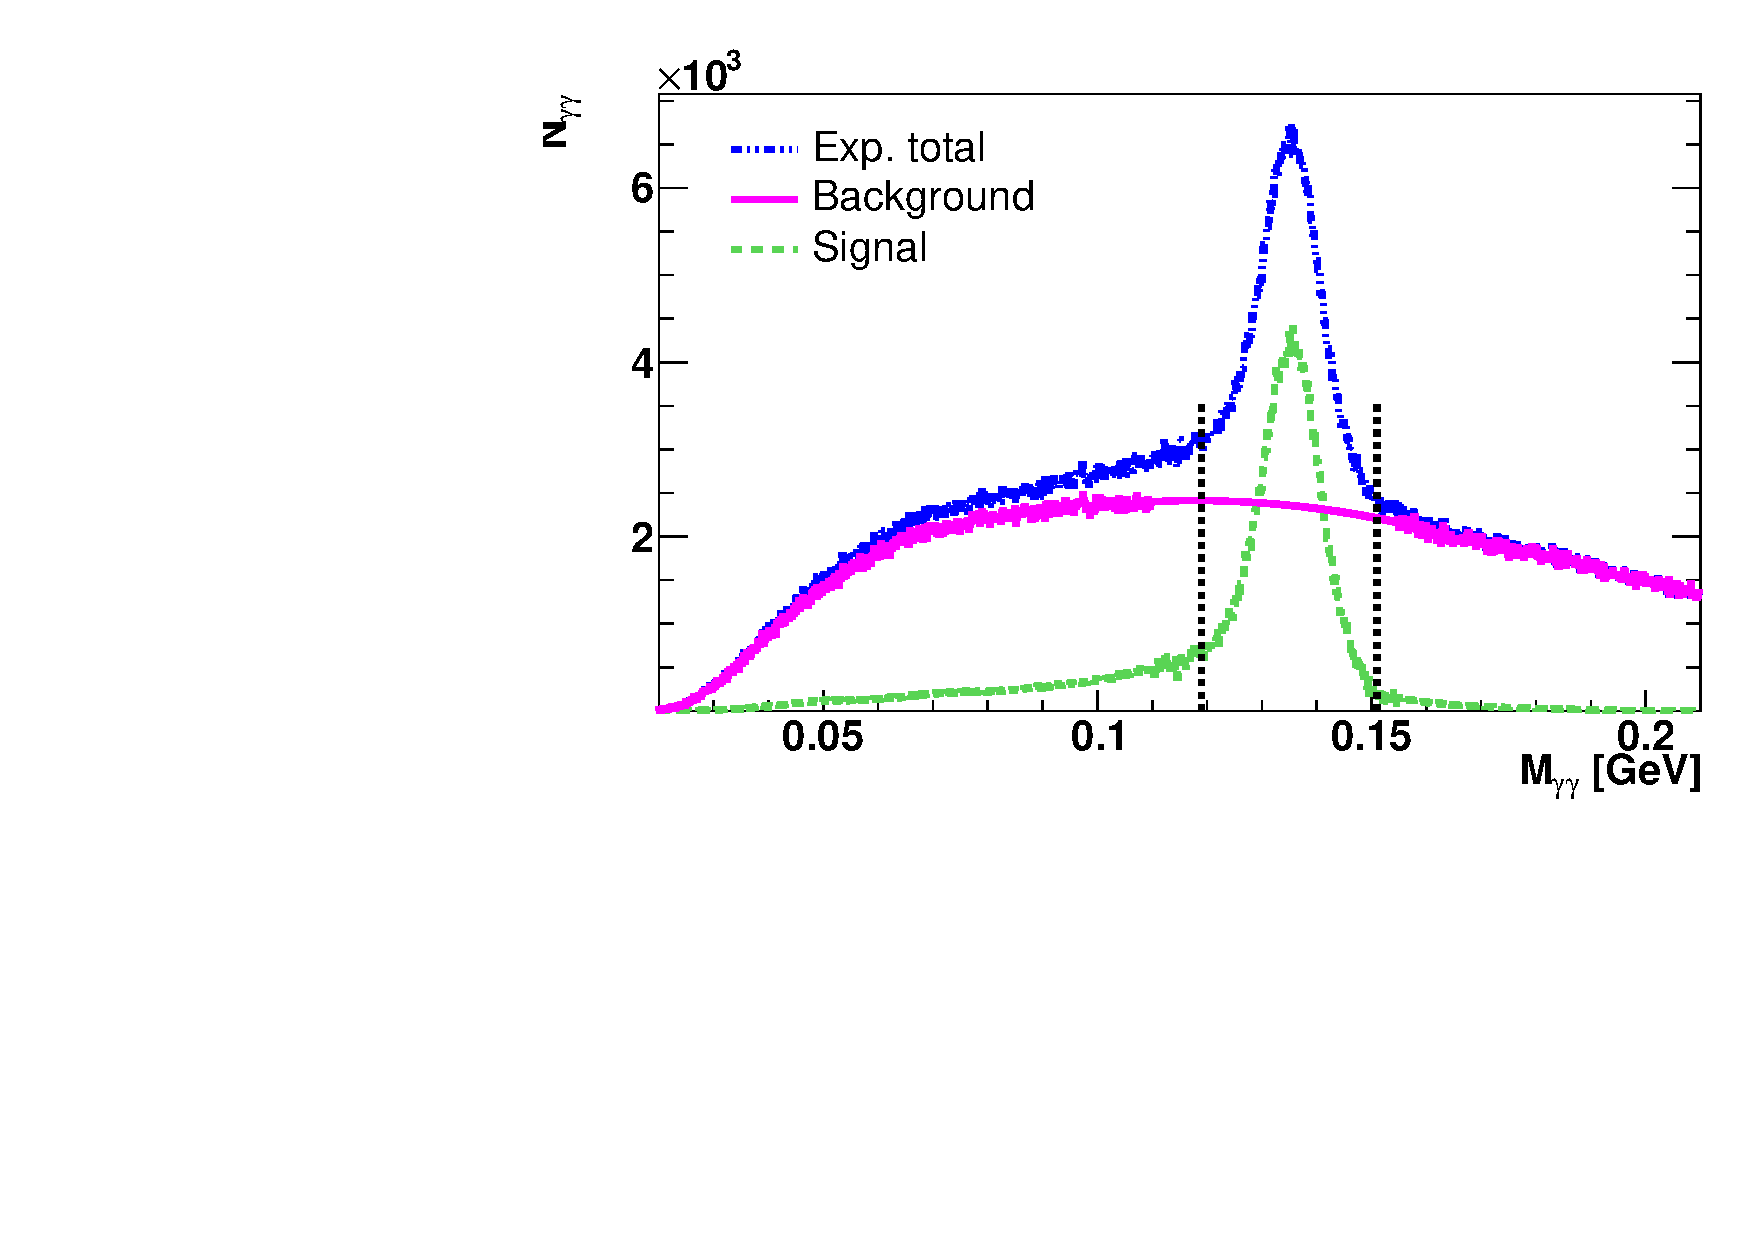
\includegraphics[width=.48\textwidth,natwidth=600,natheight=400]{figure_dataselection/pi0_fit_Z_0.pdf}}
  \subfigure[$z$ bin 1 ($0.2<z<0.3$)]{\label{fig:pi0fitz2}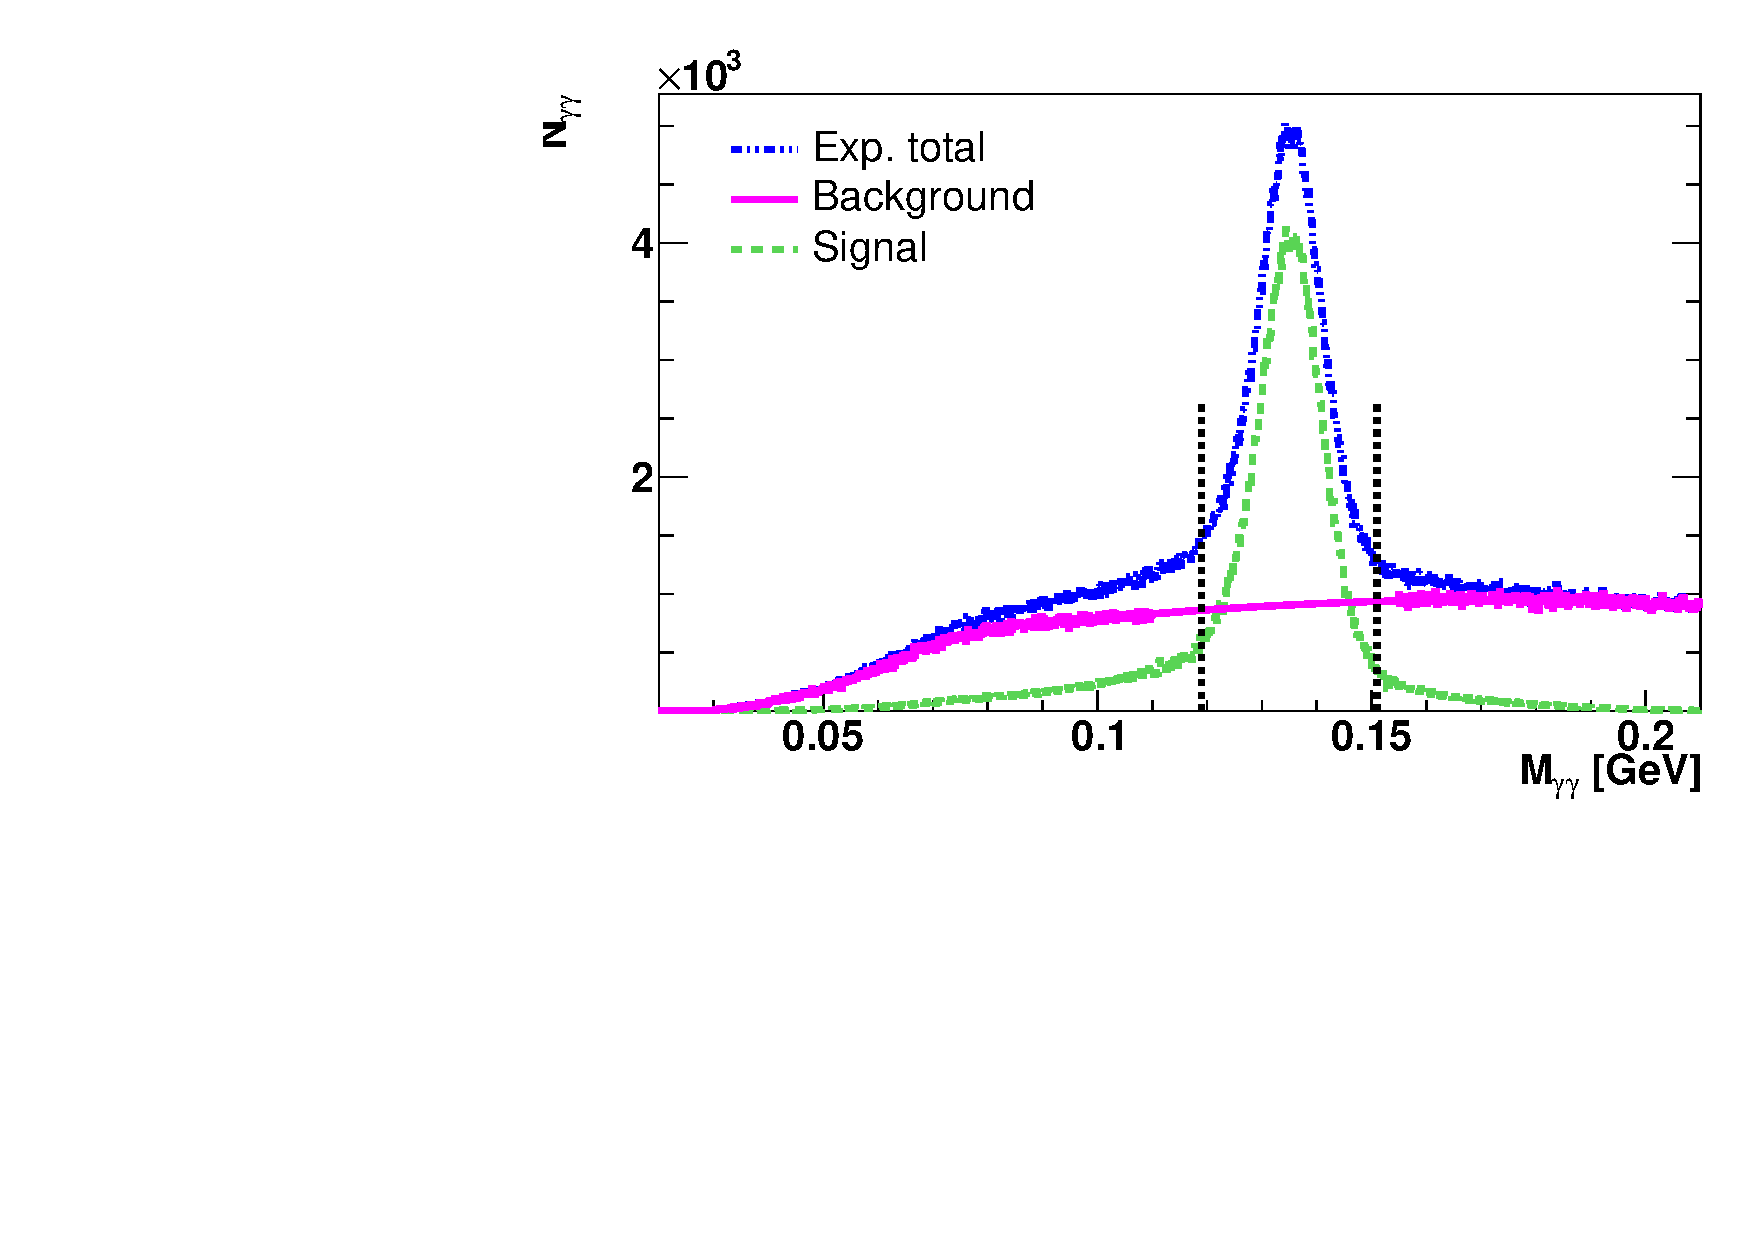
\includegraphics[width=.48\textwidth,natwidth=600,natheight=400]{figure_dataselection/pi0_fit_Z_1.pdf}}
  \subfigure[$z$ bin 2 ($0.3<z<0.4$)]{\label{fig:pi0fitz3}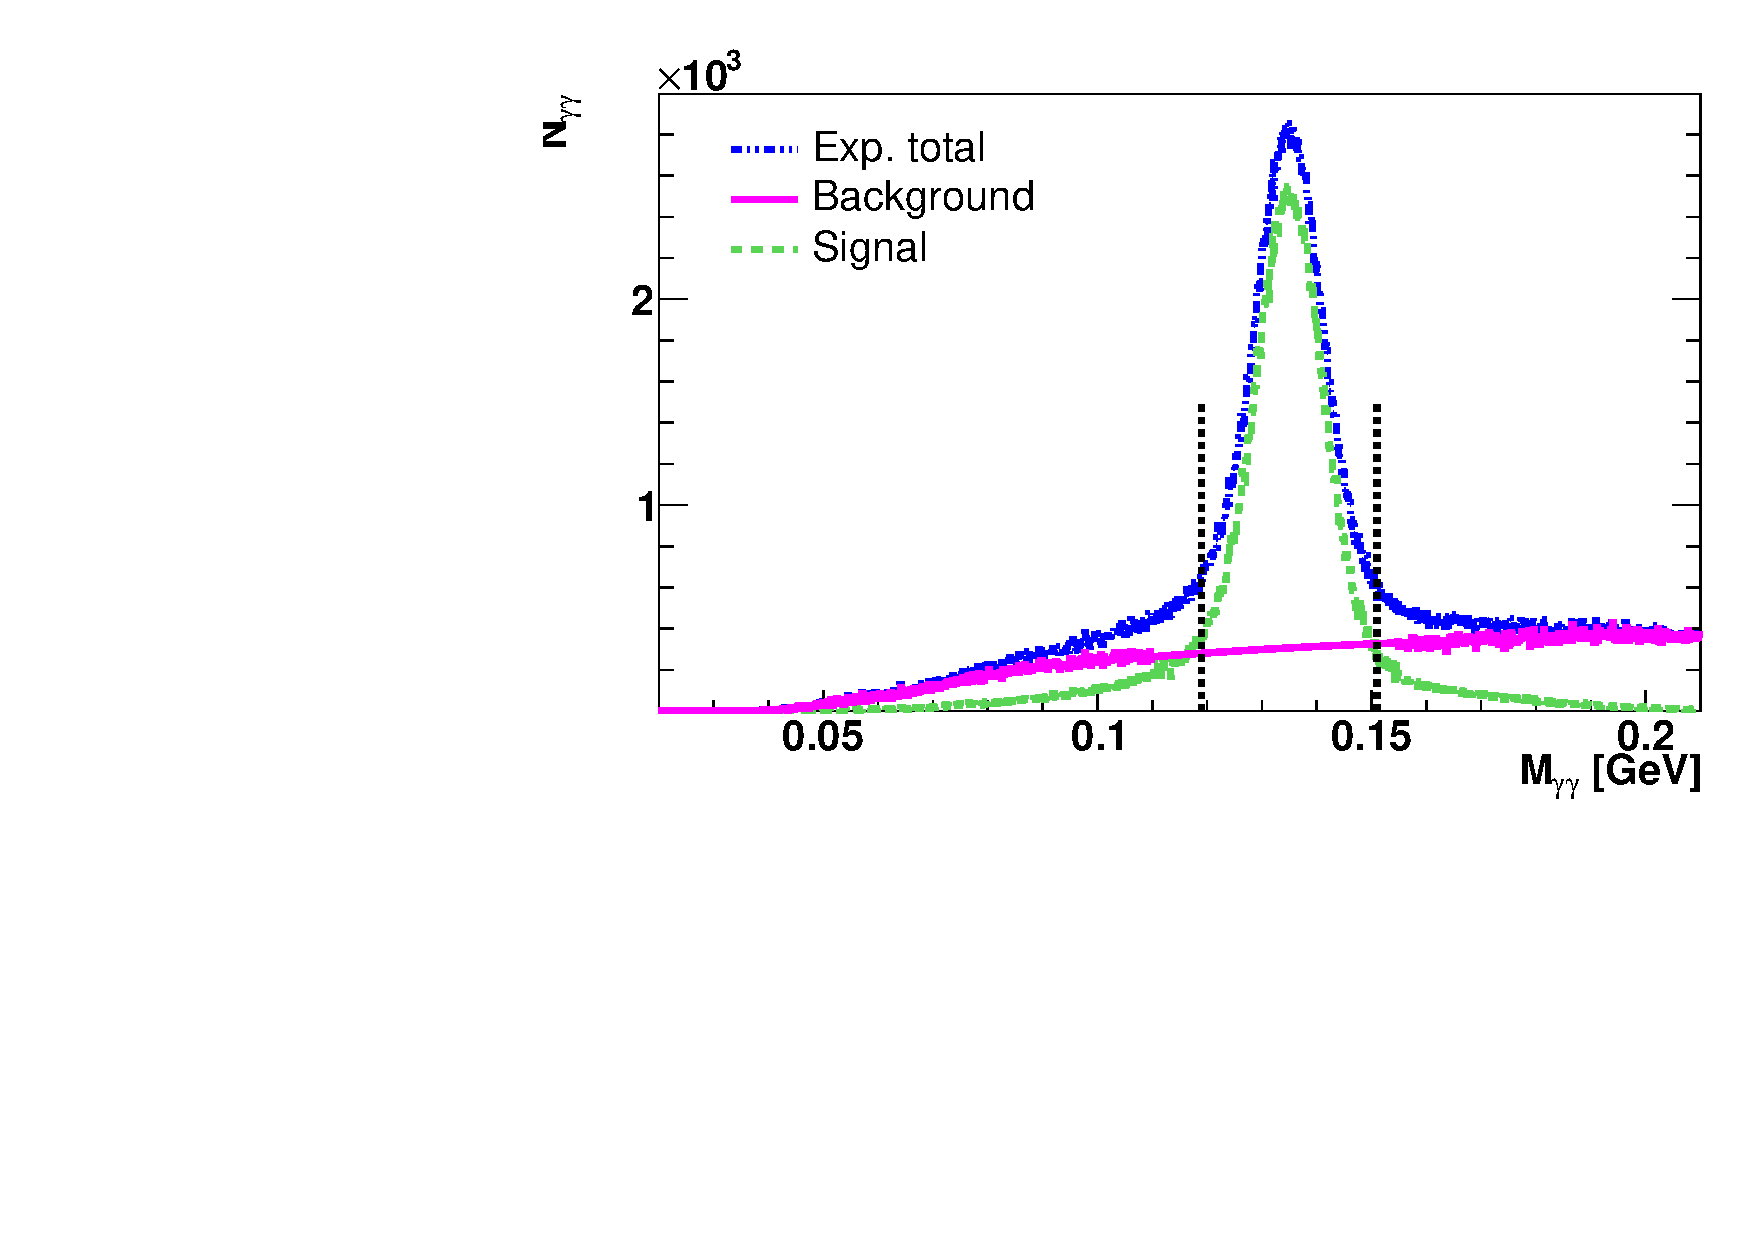
\includegraphics[width=.48\textwidth,natwidth=600,natheight=400]{figure_dataselection/pi0_fit_Z_2.pdf}}
  \subfigure[$z$ bin 3 ($0.4<z<0.5$)]{\label{fig:pi0fitz4}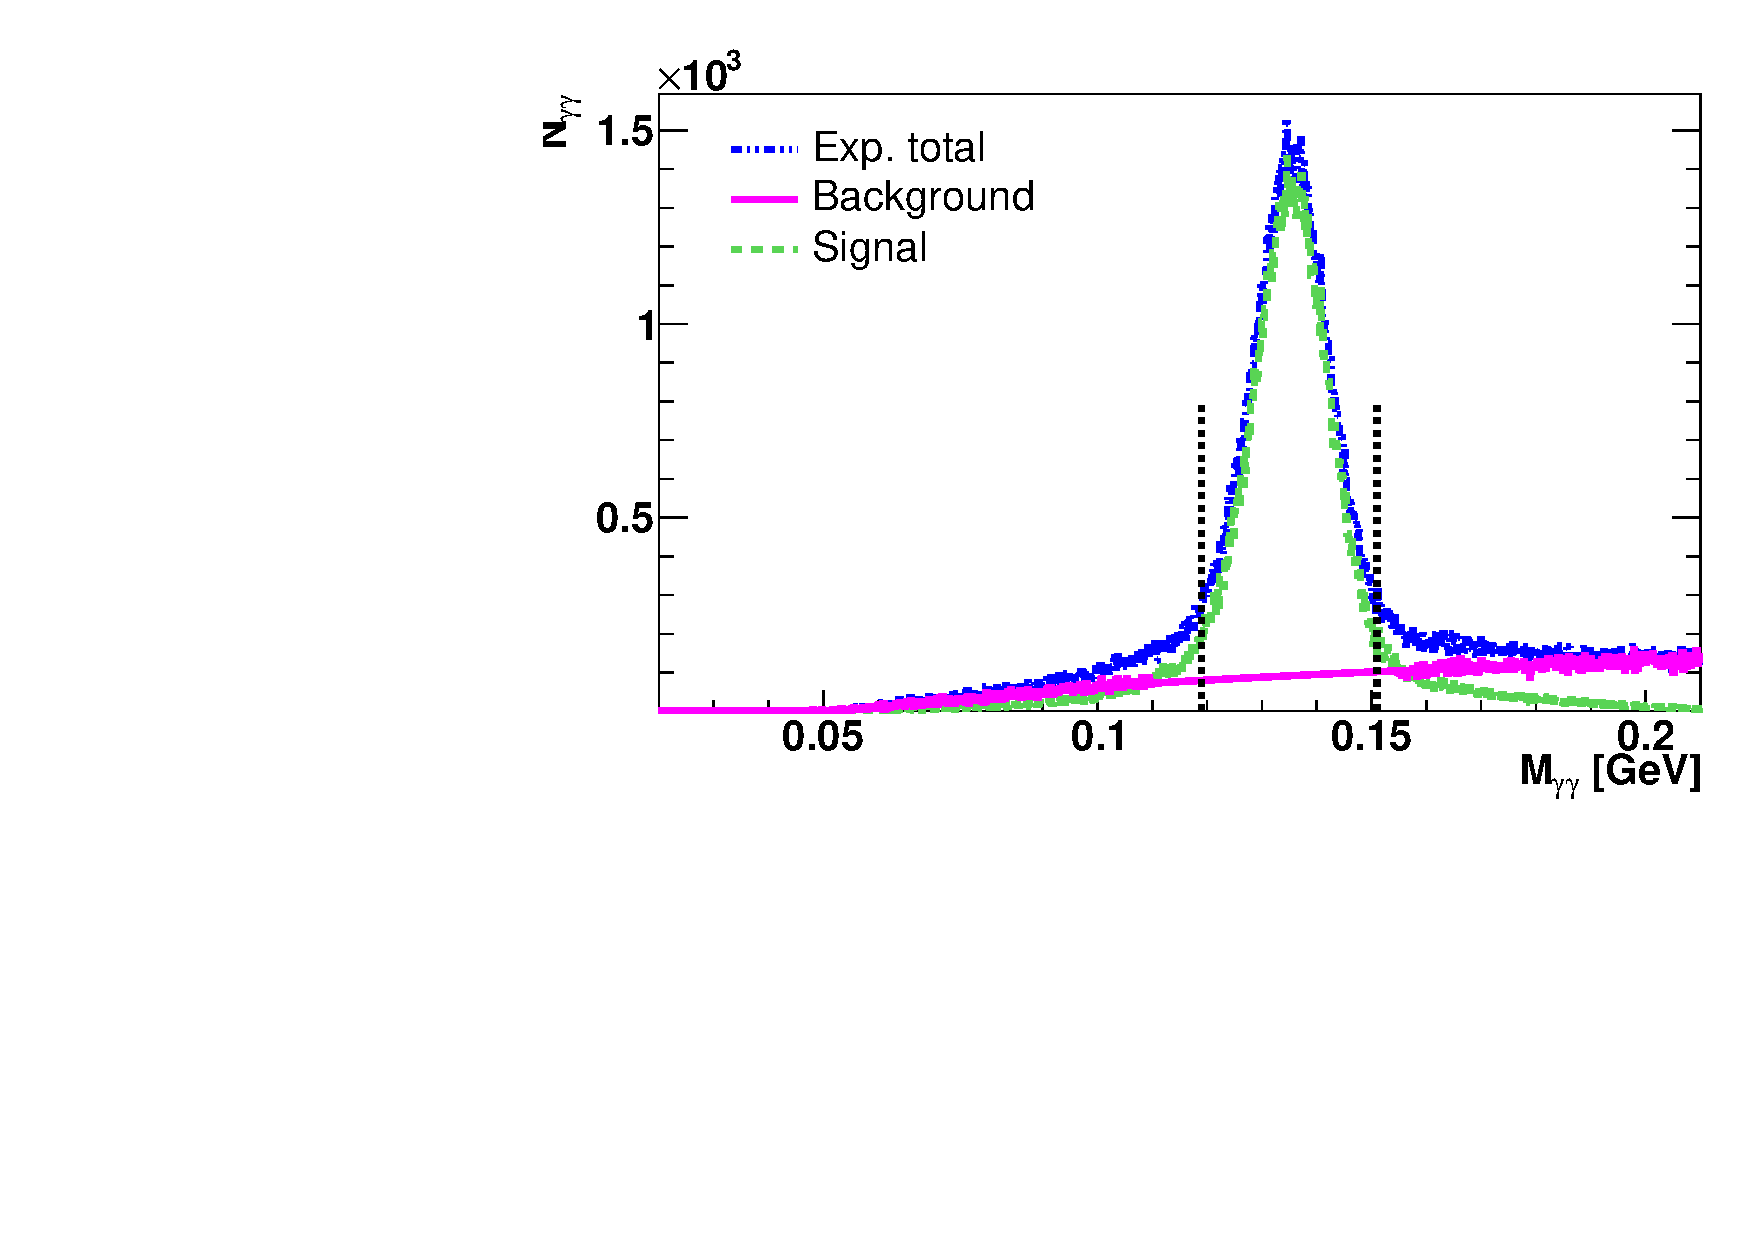
\includegraphics[width=.48\textwidth,natwidth=600,natheight=400]{figure_dataselection/pi0_fit_Z_3.pdf}}
  \subfigure[$z$ bin 4 ($0.5<z<0.6$)]{\label{fig:pi0fitz5}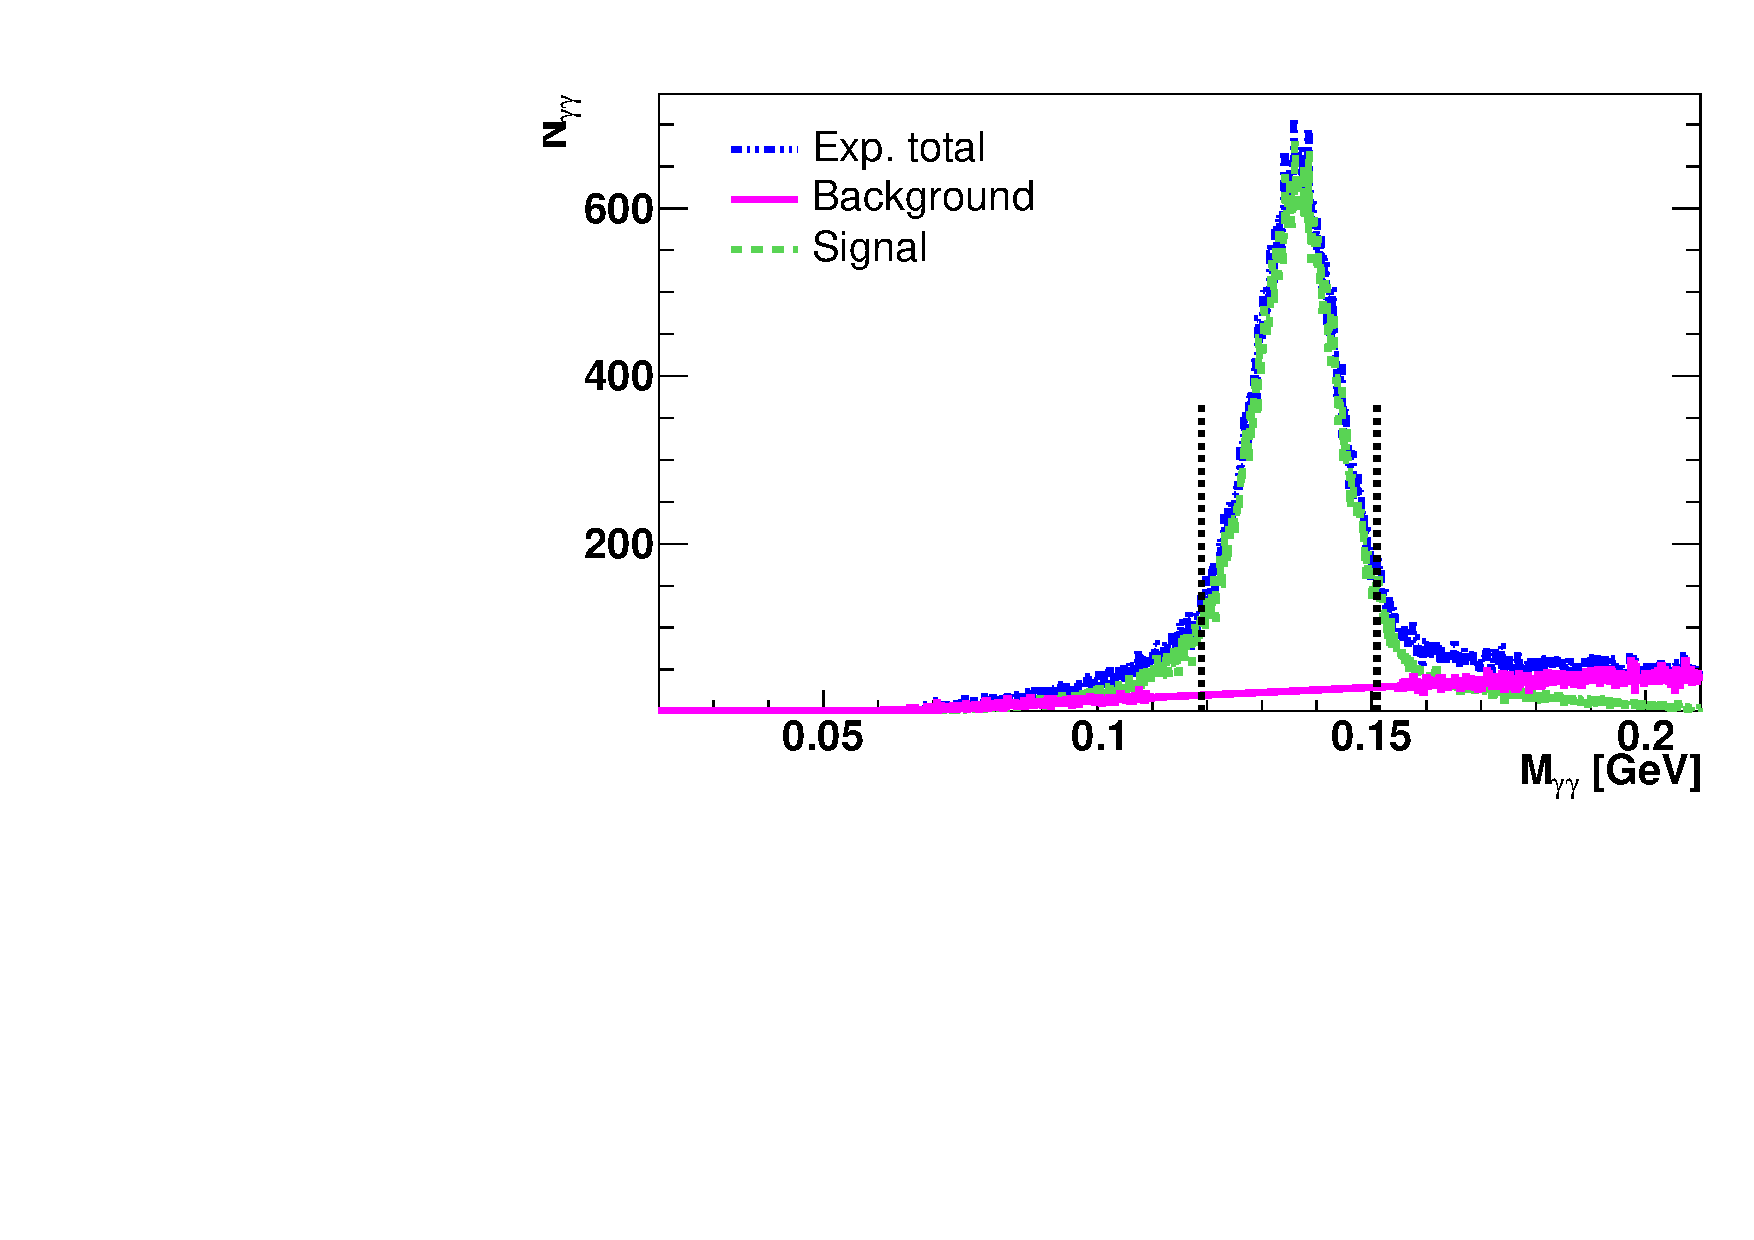
\includegraphics[width=.48\textwidth,natwidth=600,natheight=400]{figure_dataselection/pi0_fit_Z_4.pdf}}
  \subfigure[$z$ bin 5 ($0.6<z<0.7$)]{\label{fig:pi0fitz6}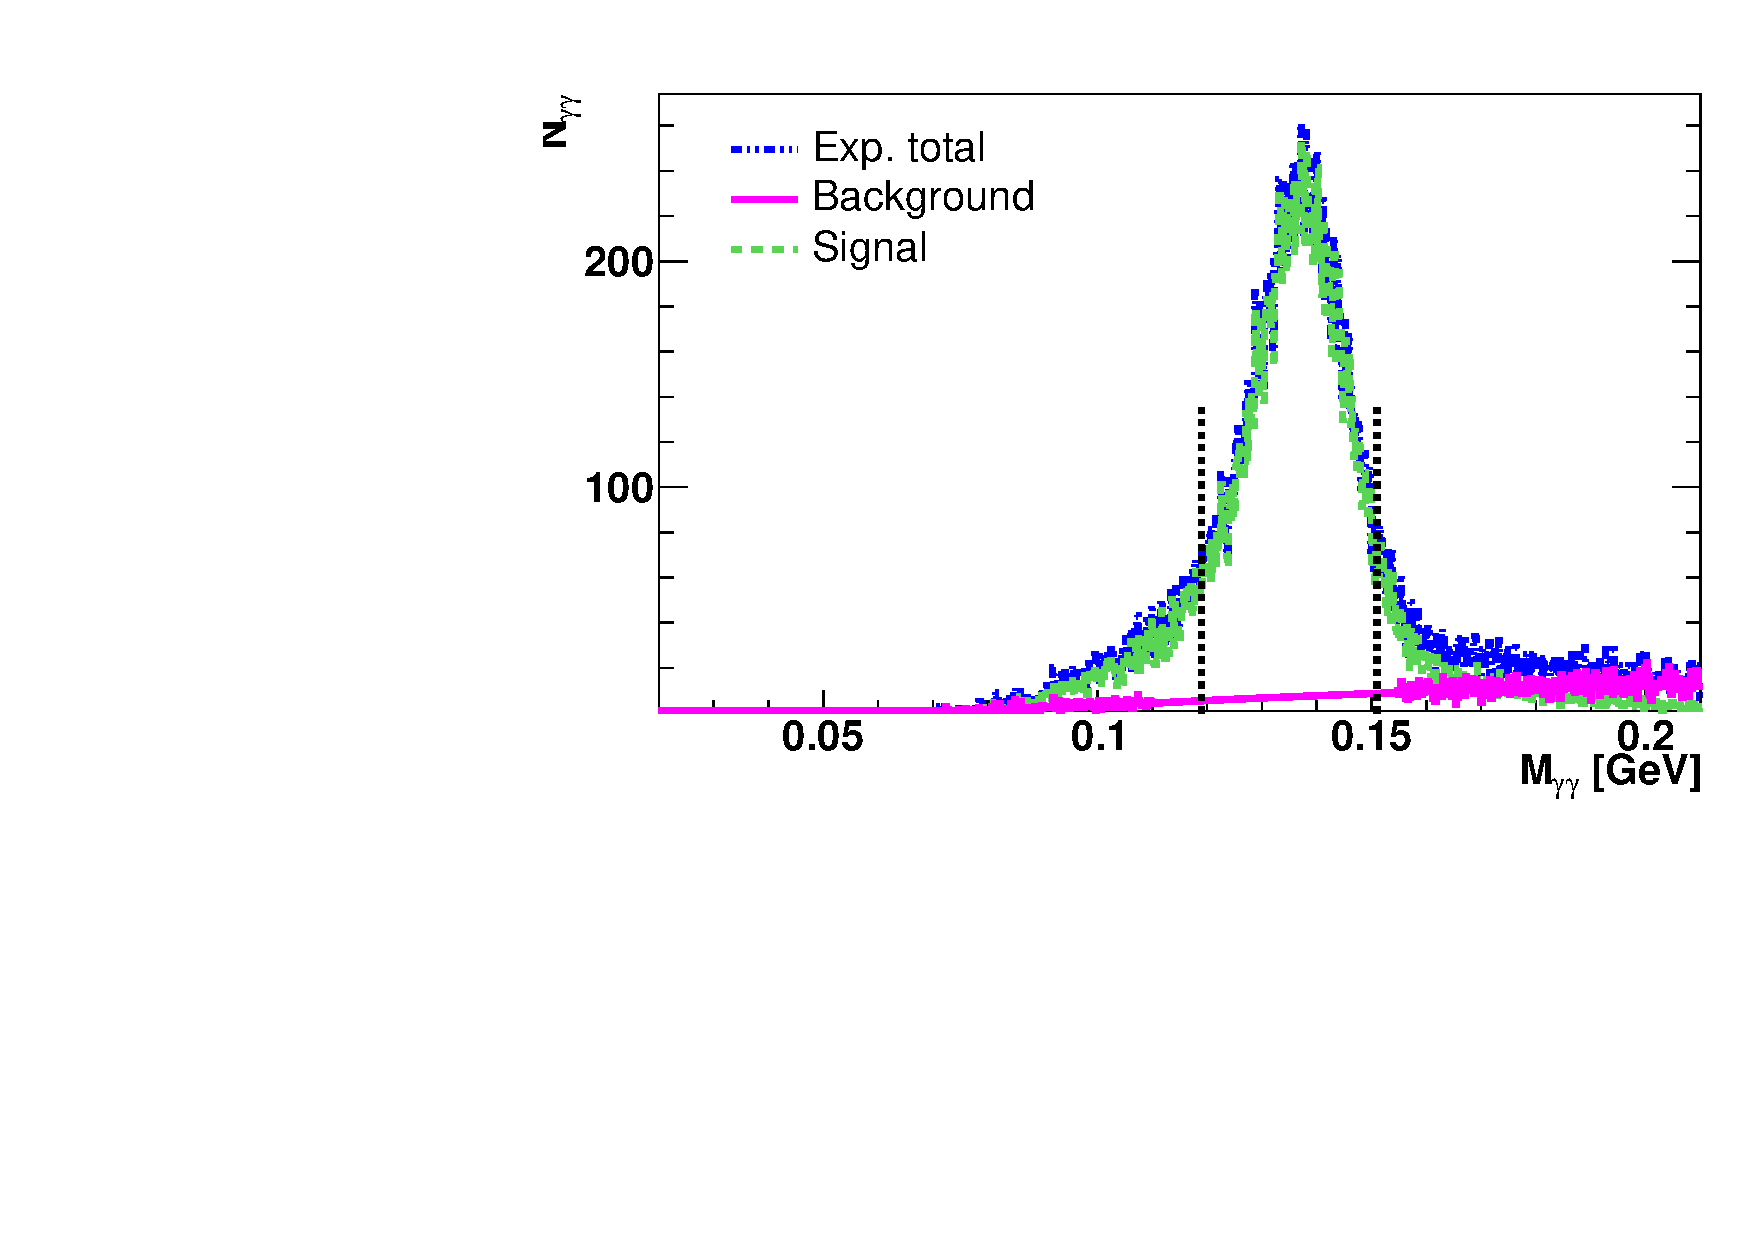
\includegraphics[width=.48\textwidth,natwidth=600,natheight=400]{figure_dataselection/pi0_fit_Z_5.pdf}}
  \subfigure[$z$ bin 6 ($0.7<z<1$)]{\label{fig:pi0fitz7}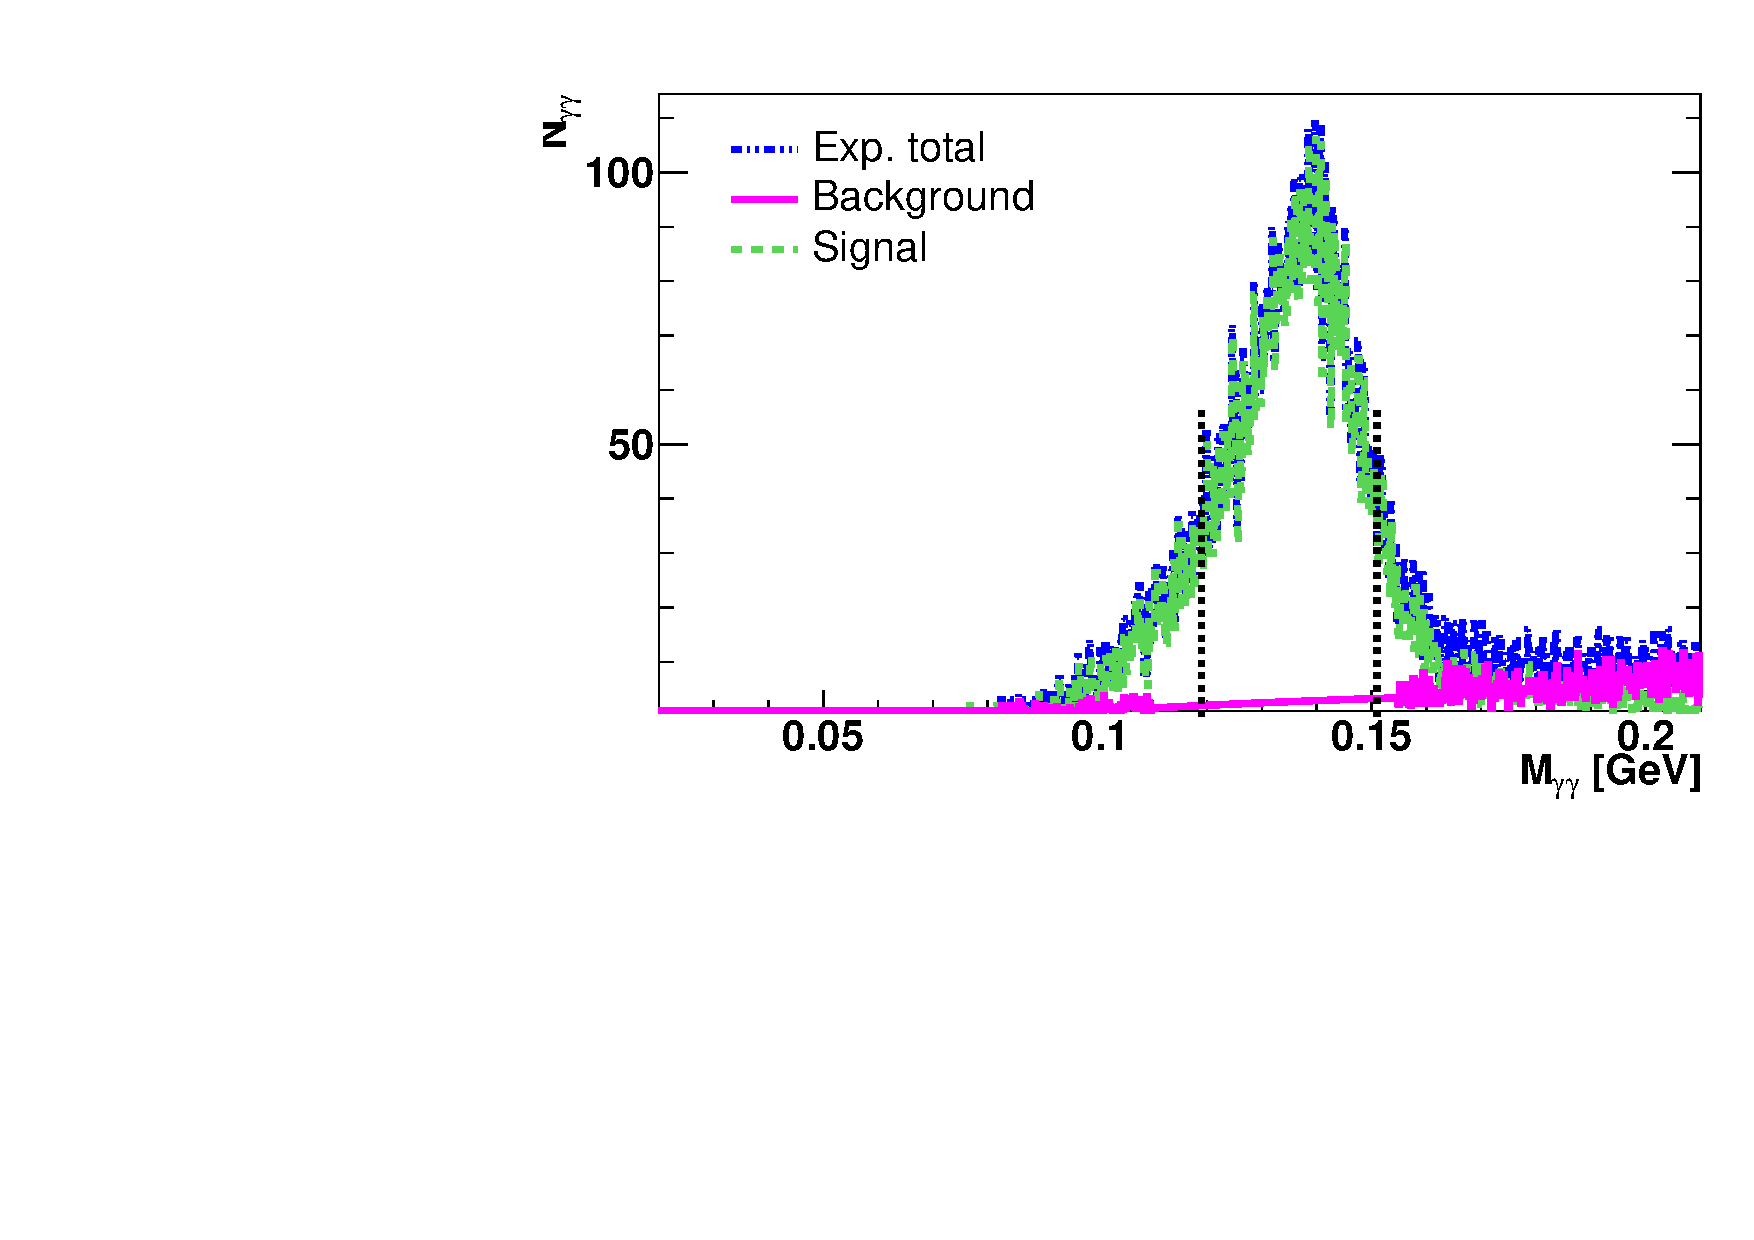
\includegraphics[width=.48\textwidth,natwidth=600,natheight=400]{figure_dataselection/pi0_fit_Z_6.pdf}}
\label{fig:pi0zfit2}
\caption[Invariant-mass fit for $\pi^0$ with MC-based background, \(z\) bins]{Invariant-mass fit for $\pi^0$ with MC-based background, \(z\) bins (systematic check). Fit method as described in Section~\ref{sec:pi0fitsection}. Magenta line is the background and green dashed line is the signal.}
\end{figure}


\subsubsection{\texorpdfstring{Invariant-mass fits for $\eta$ for all kinematic bins}{Invariant-mass fits for eta for all kinematic bins}}

\begin{figure}[H]
\ContinuedFloat*
 \centering     
 \subfigure[$z$ bin 2 ($0.3<z<0.4$)]{\label{fig:etafitz7}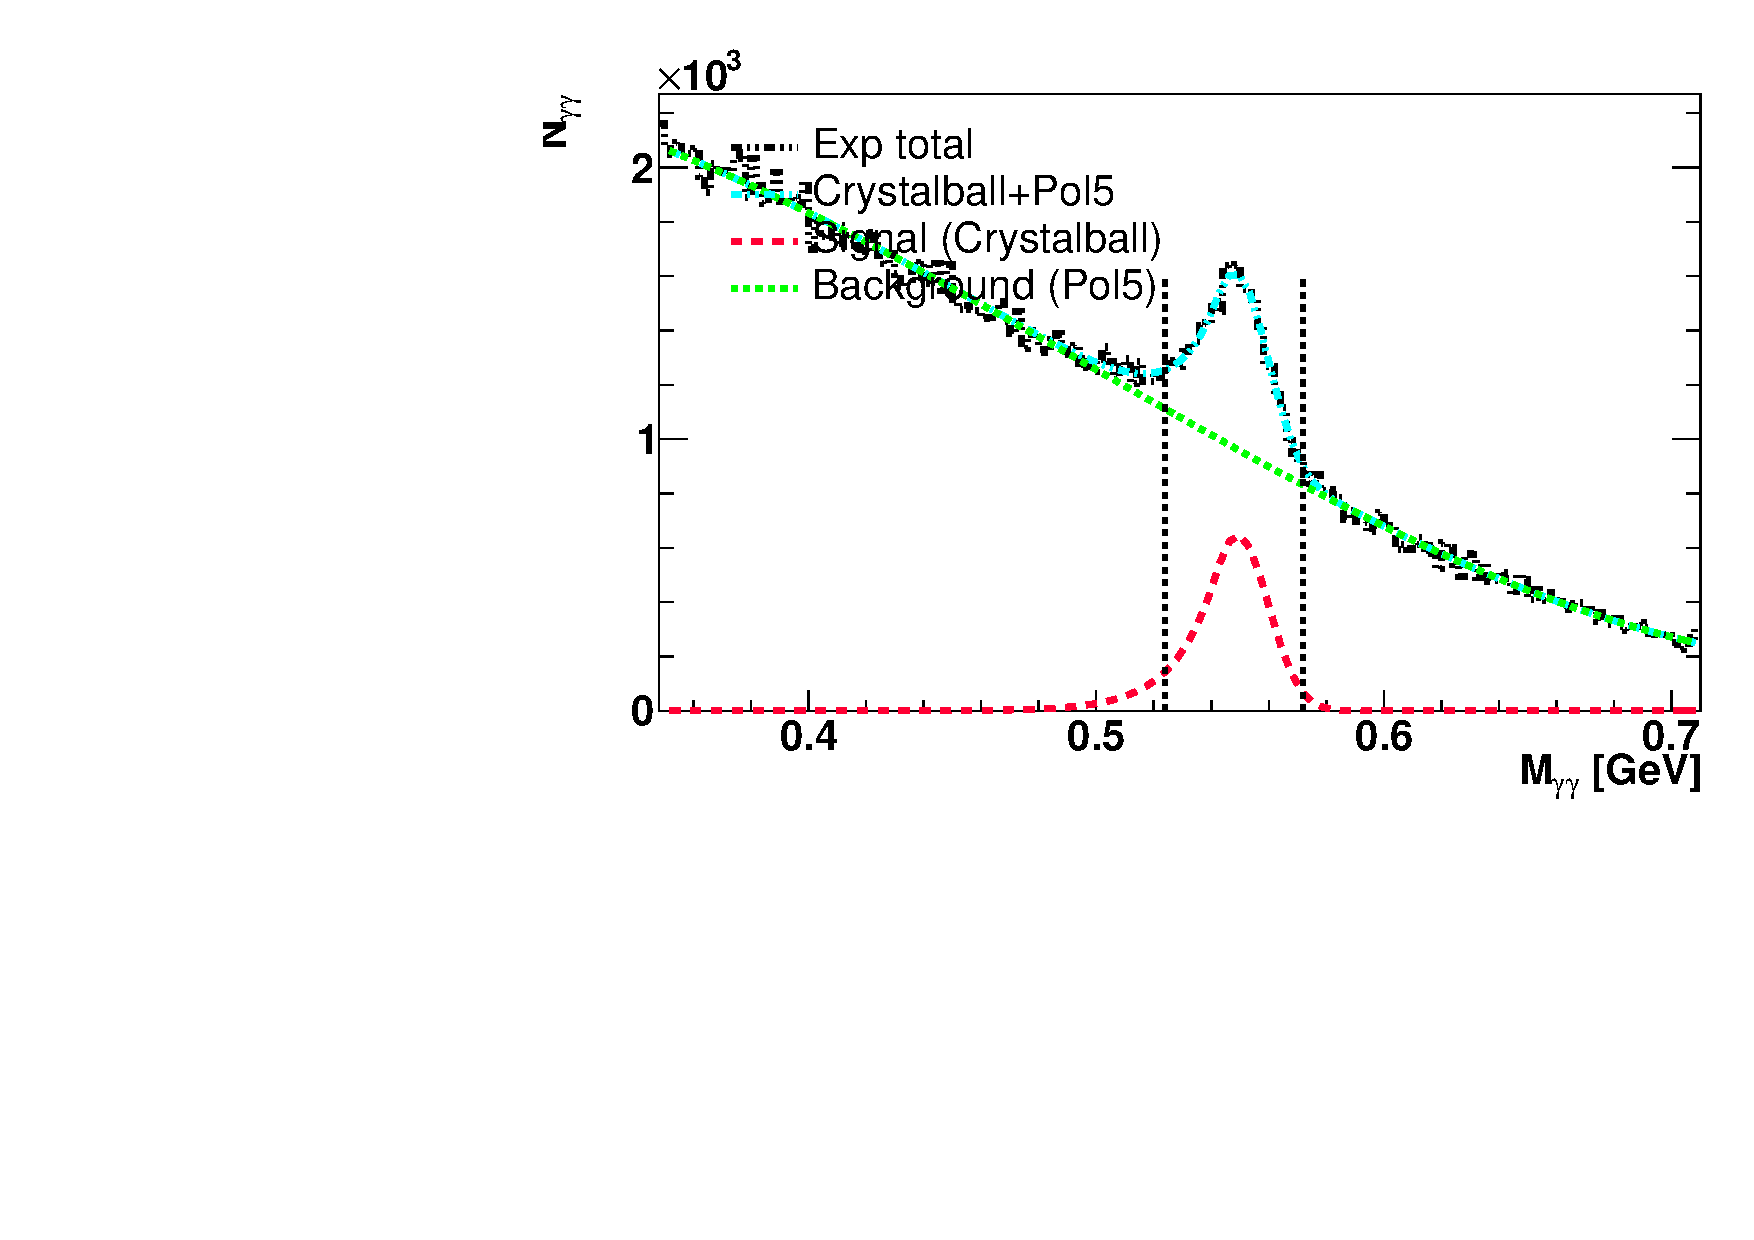
\includegraphics[width=.48\textwidth,natwidth=600,natheight=400]{figure_dataselection/eta_fitall_Z_2.pdf}}
 \subfigure[$z$ bin 2 ($0.3<z<0.4$)]{\label{fig:etafitz42}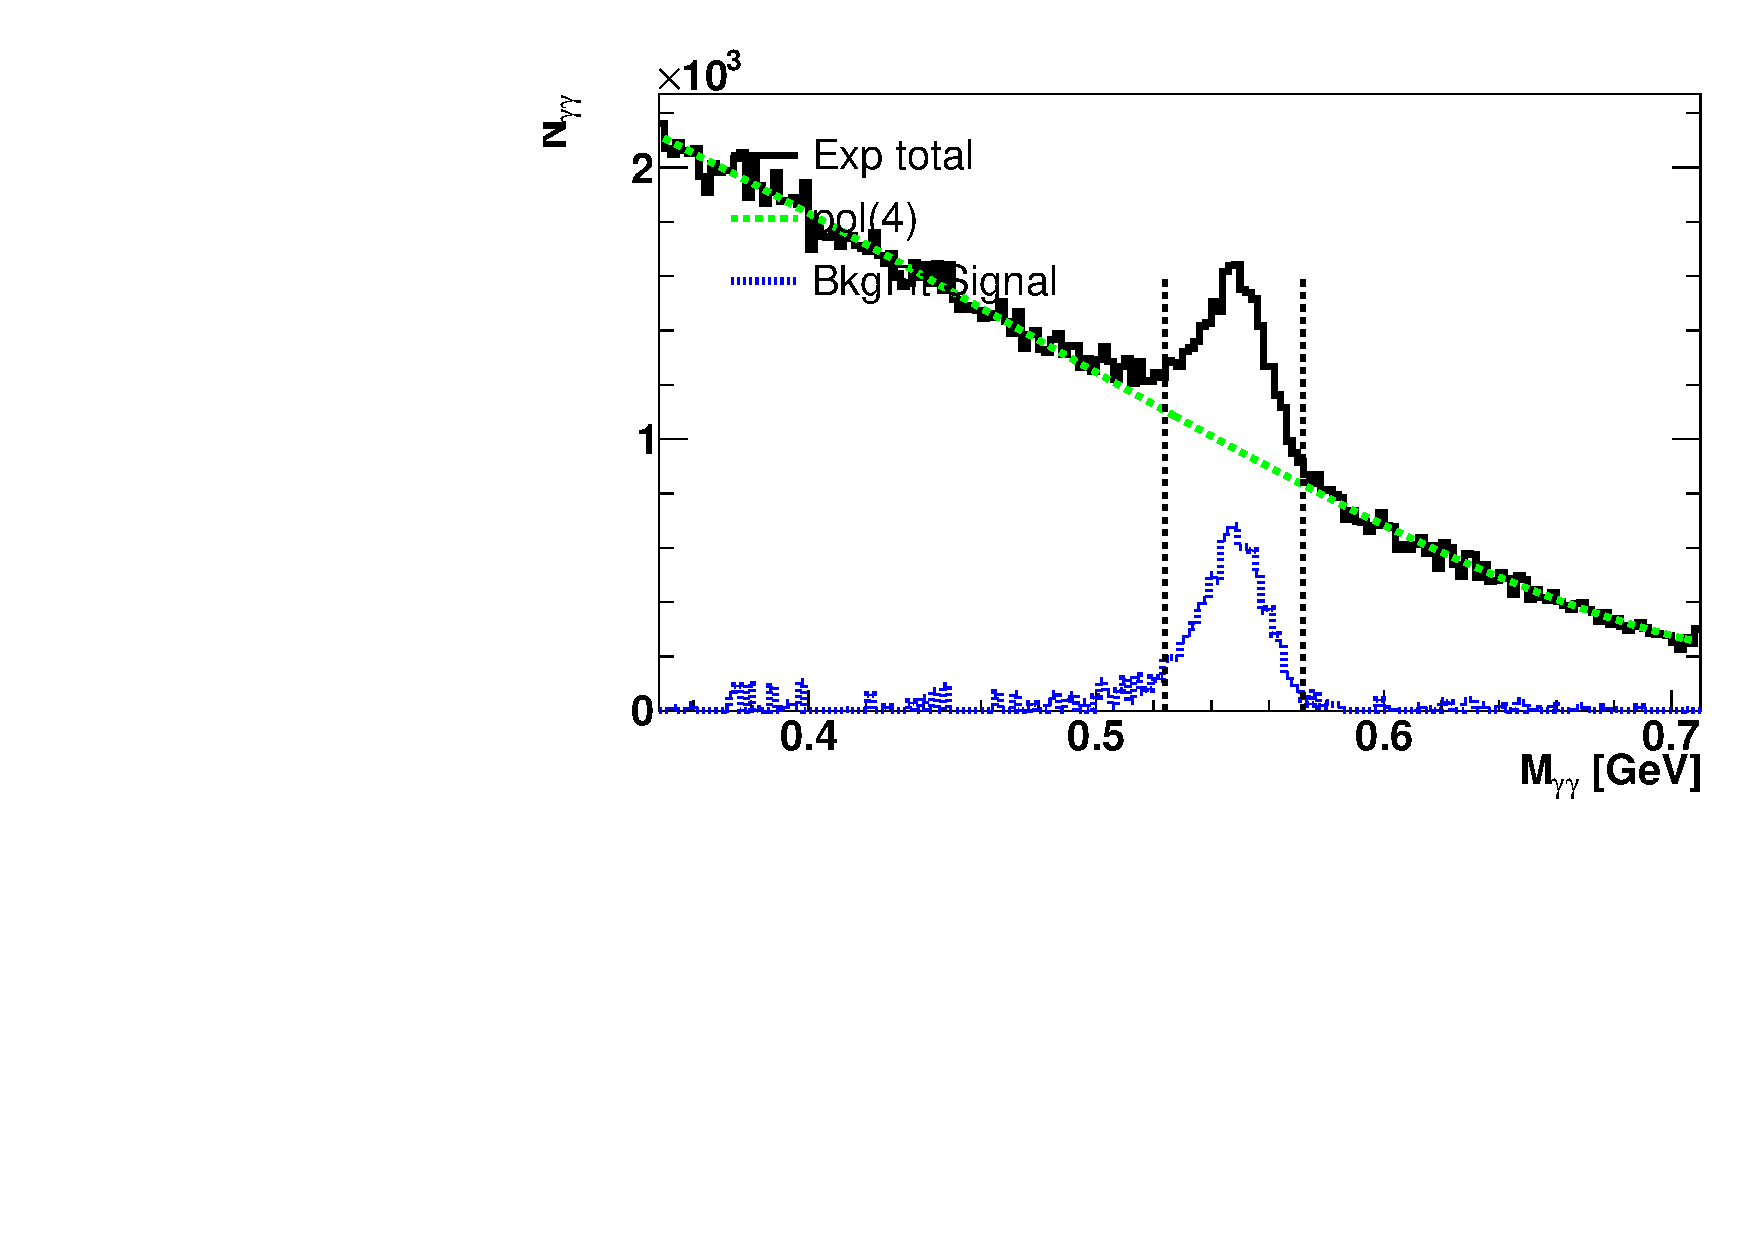
\includegraphics[width=.48\textwidth,natwidth=600,natheight=400]{figure_dataselection/eta_fitbkg_Z_2.pdf}}
 \subfigure[$z$ bin 3 ($0.4<z<0.5$)]{\label{fig:etafitz7}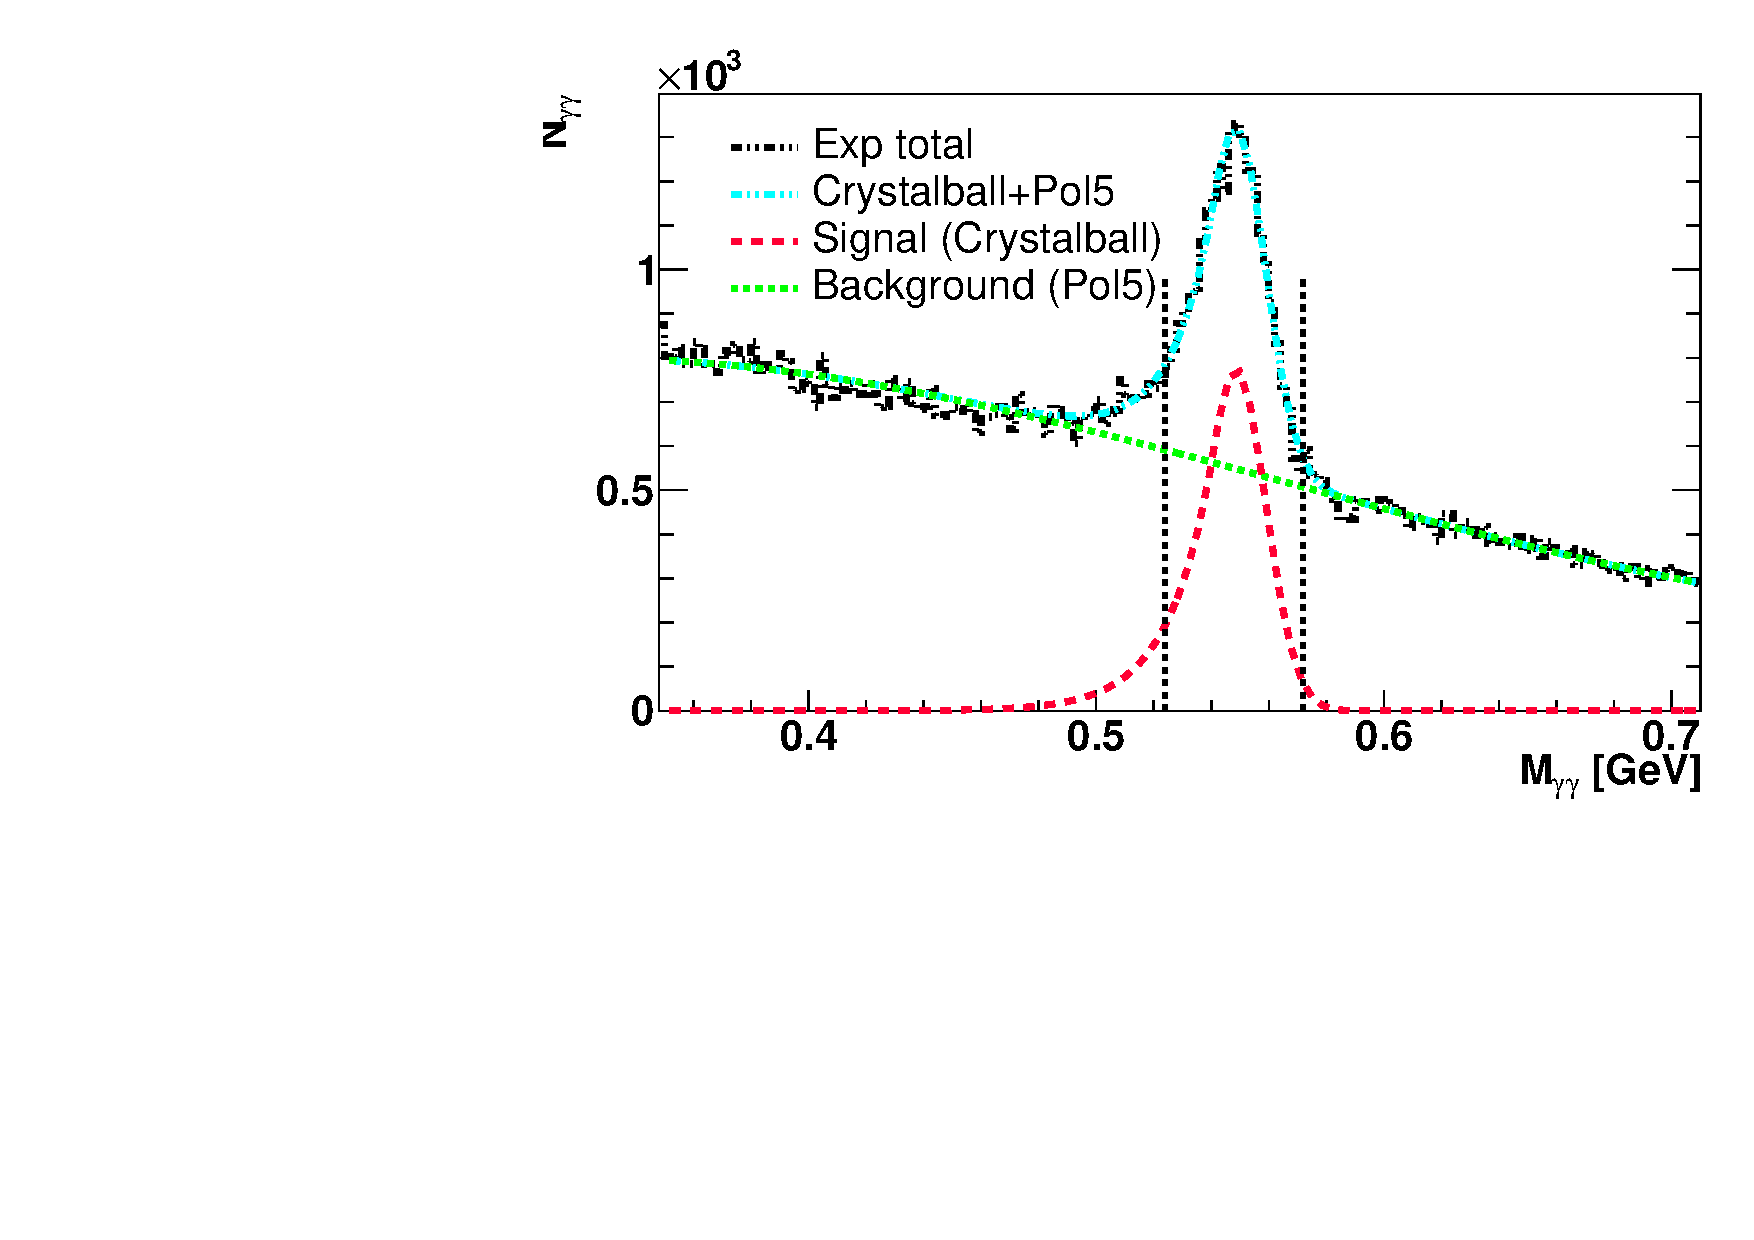
\includegraphics[width=.48\textwidth,natwidth=600,natheight=400]{figure_dataselection/eta_fitall_Z_3.pdf}}
 \subfigure[$z$ bin 3 ($0.4<z<0.5$)]{\label{fig:etafitz42}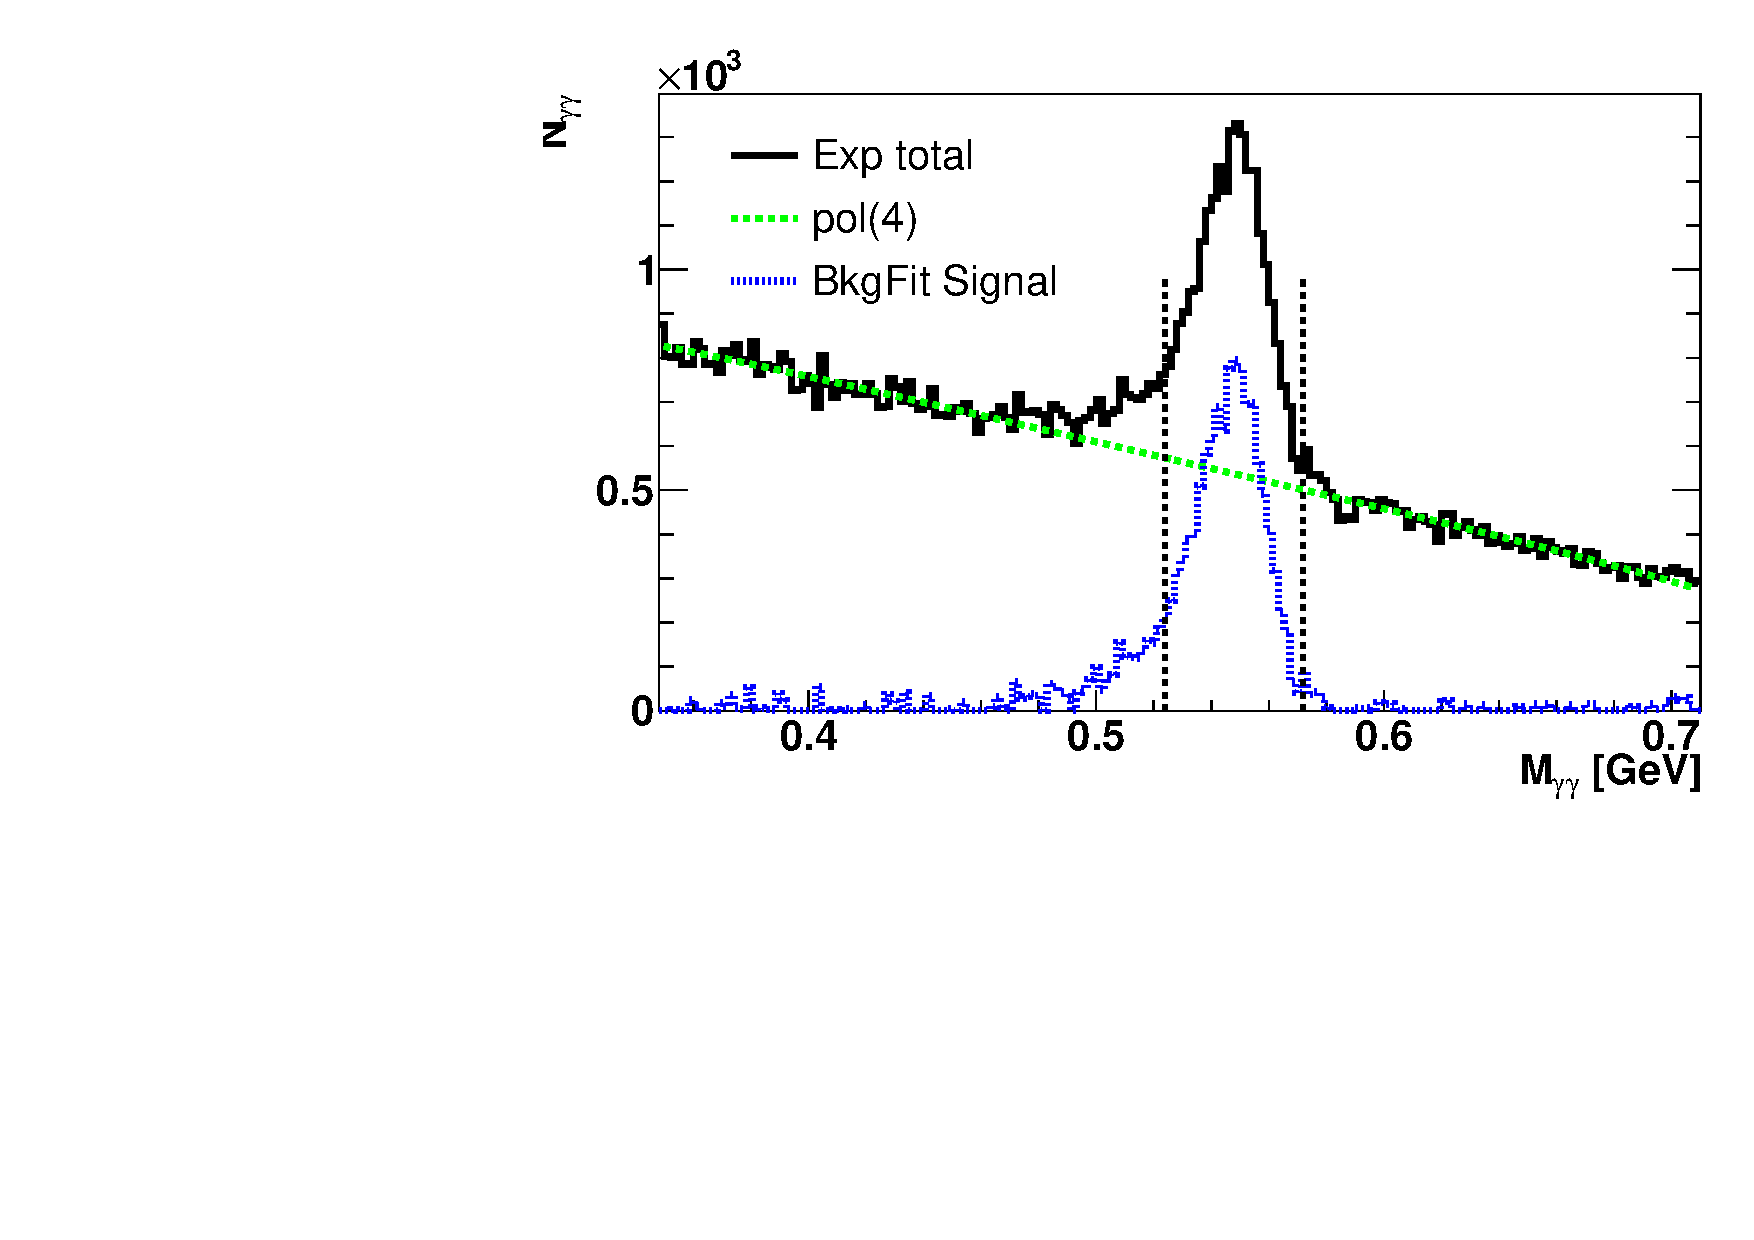
\includegraphics[width=.48\textwidth,natwidth=600,natheight=400]{figure_dataselection/eta_fitbkg_Z_3.pdf}}
 \subfigure[$z$ bin 4 ($0.5<z<0.6$)]{\label{fig:etafitz4}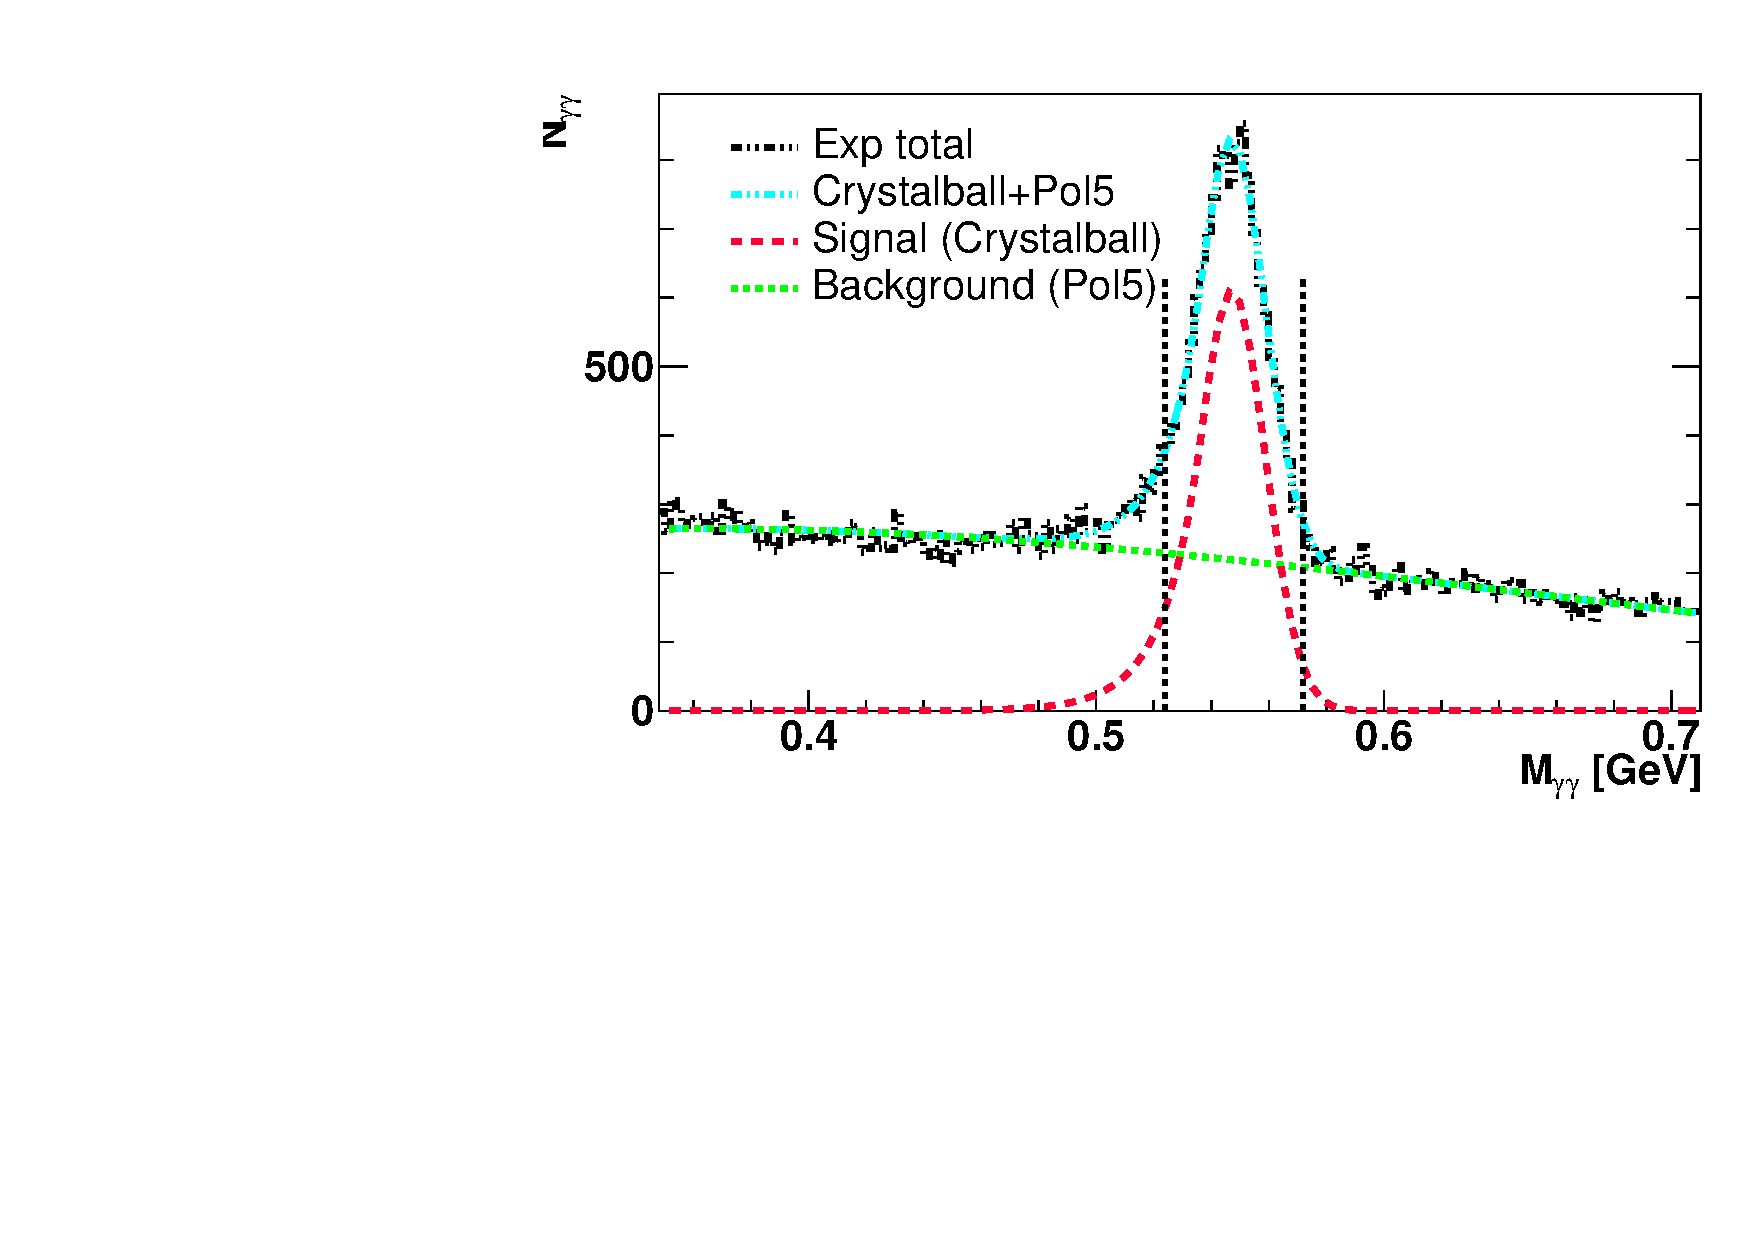
\includegraphics[width=.48\textwidth,natwidth=600,natheight=400]{figure_dataselection/eta_fitall_Z_4.pdf}}
 \subfigure[$z$ bin 4 ($0.5<z<0.6$)]{\label{fig:etafitz42}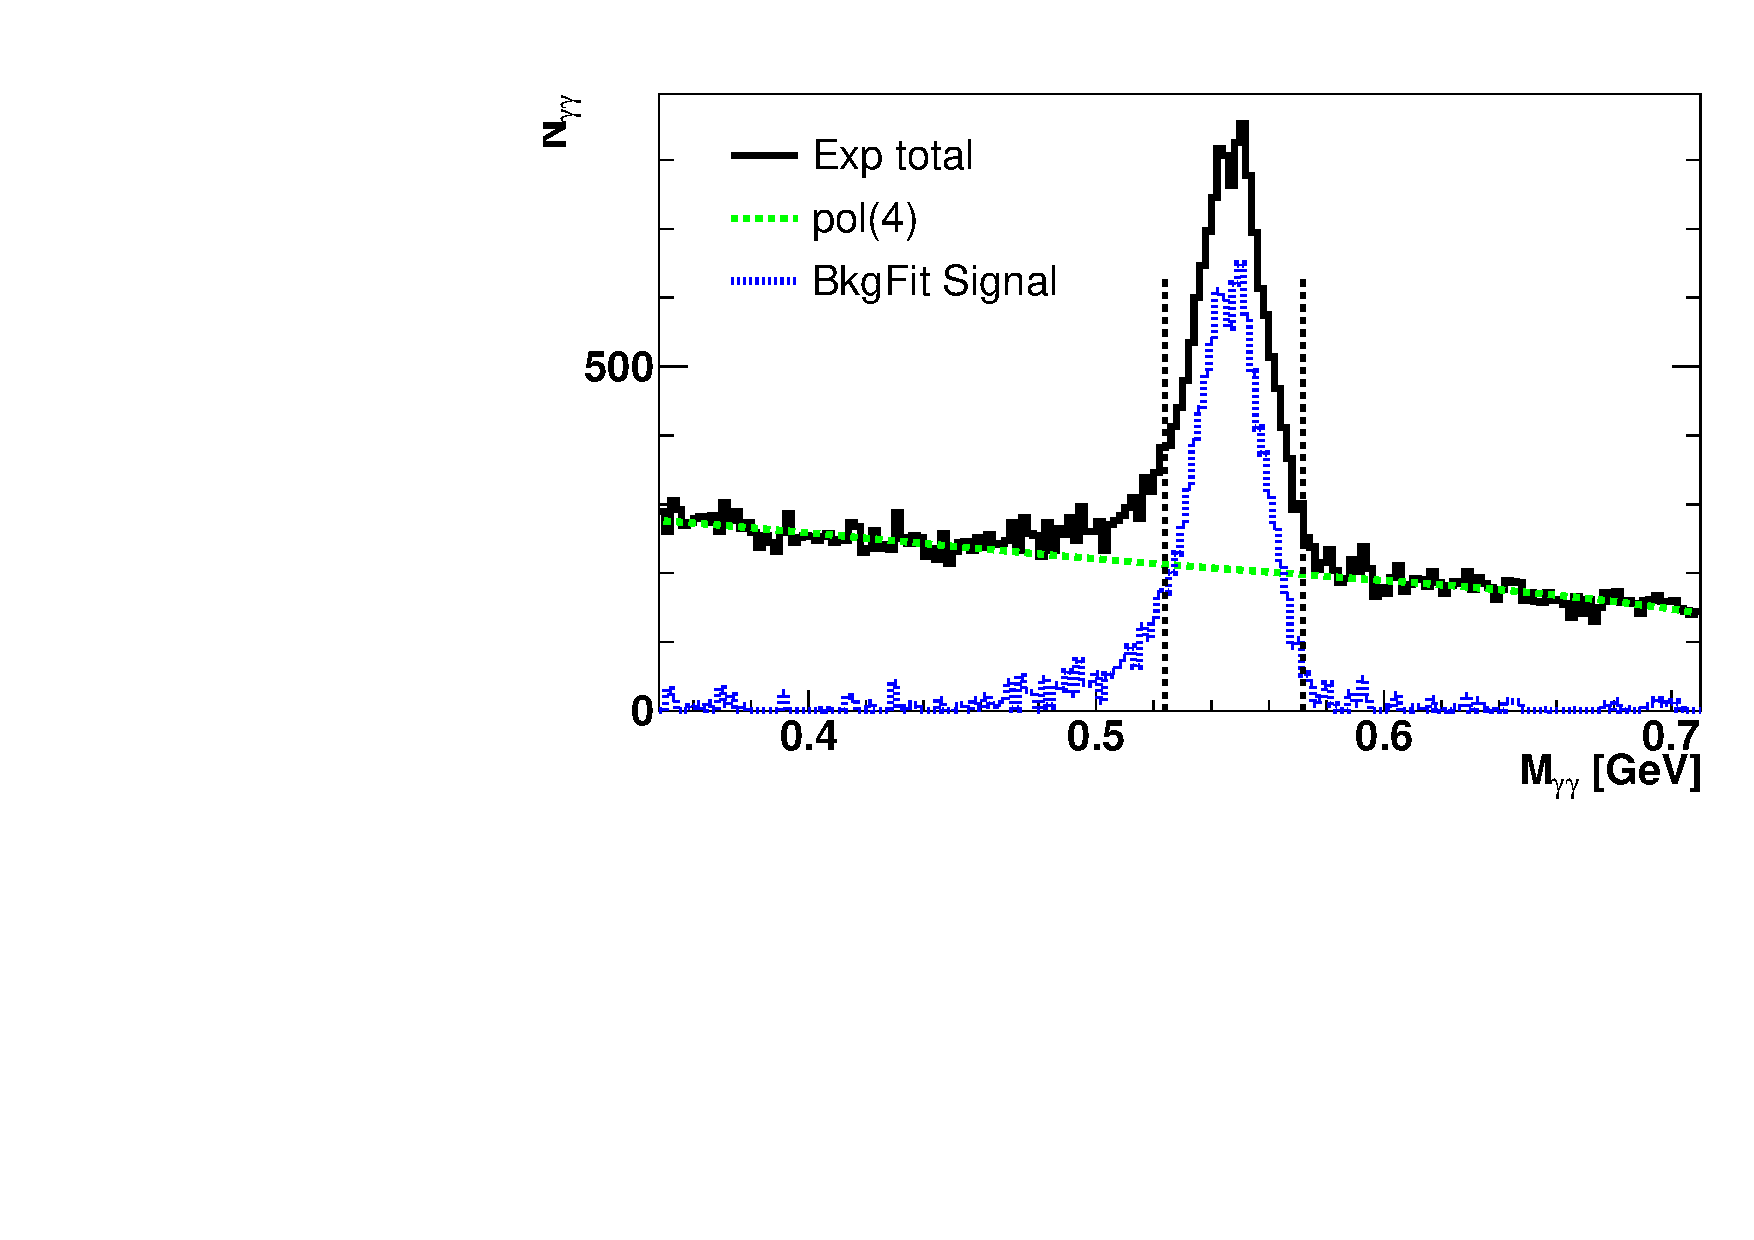
\includegraphics[width=.48\textwidth,natwidth=600,natheight=400]{figure_dataselection/eta_fitbkg_Z_4.pdf}}
\label{fig:etazfit}
\caption[Invariant-mass fits for $\eta$ in various \(z\) bins]{Invariant-mass fits for $\eta$ in various \(z\) bins (as labelled) as described in Section~\ref{sec:etafitsection}. Left (default fit):  a Crystal Ball for signal (red dashed line) and fifth-order polynomial for the background (green dotted line) are fit to data (black dash-dotted line), which is compared to the total fit  (cyan dash-dotted line). Right: only background is fitted using a fourth-order polynomial (green dotted line), while the signal (blue dotted line) is obtained by subtracting the background fit from data (black line).}
\end{figure}
\begin{figure}[H]  
 \centering 
 \subfigure[$z$ bin 5 ($0.6<z<0.7$)]{\label{fig:etafitz5}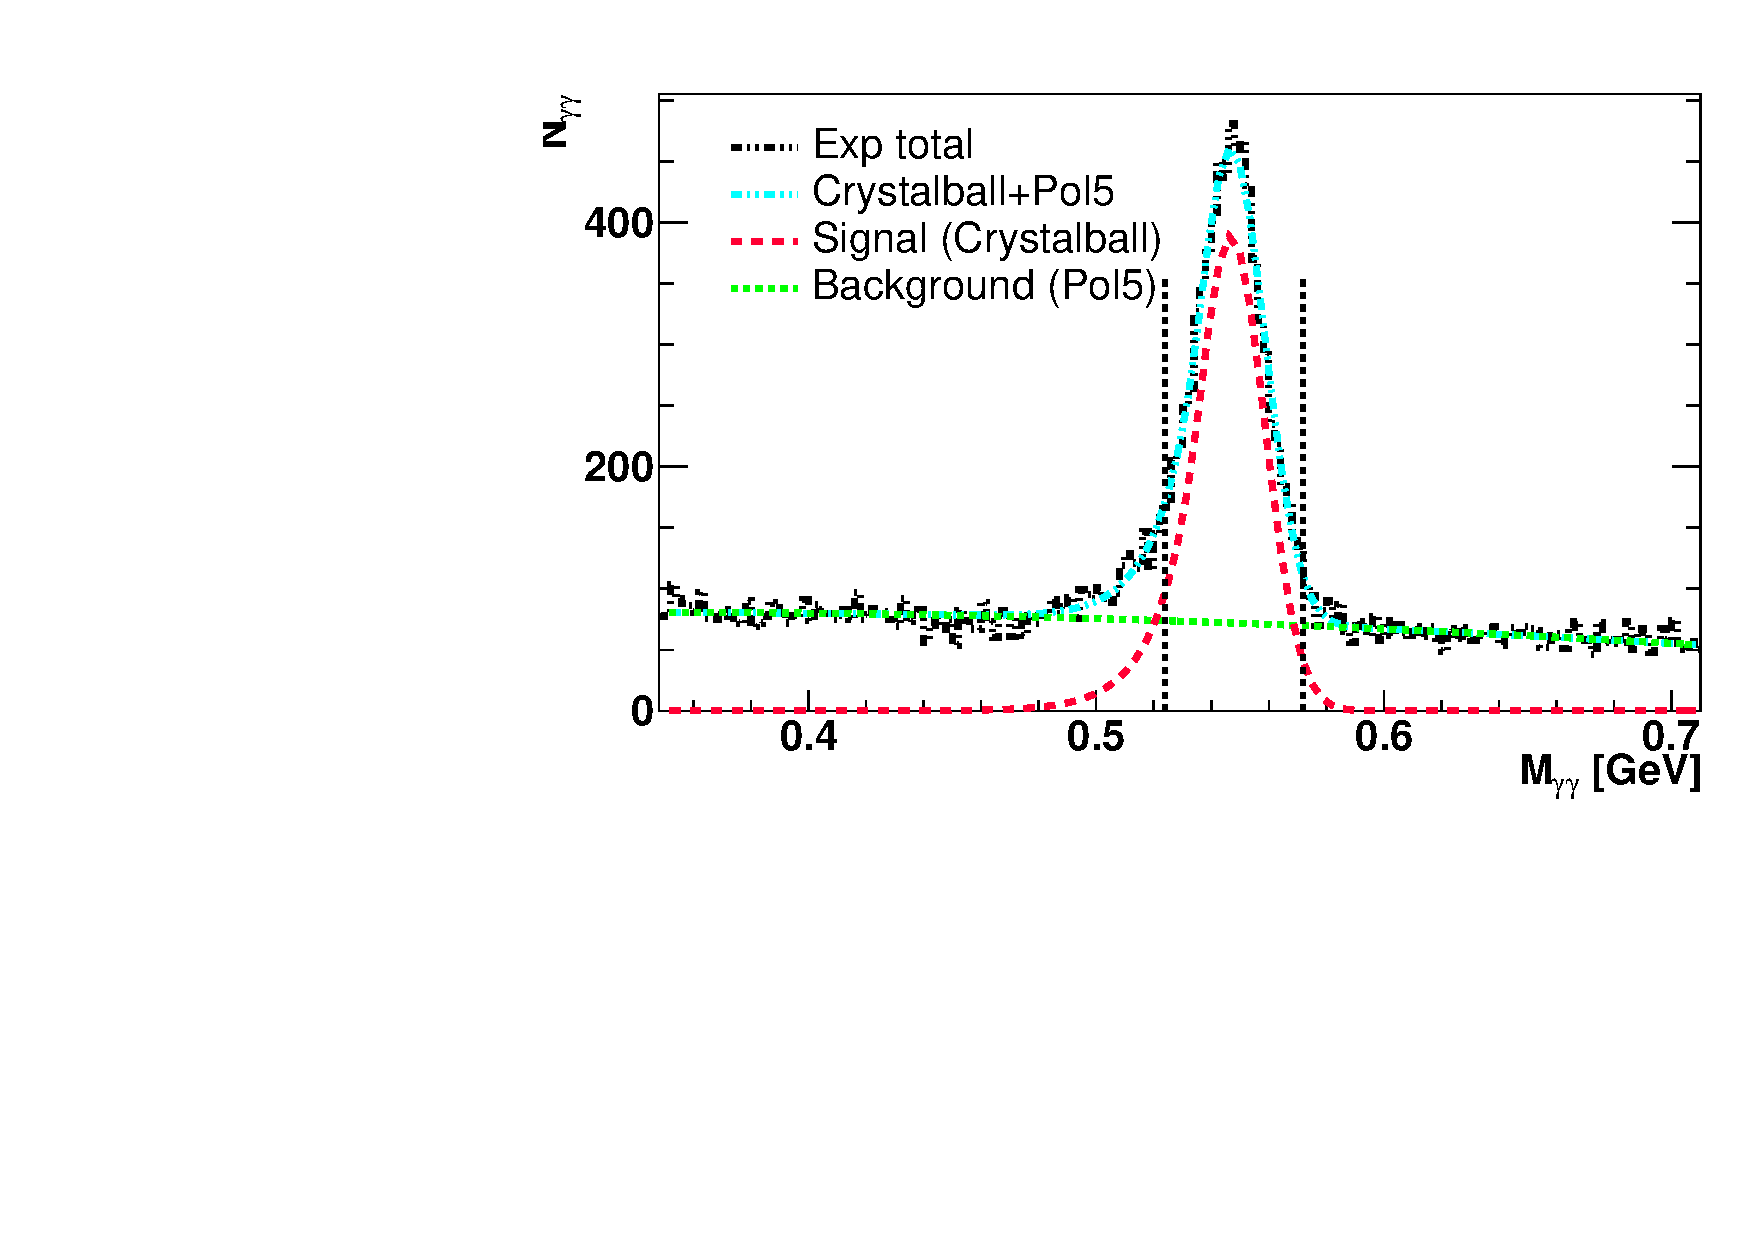
\includegraphics[width=.48\textwidth,natwidth=600,natheight=400]{figure_dataselection/eta_fitall_Z_5.pdf}}
 \subfigure[$z$ bin 5 ($0.6<z<0.7$)]{\label{fig:etafitz52}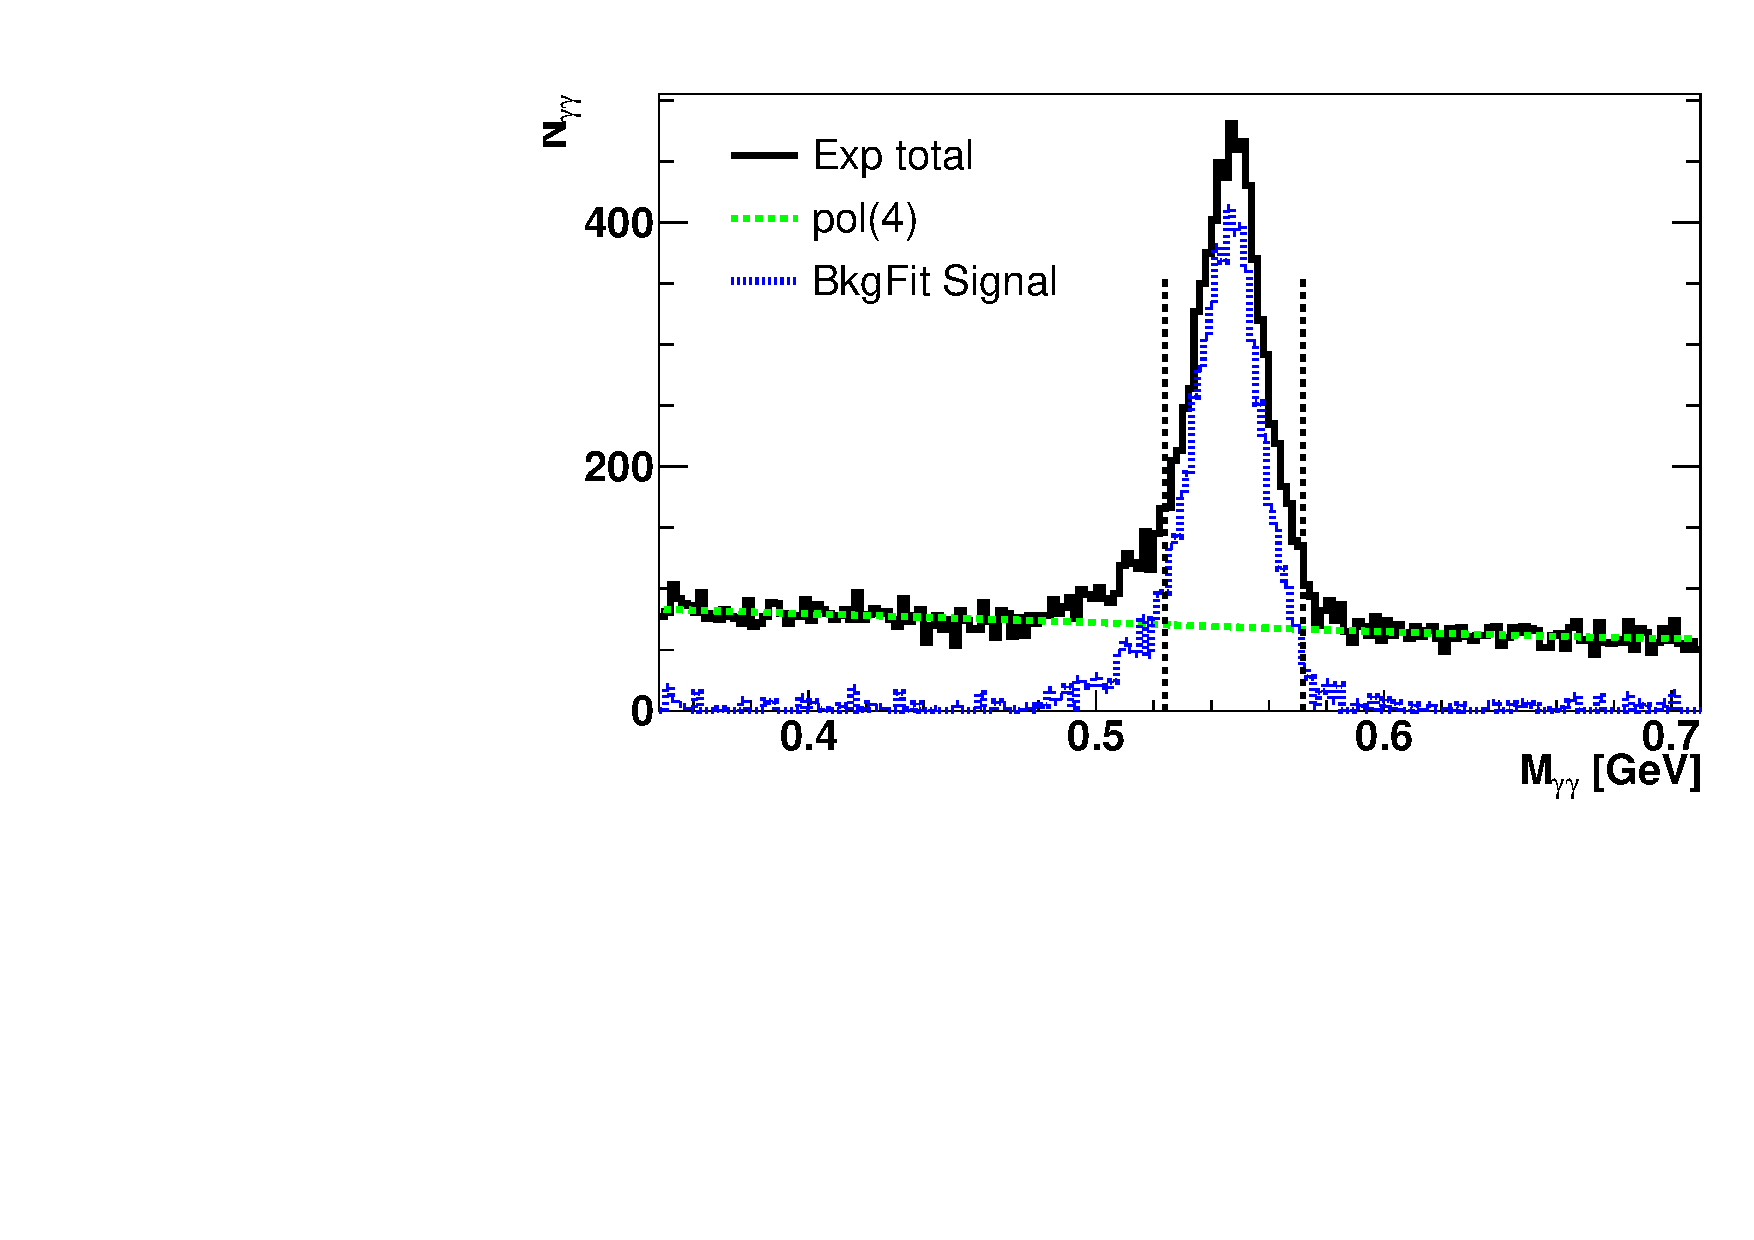
\includegraphics[width=.48\textwidth,natwidth=600,natheight=400]{figure_dataselection/eta_fitbkg_Z_5.pdf}}
 \subfigure[$z$ bin 6 ($0.7<z<1.0$)]{\label{fig:etafitz6}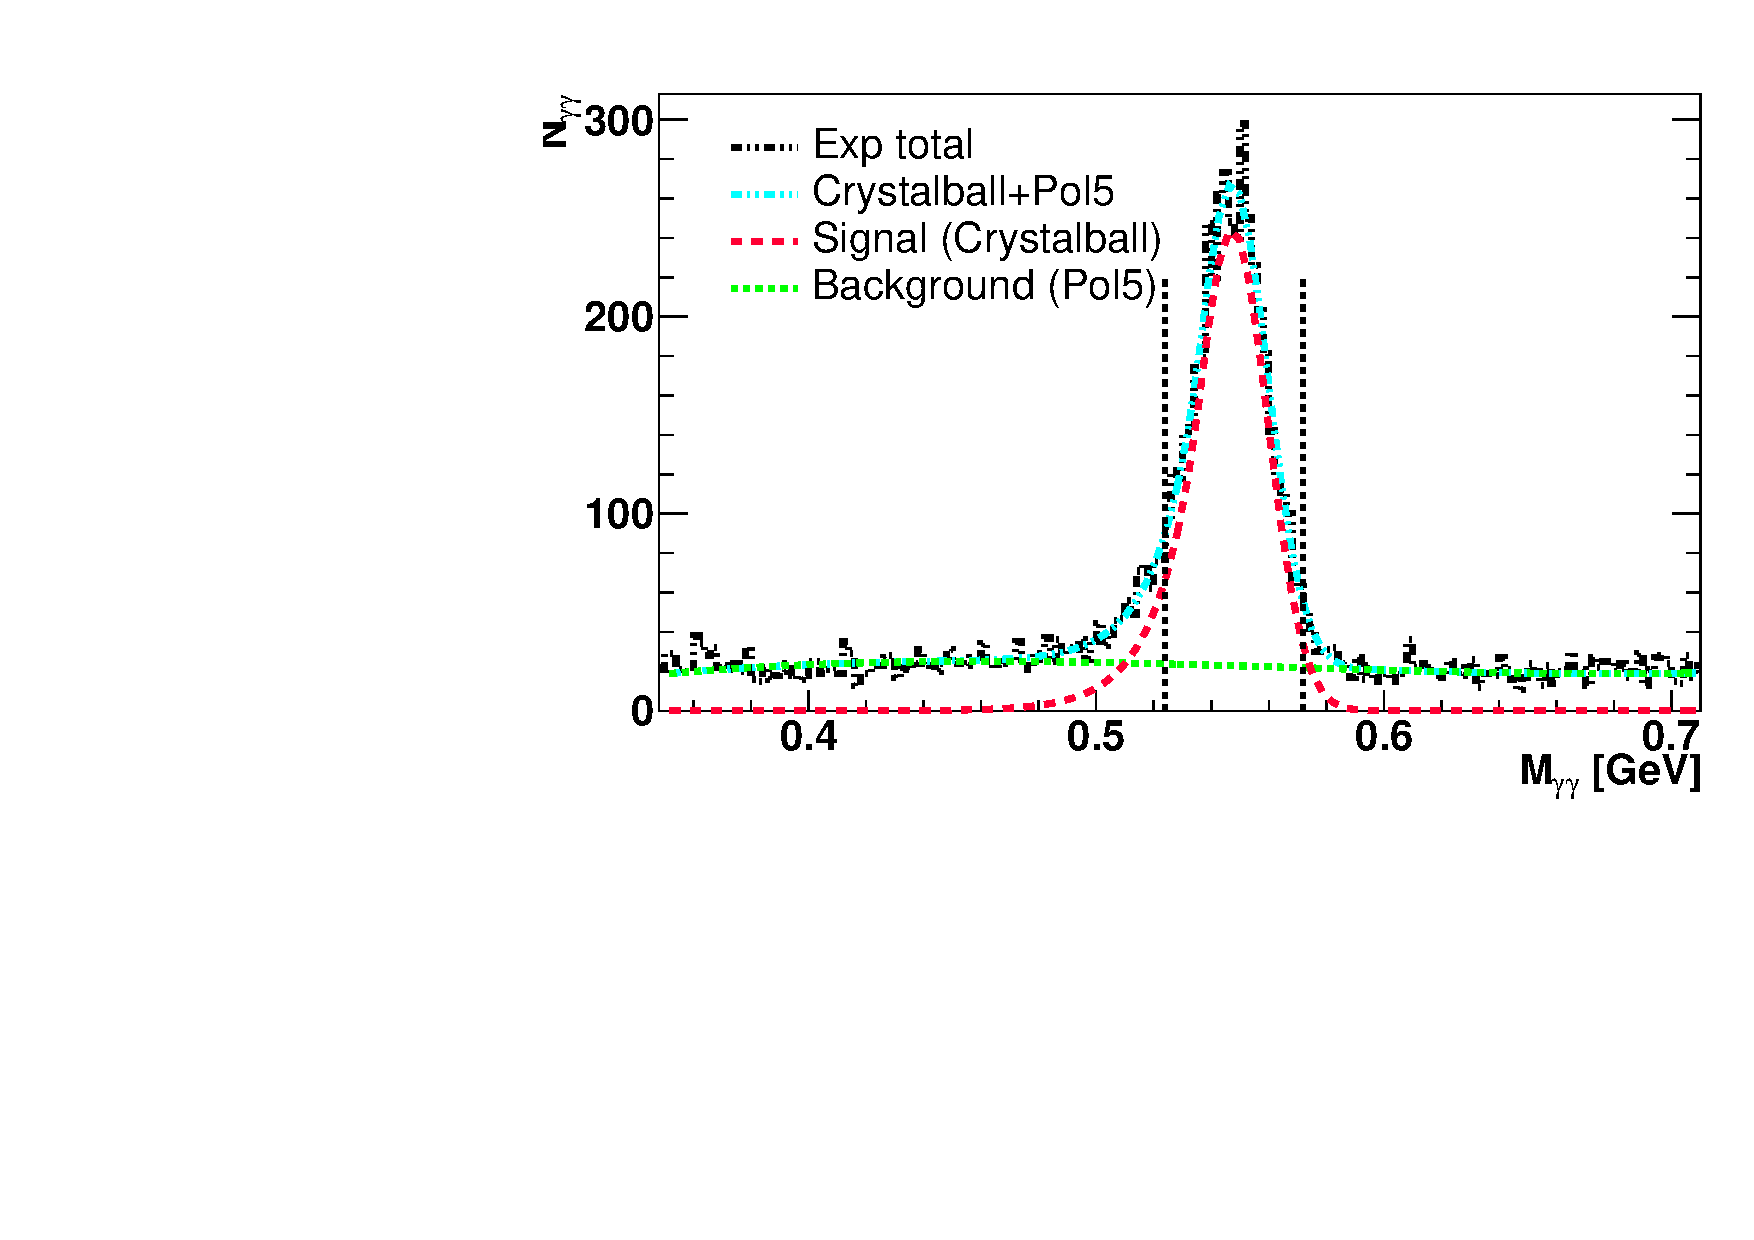
\includegraphics[width=.48\textwidth,natwidth=600,natheight=400]{figure_dataselection/eta_fitall_Z_6.pdf}}
 \subfigure[$z$ bin 6 ($0.7<z<1.0$)]{\label{fig:etafitz62}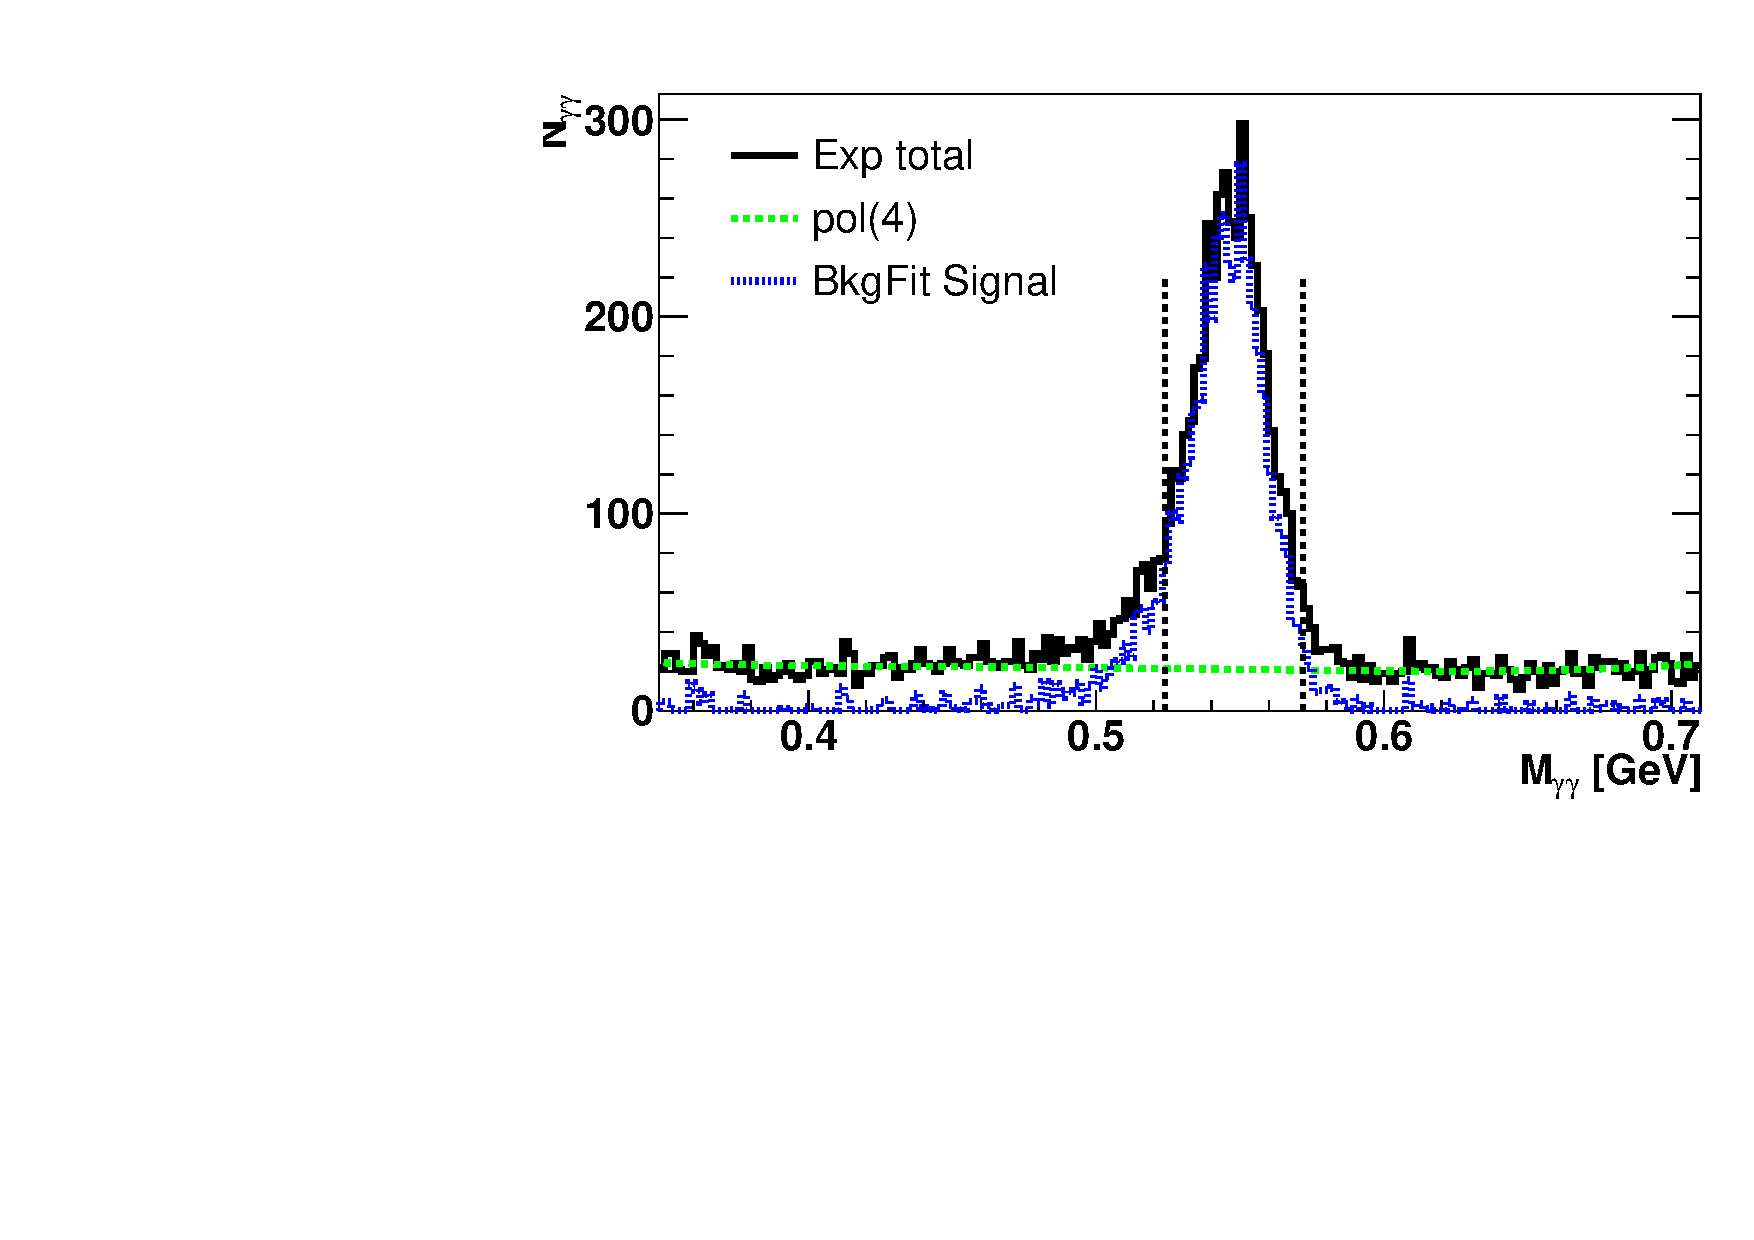
\includegraphics[width=.48\textwidth,natwidth=600,natheight=400]{figure_dataselection/eta_fitbkg_Z_6.pdf}}
\label{fig:etazfit}
\caption[Invariant-mass fits for $\eta$ in various \(z\) bins (cont.)]{(cont.) Invariant-mass fits for $\eta$ in various \(z\) bins (as labelled) as described in Section~\ref{sec:etafitsection}. Left (default fit):  a Crystal Ball for signal (red dashed line) and fifth-order polynomial for the background (green dotted line) are fit to data (black dash-dotted line), which is compared to the total fit  (cyan dash-dotted line). Right: only background is fitted using a fourth-order polynomial (green dotted line), while the signal (blue dotted line) is obtained by subtracting the background fit from data (black line).}
\end{figure}

\begin{figure}[H]
\ContinuedFloat*
 \centering
 \subfigure[$P_t$ bin 0 ($P_t<$ 0.15 GeV)]{\label{fig:etafitpt0}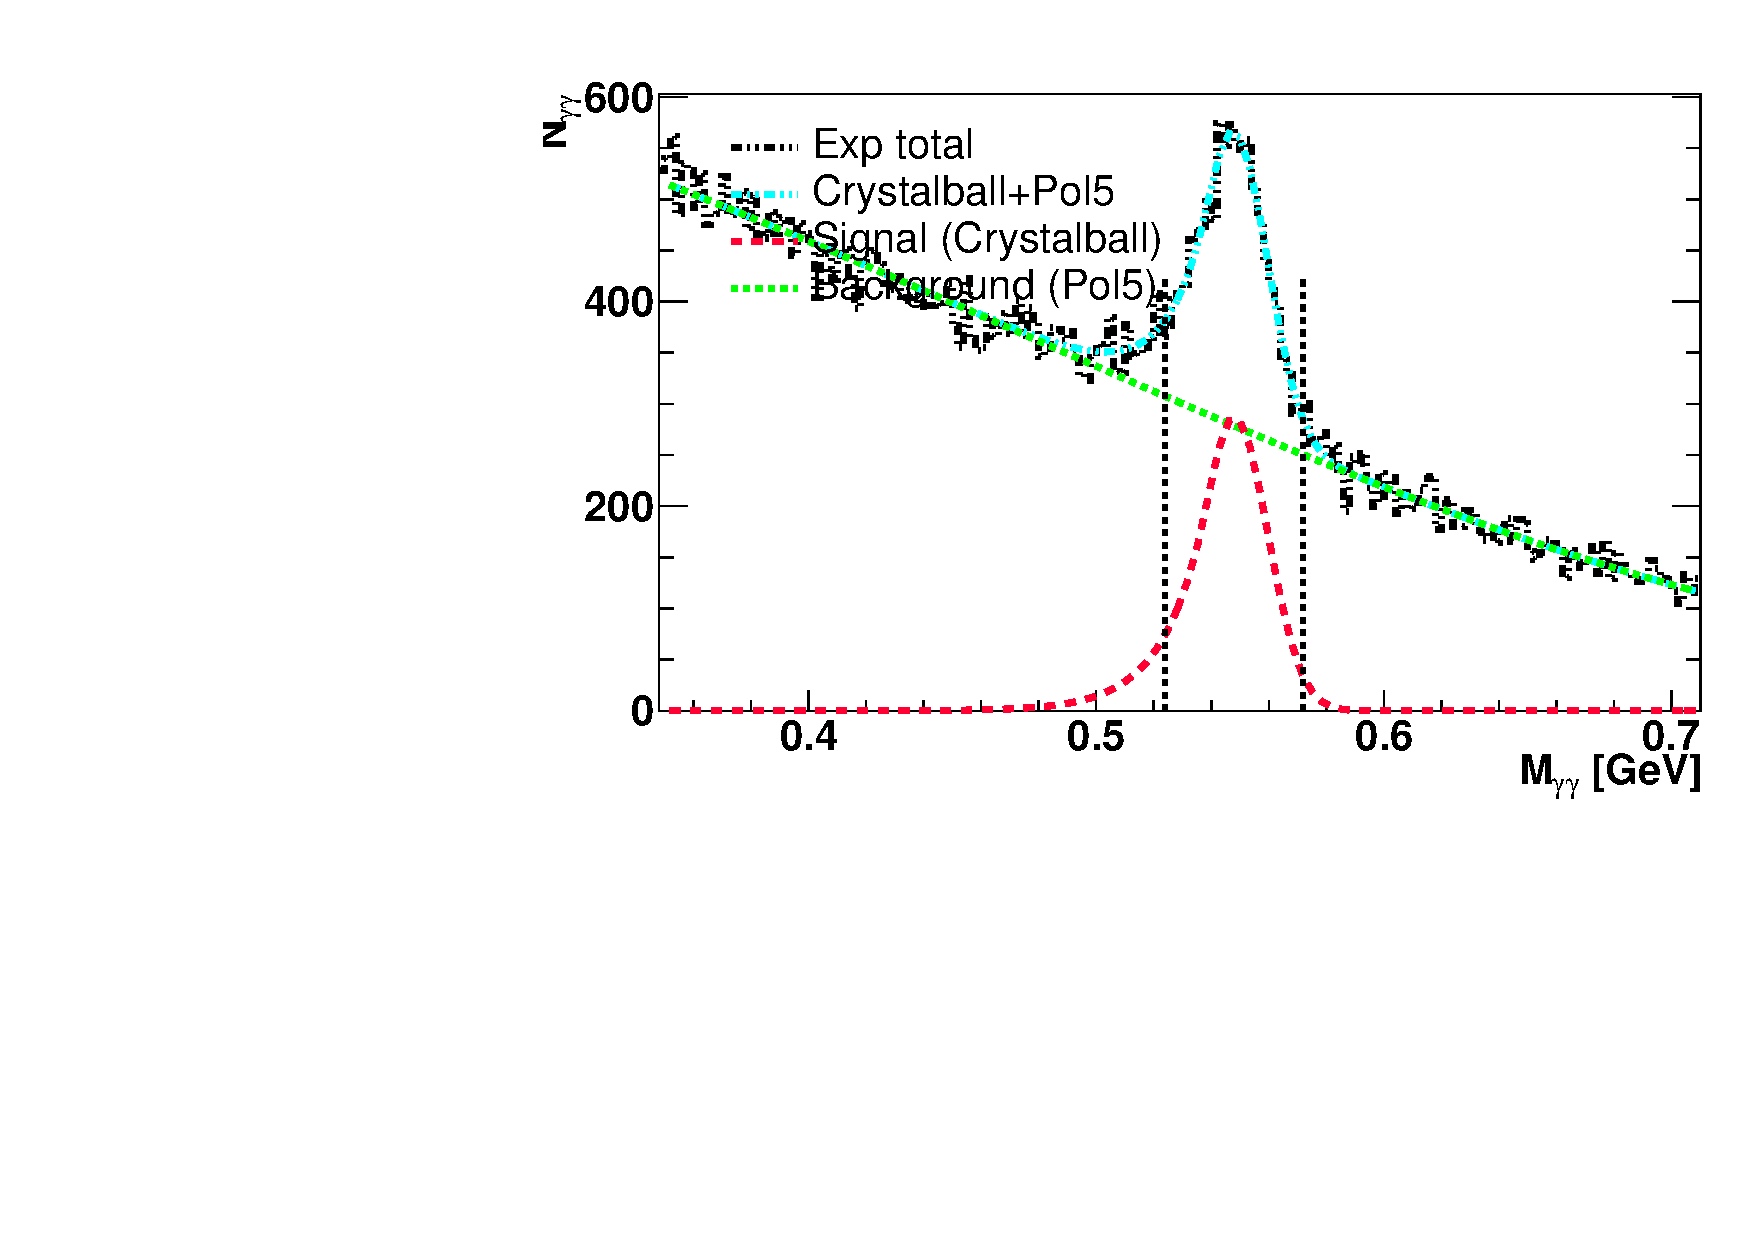
\includegraphics[width=.48\textwidth,natwidth=600,natheight=400]{figure_dataselection/eta_fitall_Pt_0.pdf}}
 \subfigure[$P_t$ bin 0 ($P_t<$ 0.15 GeV)]{\label{fig:etafitpt02}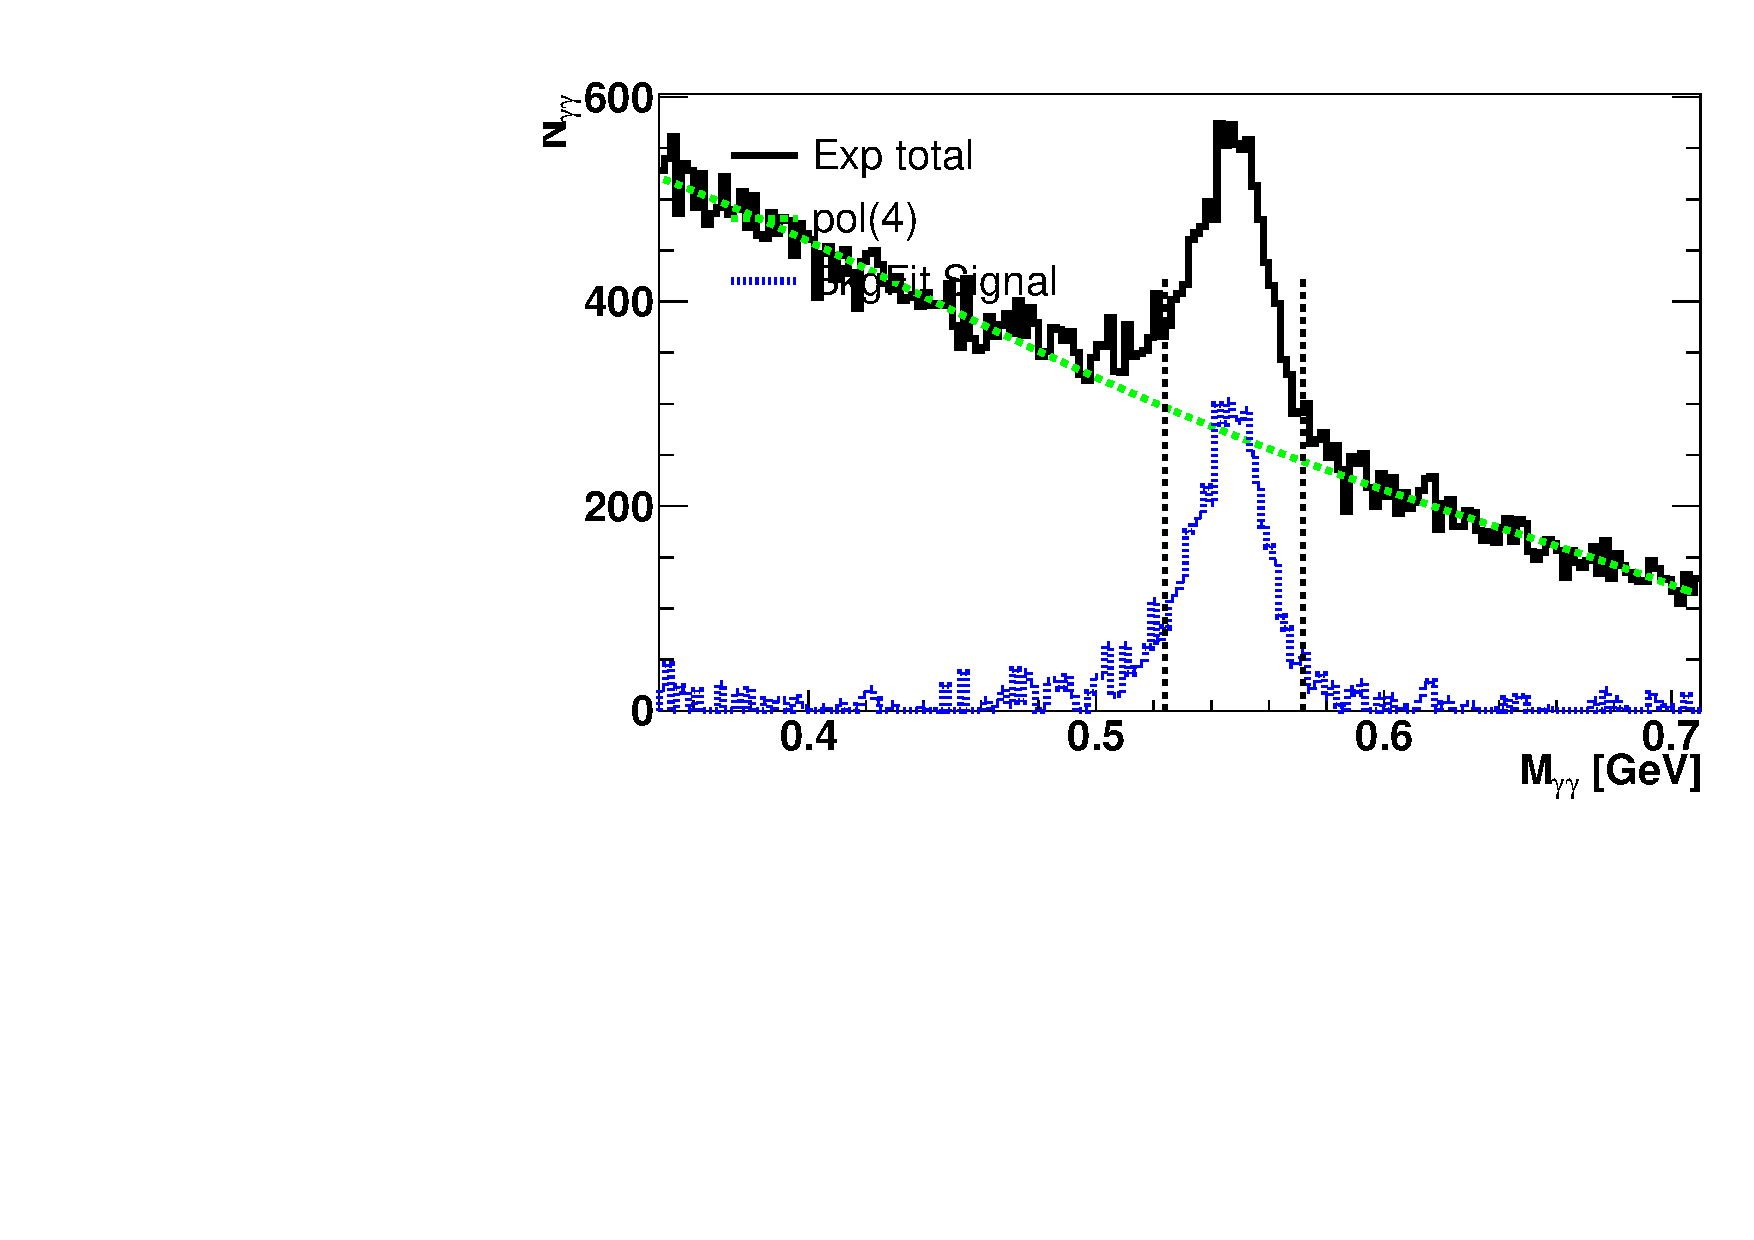
\includegraphics[width=.48\textwidth,natwidth=600,natheight=400]{figure_dataselection/eta_fitbkg_Pt_0.pdf}}
\label{fig:etaptfit}
\caption[Invariant-mass fits for $\eta$ in various \(P_{t}\) bins]{Invariant-mass fits for $\eta$ in various \(P_{t}\) bins (as labelled) as described in Section~\ref{sec:etafitsection}. Left (default fit):  a Crystal Ball for signal (red dashed line) and fifth-order polynomial for the background (green dotted line) are fit to data (black dash-dotted line), which is compared to the total fit  (cyan dash-dotted line). Right: only background is fitted using a fourth-order polynomial (green dotted line), while the signal (blue dotted line) is obtained by subtracting the background fit from data (black line).}
\end{figure}
\begin{figure}[H]   
 \centering 
 \subfigure[$P_t$ bin 1 (0.15 GeV $<P_t<$ 0.3 GeV)]{\label{fig:etafitpt1}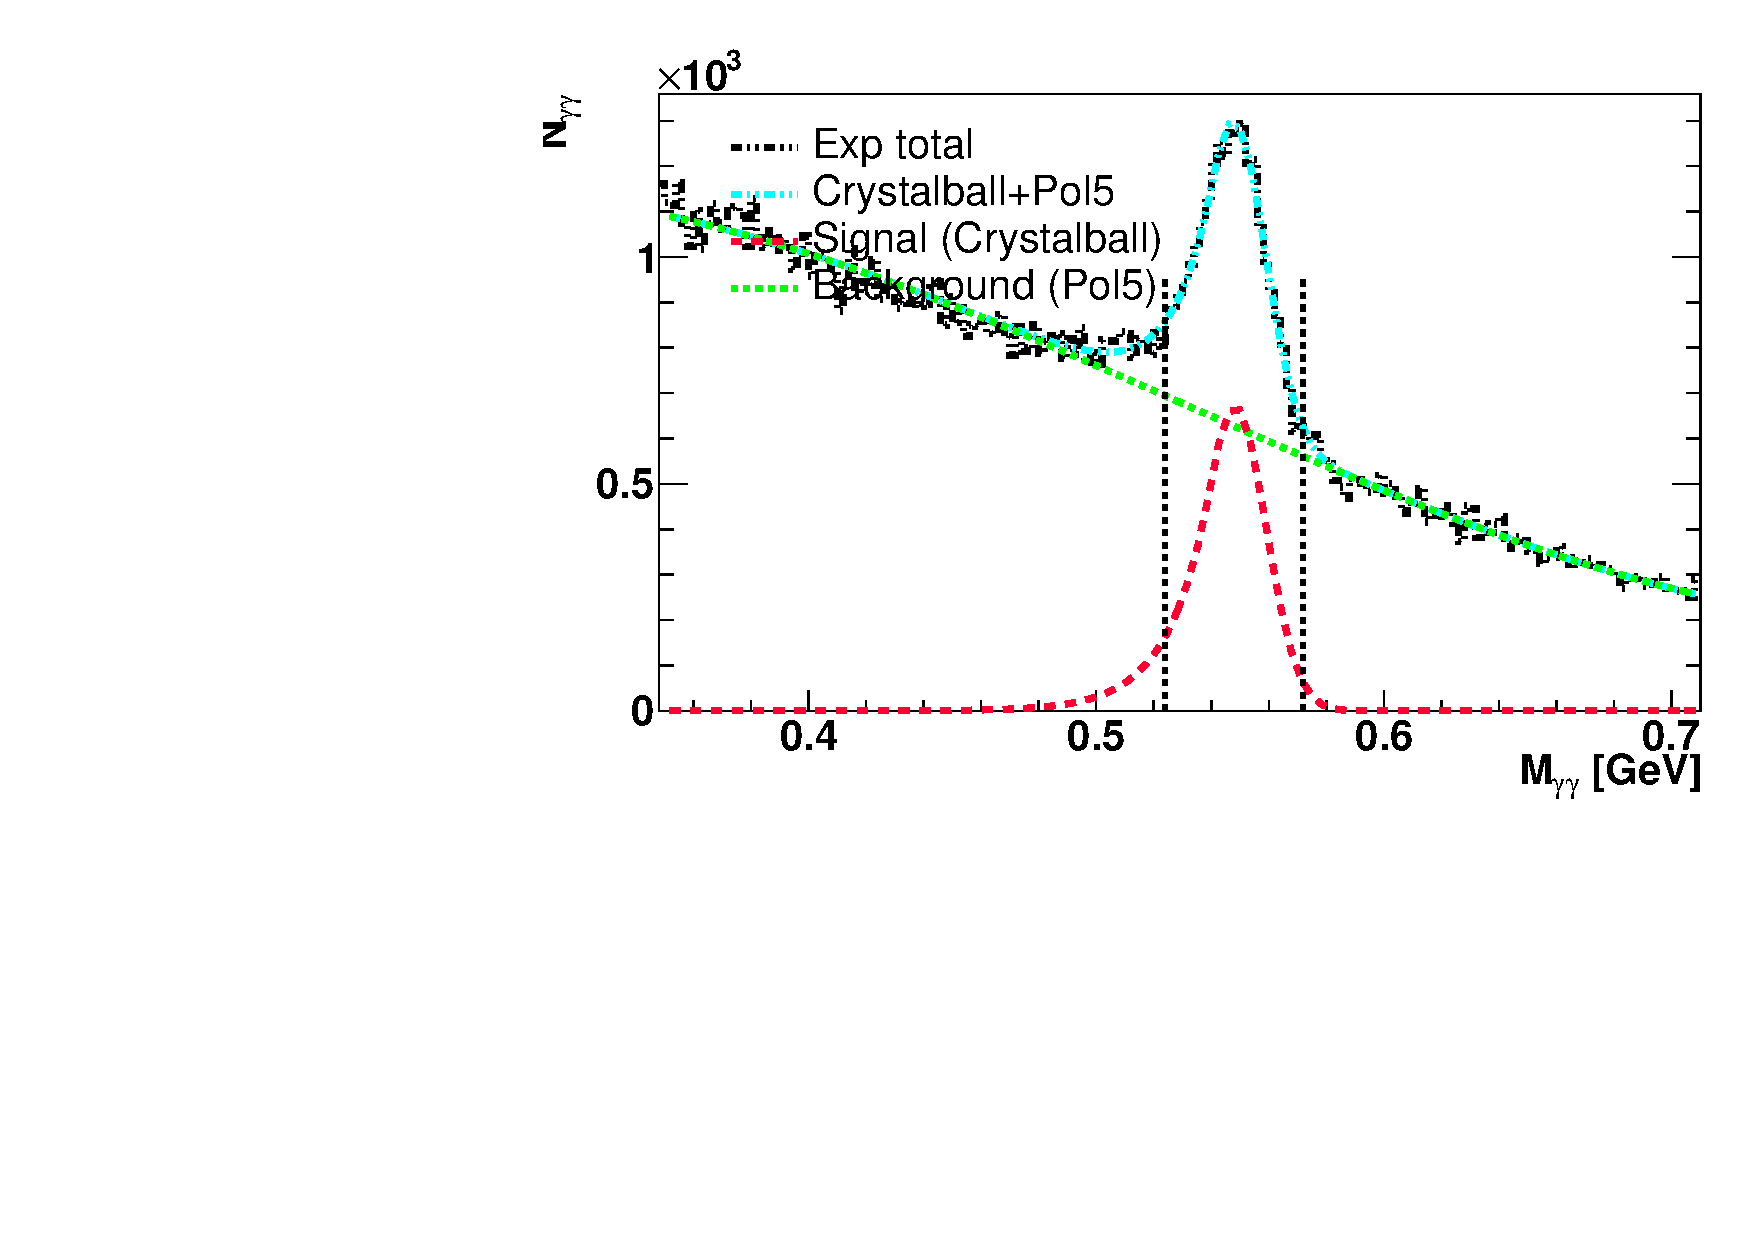
\includegraphics[width=.48\textwidth,natwidth=600,natheight=400]{figure_dataselection/eta_fitall_Pt_1.pdf}}
 \subfigure[$P_t$ bin 1 (0.15 GeV $<P_t<$ 0.3 GeV)]{\label{fig:etafitpt12}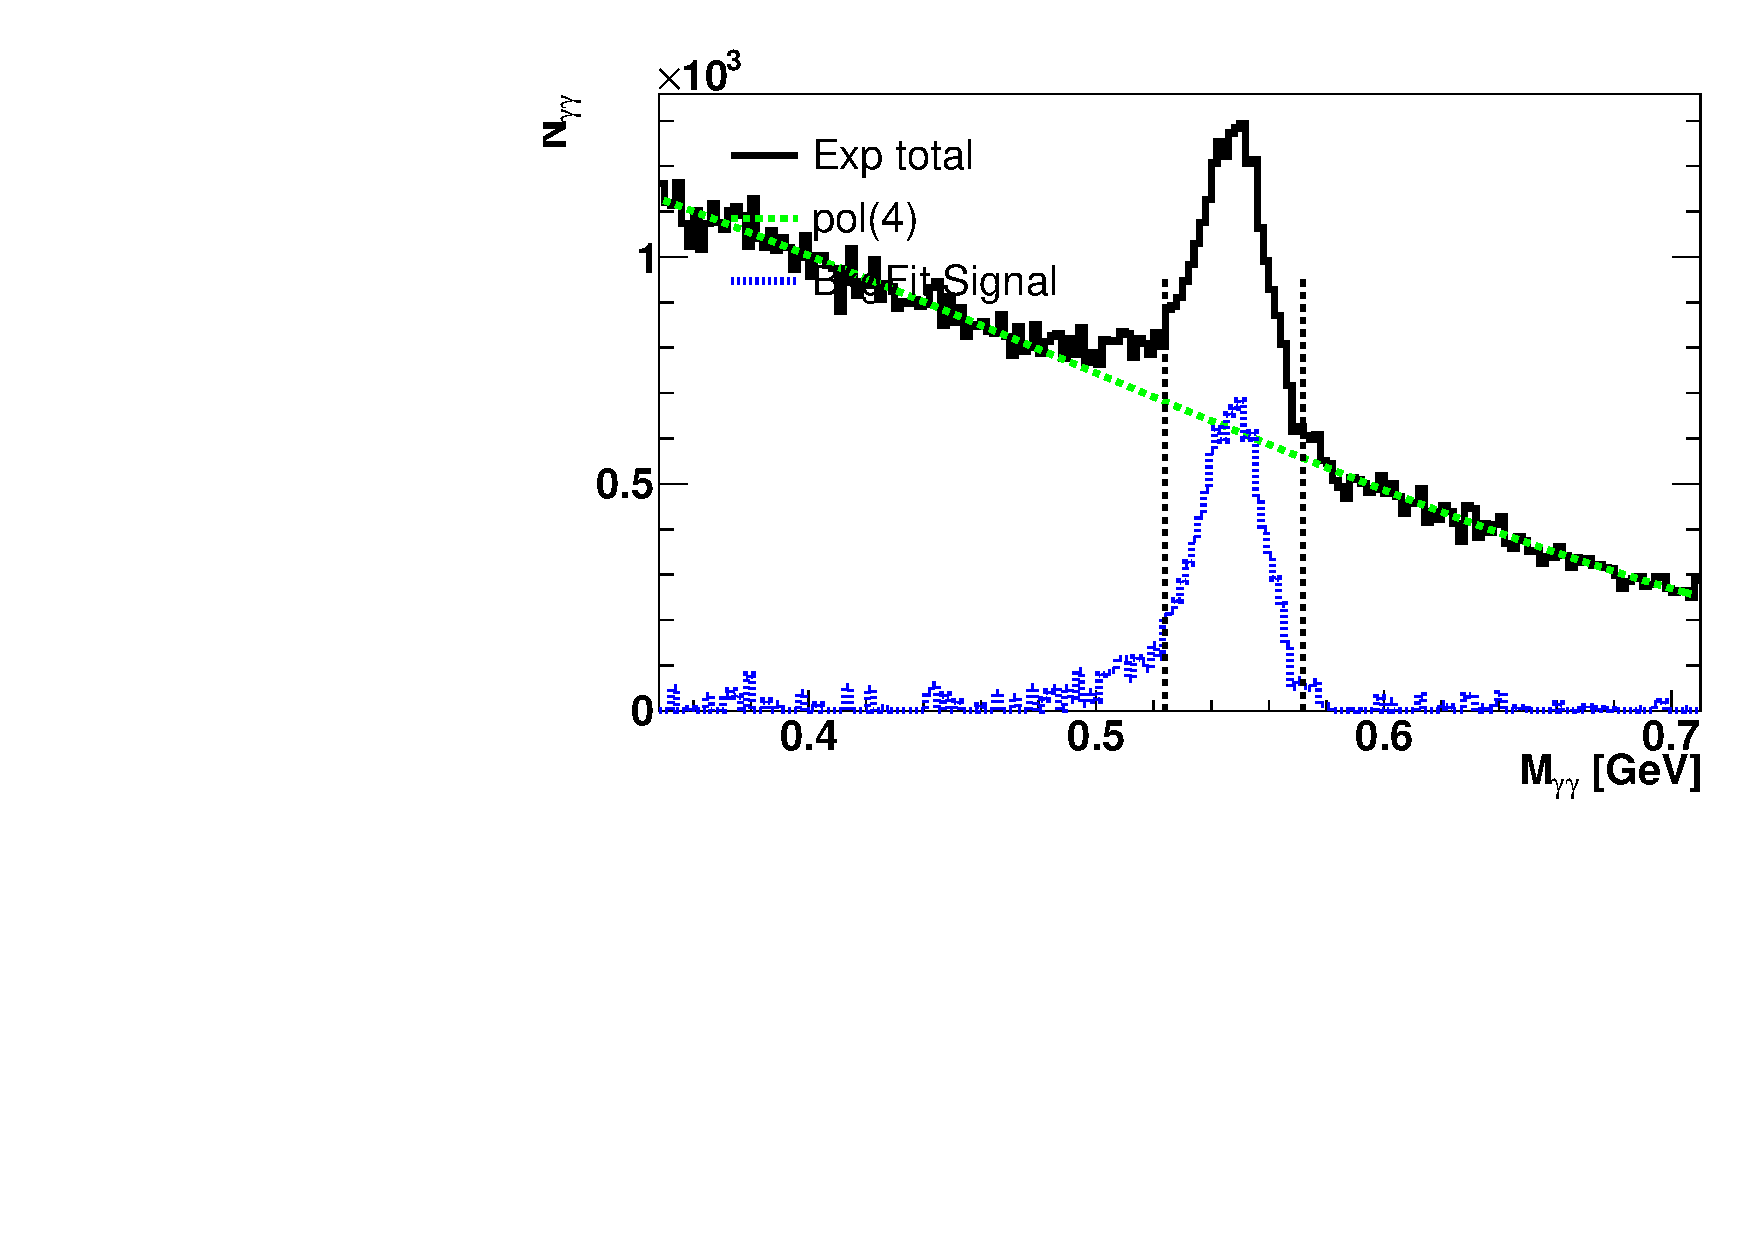
\includegraphics[width=.48\textwidth,natwidth=600,natheight=400]{figure_dataselection/eta_fitbkg_Pt_1.pdf}}
 \subfigure[$P_t$ bin 2 (0.3 GeV $<P_t<$ 0.5 GeV)]{\label{fig:etafitpt2}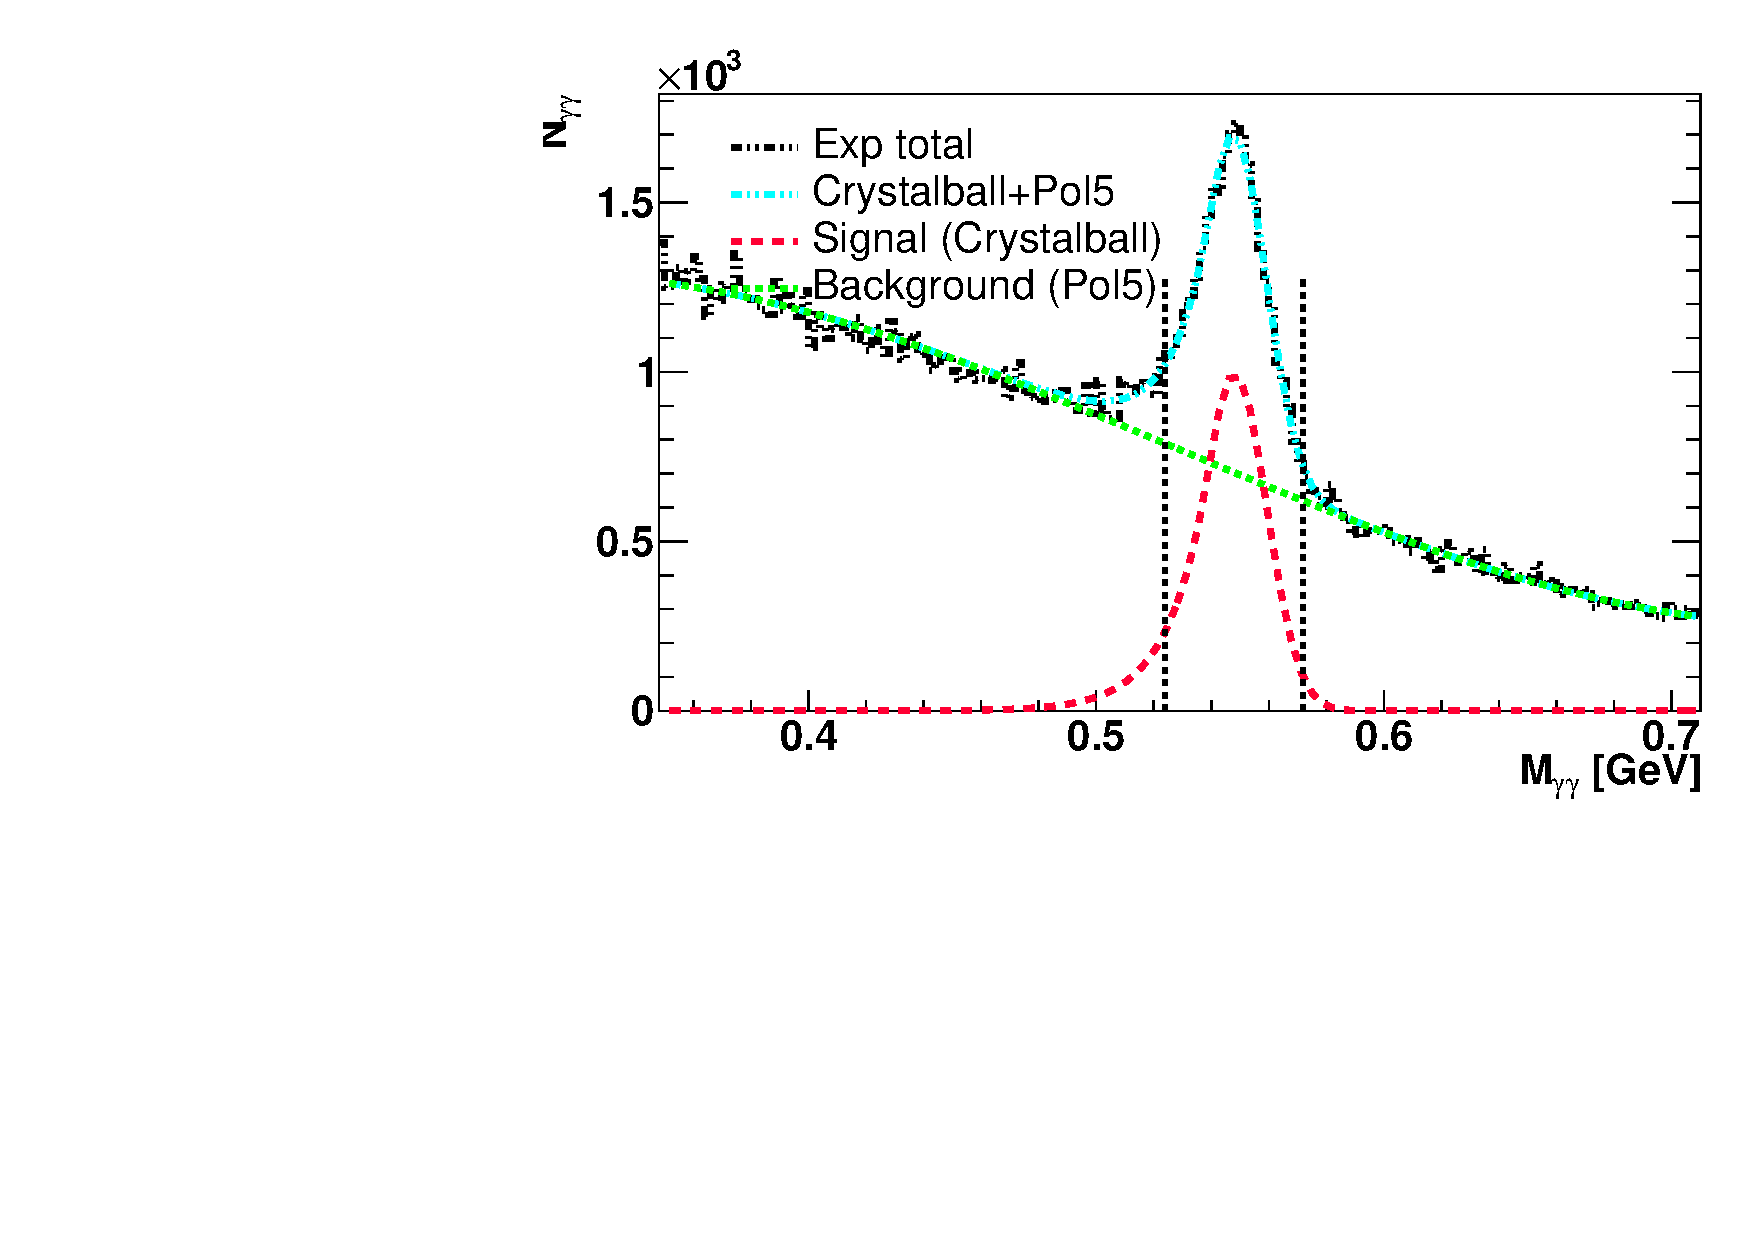
\includegraphics[width=.48\textwidth,natwidth=600,natheight=400]{figure_dataselection/eta_fitall_Pt_2.pdf}}
 \subfigure[$P_t$ bin 2 (0.3 GeV $<P_t<$ 0.5 GeV)]{\label{fig:etafitpt22}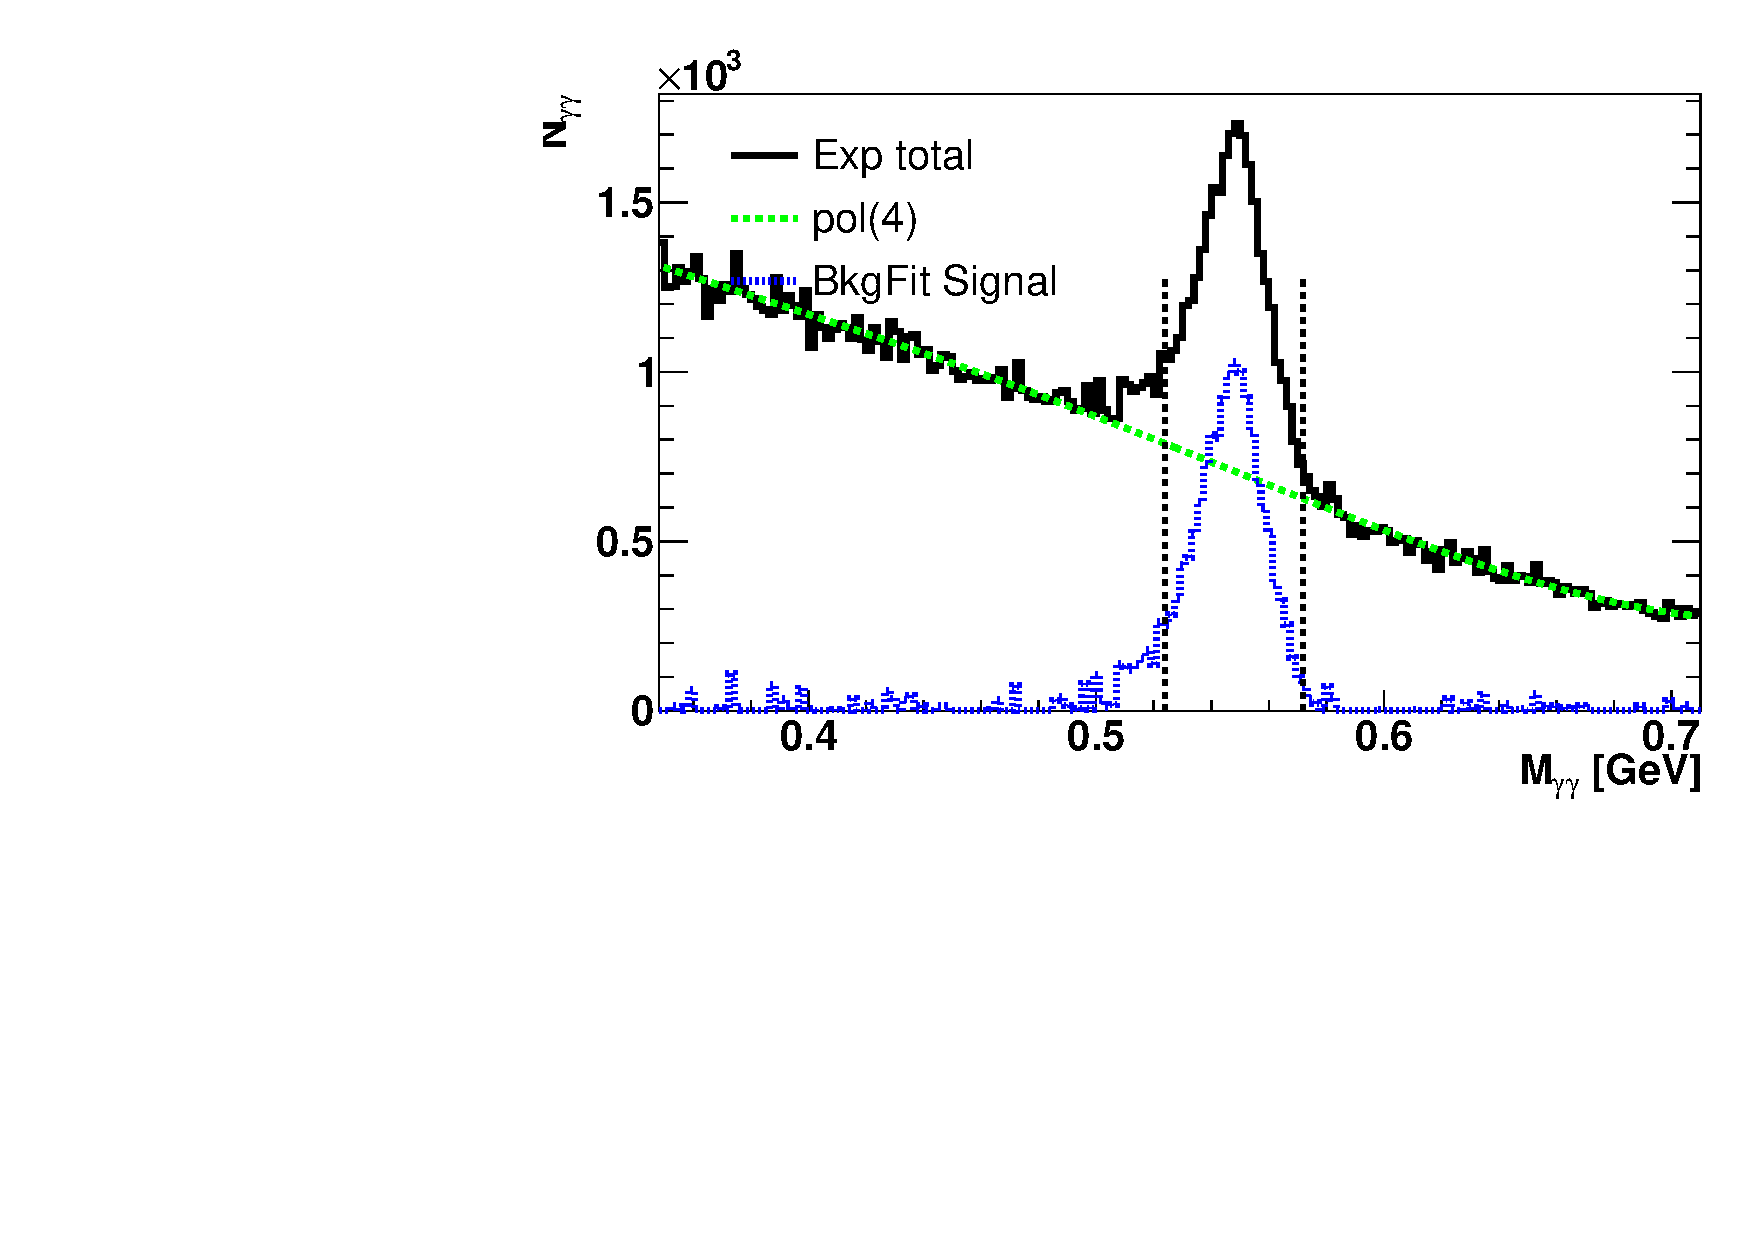
\includegraphics[width=.48\textwidth,natwidth=600,natheight=400]{figure_dataselection/eta_fitbkg_Pt_2.pdf}}
 \subfigure[$P_t$ bin 3 (0.5 GeV $<P_t<$ 3 GeV)]{\label{fig:etafitpt3}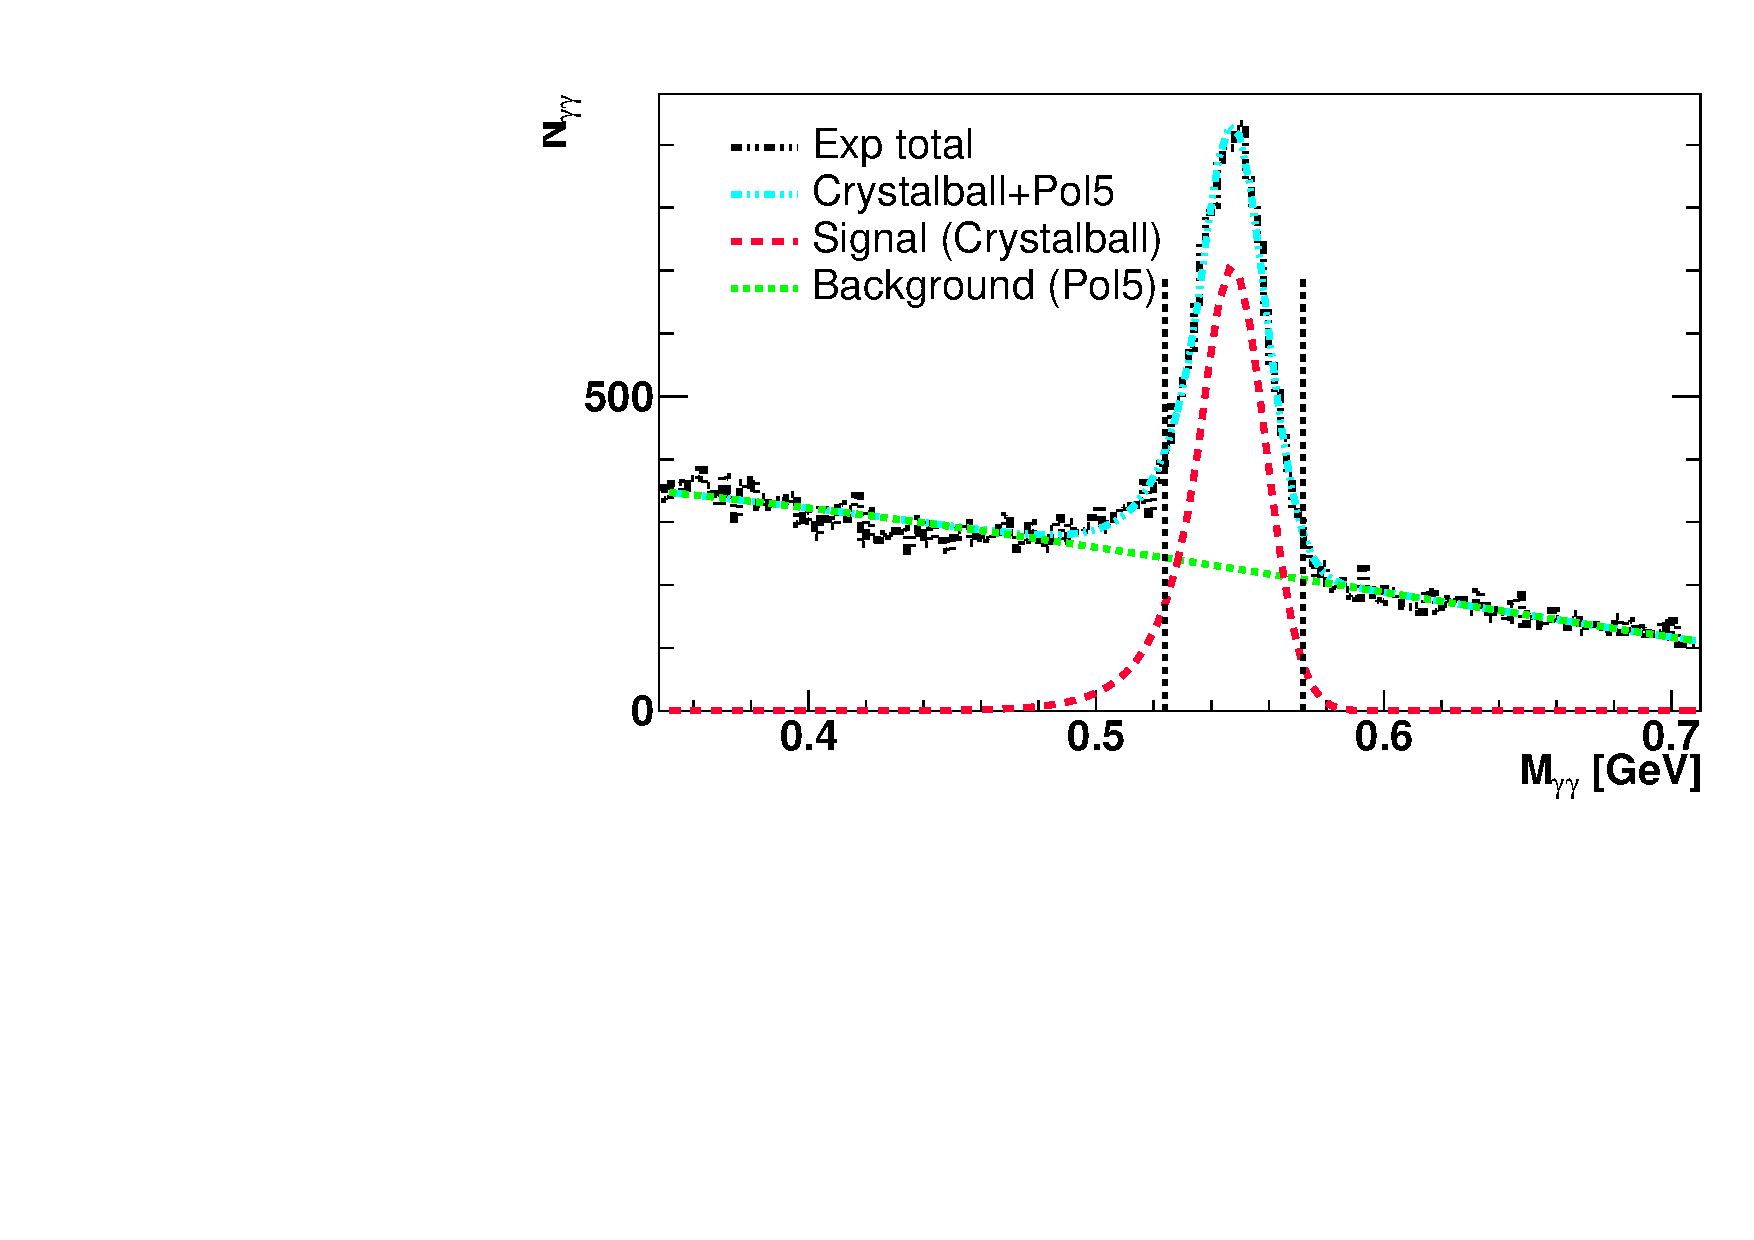
\includegraphics[width=.48\textwidth,natwidth=600,natheight=400]{figure_dataselection/eta_fitall_Pt_3.pdf}}
 \subfigure[$P_t$ bin 3 (0.5 GeV $<P_t<$ 3 GeV)]{\label{fig:etafitpt32}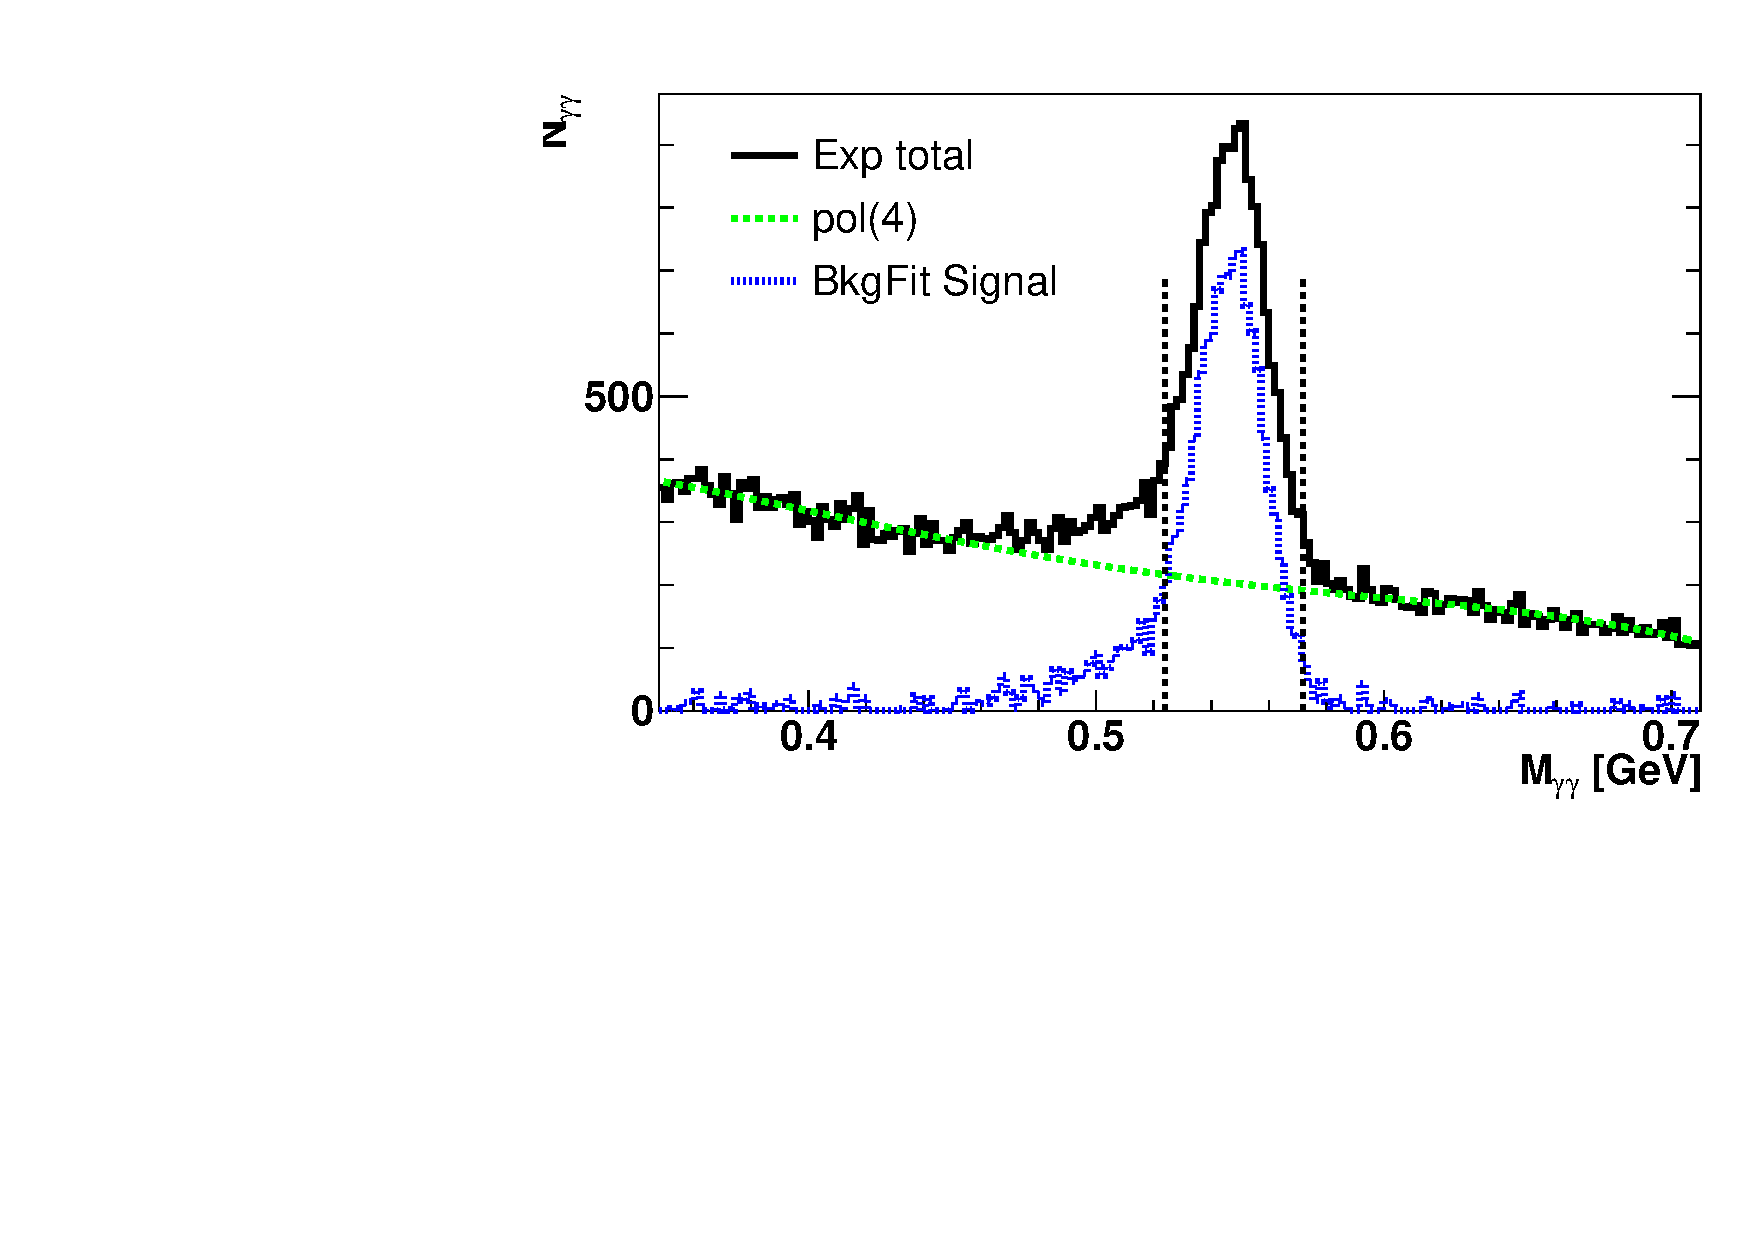
\includegraphics[width=.48\textwidth,natwidth=600,natheight=400]{figure_dataselection/eta_fitbkg_Pt_3.pdf}}
\caption[Invariant-mass fits for $\eta$ in various \(P_{t}\) bins (cont.)]{(cont.) Invariant-mass fits for $\eta$ in various \(P_{t}\) bins (as labelled) as described in Section~\ref{sec:etafitsection}. Left (default fit):  a Crystal Ball for signal (red dashed line) and fifth-order polynomial for the background (green dotted line) are fit to data (black dash-dotted line), which is compared to the total fit  (cyan dash-dotted line). Right: only background is fitted using a fourth-order polynomial (green dotted line), while the signal (blue dotted line) is obtained by subtracting the background fit from data (black line).}
  \label{fig:etaptfit}
\end{figure}
